\documentclass{beamer}
\usepackage{caption}
\captionsetup[figure]{labelformat=empty}
\usepackage[utf8]{inputenc}
%Load useful packages
\usepackage{graphicx} % Allows including images
\usepackage{booktabs} % Allows the use of \toprule, \midrule and \bottomrule in tables
\usepackage{subcaption,color}
\usepackage[table]{xcolor}
\usepackage{multirow}
\usepackage[most]{tcolorbox}

\usepackage{fontawesome5}
\usepackage{subfiles}
\usepackage{url}
\usepackage{amssymb,stmaryrd}
\usepackage{multimedia,bm}
\usepackage{bibentry}
\usepackage{algorithm,verbatim}
\usepackage{tikz,tikz-3dplot}
\usetikzlibrary{positioning,arrows,automata,external,hobby,decorations.pathreplacing,shapes,tikzmark}
\usetikzlibrary{overlay-beamer-styles}
\usetikzlibrary{arrows.meta}
\usetikzlibrary{matrix,calc}
\setbeamertemplate{navigation symbols}{}
\newcommand\intset[1]{\llbracket #1 \rrbracket}
\def\Ft{\mathbb{F}_t}
\definecolor{myyel}{RGB}{230,180,30}

\newcommand{\mc}[1]{\mathcal{#1}}
\newcommand{\supp}[0]{\mathtt{supp}}
\newcommand{\mb}[1]{\mathbb{#1}}
\def\xh{\widehat{x}}
\def\yh{\widehat{y}}
\def\R{\mathbb{R}}
\DeclareMathOperator{\round}{round}
\DeclareMathOperator{\diag}{diag}
\DeclareMathOperator{\rank}{rank}
\DeclareMathOperator{\fl}{fl}
\def\norm#1{\|#1\|}
\def\abs#1{|#1|}
\definecolor{mygreen}{RGB}{30, 190, 80}
%\definecolor{mygreen}{RGB}{30, 125, 120}
\newcommand{\eh}{\epsilon^H_i}
\newcommand{\eg}{\epsilon^g_i}
\newcommand{\ei}{\epsilon_i}
\newcommand{\limacc}{\gamma_i}
\def\hh{\widehat{h}}
\def\eps{\varepsilon}
\def\norminf#1{\|#1\|_\infty}


\graphicspath{{../POPILS/}{../Multilevel/}{../POPILS/images/}{../MPINNs_sorbonne/}{../../teaching/coursM2/figures/}{../../teaching/coursM2/MG/}{../../sparse_days/}{../slidesgiuseppe/}{../../../Documents/mixedai/presentations/PEQUAN_Apr2025_mixedDNN/}}

\newcommand{\smallRe}{\hbox{\footnotesize I\hskip -2pt R}}
\newcommand{\calA}{{\cal A}} 
\newcommand{\calB}{{\cal B}} 
\newcommand{\calD}{{\cal D}} 
\newcommand{\calF}{{\cal F}} 
\newcommand{\tim}[1]{\;\; \text{#1} \;\;}
\newcommand{\ms}{\;\;\;\;}
\newcommand{\opA}{{\mathrm{A}}}
\newcommand{\opD}{\mathrm{L}}
\newcommand{\D}{\mathrm{L}}
\usepackage{leftidx}
\newcommand{\Raw}{\rightarrow}
\usepackage{appendixnumberbeamer}
\definecolor{myblue}{RGB}{0,76,153}


\newtcolorbox{papirobox}{
    enhanced,
    colback=yellow!8!white,
    colframe=brown!60!black,
    boxrule=0.8pt,
    rounded corners=4pt,
    arc=4pt,
    drop shadow,
    left=8pt,
    right=8pt,
    top=5pt,
    bottom=5pt,
    width=0.95\textwidth
}

%%%%% Guillaume
\newcommand{\prox}{\operatorname{prox}}
\newcommand{\RR}{\mathbb{R}}
\newcommand{\Lo}{L}

%%%%% ML
\newcommand{\fsl}{f^{S_k^\ell}}
\newcommand{\fine}{\phi}
%\newcommand{\coarse}{\phi^H}
\newcommand{\coarse}{\phi}
\newcommand{\gk}{g_k}

\usepackage{tikz}
\usetikzlibrary{shapes.arrows}
\tikzset{
    myarrow/.style={
        draw,
        fill=orange,
        single arrow,
        minimum height=3.5ex,
        single arrow head extend=1ex
    }
}
\newcommand{\arrowright}{%
\tikz [baseline=-0.5ex]{\node [myarrow,rotate=-45] {};}
}
\newcommand{\arrowleft}{%
\tikz [baseline=-0.5ex]{\node [myarrow,rotate=-135] {};}
}


%\usepackage{algorithm}
\usepackage{algpseudocode,graphicx}
\newcommand\Fontvi{\fontsize{9}{9}\selectfont}
\newcommand\Fontvii{\fontsize{7}{7}\selectfont}
\newcommand\Fontviii{\fontsize{5}{5}\selectfont}
%Information to be included in the title page:
\title{Multilevel Physics Informed Neural Networks (MPINNs)}
\author{\underline{Elisa Riccietti}\\[3mm]
%\vspace{1cm}
Joint work with: S. Gratton - V. Mercier (IRIT), P. Toint (UNamur)}
\institute{LIP - ENS Lyon}
%\author{Valentin Mercier, \underline{Elisa Riccietti}, Serge Gratton, Philippe Toint}
%\institute{IRIT / \underline{ENS Lyon} / UNamur}


\date{\today}
%Logo in every slide

%%setting up some useful slide creation commands
%split slide
\newenvironment{splitframe}[5]
%[1] ==> 1 parameter passed through {}
%[2] ==> 2 parameters passed through {}{}
%[4] ==> 4 parameters passed through {}{}{}{}
    {
    \begin{frame}{#3}
    \begin{columns}
    \column{#1\linewidth}
    \centering
    #4
    \column{#2\linewidth}
    \centering
    #5
    \end{columns}
    \centering
    \vspace{\baselineskip} % adds one line space
    }
    %Inside the first pair of braces (ABOVE) is set what your new environment will do before the text within, then inside the second pair of braces (BELOW) declare what your new environment will do after the text. Note second pair can be empty braces too.
    {
    \end{frame}
    }
\AtBeginSection[]
{
    \begin{frame}
        \frametitle{Outline}
        \tableofcontents[currentsection]
    \end{frame}
}

\makeatletter
\renewcommand{\ALG@beginalgorithmic}{\small}
\makeatother



\begin{document}
%\setbeamertemplate{footline}[page number]
\addtobeamertemplate{navigation symbols}{}{%
    \usebeamerfont{footline}%
    \usebeamercolor[fg]{footline}%
    \hspace{1em}%
    \insertframenumber/\inserttotalframenumber
}
\begin{frame}
  \begin{center}
    \textbf{\LARGE  \alert{Exploiting hierarchical structures
in numerical optimization}}
    \vspace{0.5cm}
      \end{center}
    \begin{columns}
    \begin{column}{0.6\textwidth}
    \textbf{ \alert{}}

    \vspace{0.5cm}
    \textbf{\underline{Elisa Riccietti} - LIP-ENS Lyon
    %and\\
   % Théo Mary
   }
   
   
    \vspace{0.5cm}
      \textbf{}
      
     \vspace{0.2cm}
      \textbf{}

     \vspace{1cm}
      HDR defence 28/09/2026      \includegraphics[scale=0.2]{../../loghi_firme/logo.png}
     \end{column}
    \begin{column}{0.4\textwidth}
  %  \includegraphics[width=0.8\textwidth]{images/grids.png}
     \centering
 \includegraphics[width=0.5\textwidth]{unc_sol.eps}    
 \includegraphics[width=0.5\textwidth]{sol_2.eps}    
\includegraphics[width=0.5\textwidth]{sol_1.eps}    


    \vfill
   

       \end{column}
            \end{columns}
             \end{frame}
  






  \begin{frame}{The context}
  
\begin{columns}[T,onlytextwidth]

\begin{column}{0.5\textwidth}
\begin{tcolorbox}[
 title={The problem},
    colback=red!10,
    colframe=red!70!black,
        fonttitle=\bfseries,
        ]
        
       $$\min_{x\in\R^{\alert{n}}} f(x)$$
              $f$ \alert{non-linear, non-convex}\\
        $n$ \alert{very large} 
      
       
       \vspace{0.65cm}
       \begin{tiny}
       {\bf Examples:}
       \begin{itemize}
       \item Image restoration
       \item Matrix factorization
       \item Neural networks training
       \end{itemize}
       \end{tiny}
\end{tcolorbox}
\end{column}

\begin{column}{0.48\textwidth}
\begin{tcolorbox}[
 title={A special class of pbs. },
    colback=green!10,
    colframe=green!70!black,
        fonttitle=\bfseries,
        ]
        
    \vspace{0.1cm}
     \centering   
  \alert{Hierarchically structured} problems
    
           
    \centering
   %   
\includegraphics[width=0.7\textwidth]{MG}\\
  \includegraphics[width=0.6\textwidth]{figures/grids.png}
   % 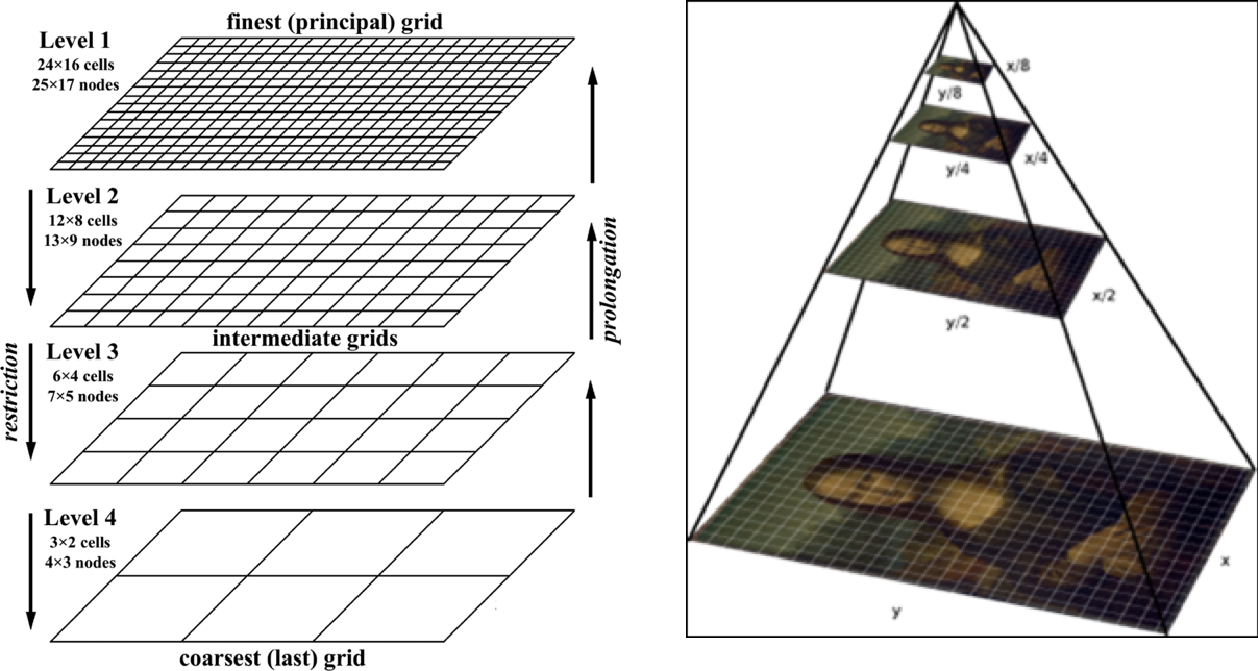
\includegraphics[width=\textwidth]{figures/structured}

   \vspace{-0.25cm}
  \phantom{a}
\end{tcolorbox}


\end{column}
\end{columns}
\begin{tcolorbox}[
 title={Objective},
    colback=orange!10,
    colframe=orange!70!black,
        fonttitle=\bfseries,
        ]
        
     Exploit hierarchical structures to develop \alert{parsimonious} and \alert{efficient} mathematically founded algorithms
     
     \end{tcolorbox}


\end{frame}


\begin{frame}{Outline: explore the notion of hierarchy in different contexts}



\begin{figure}
\centering
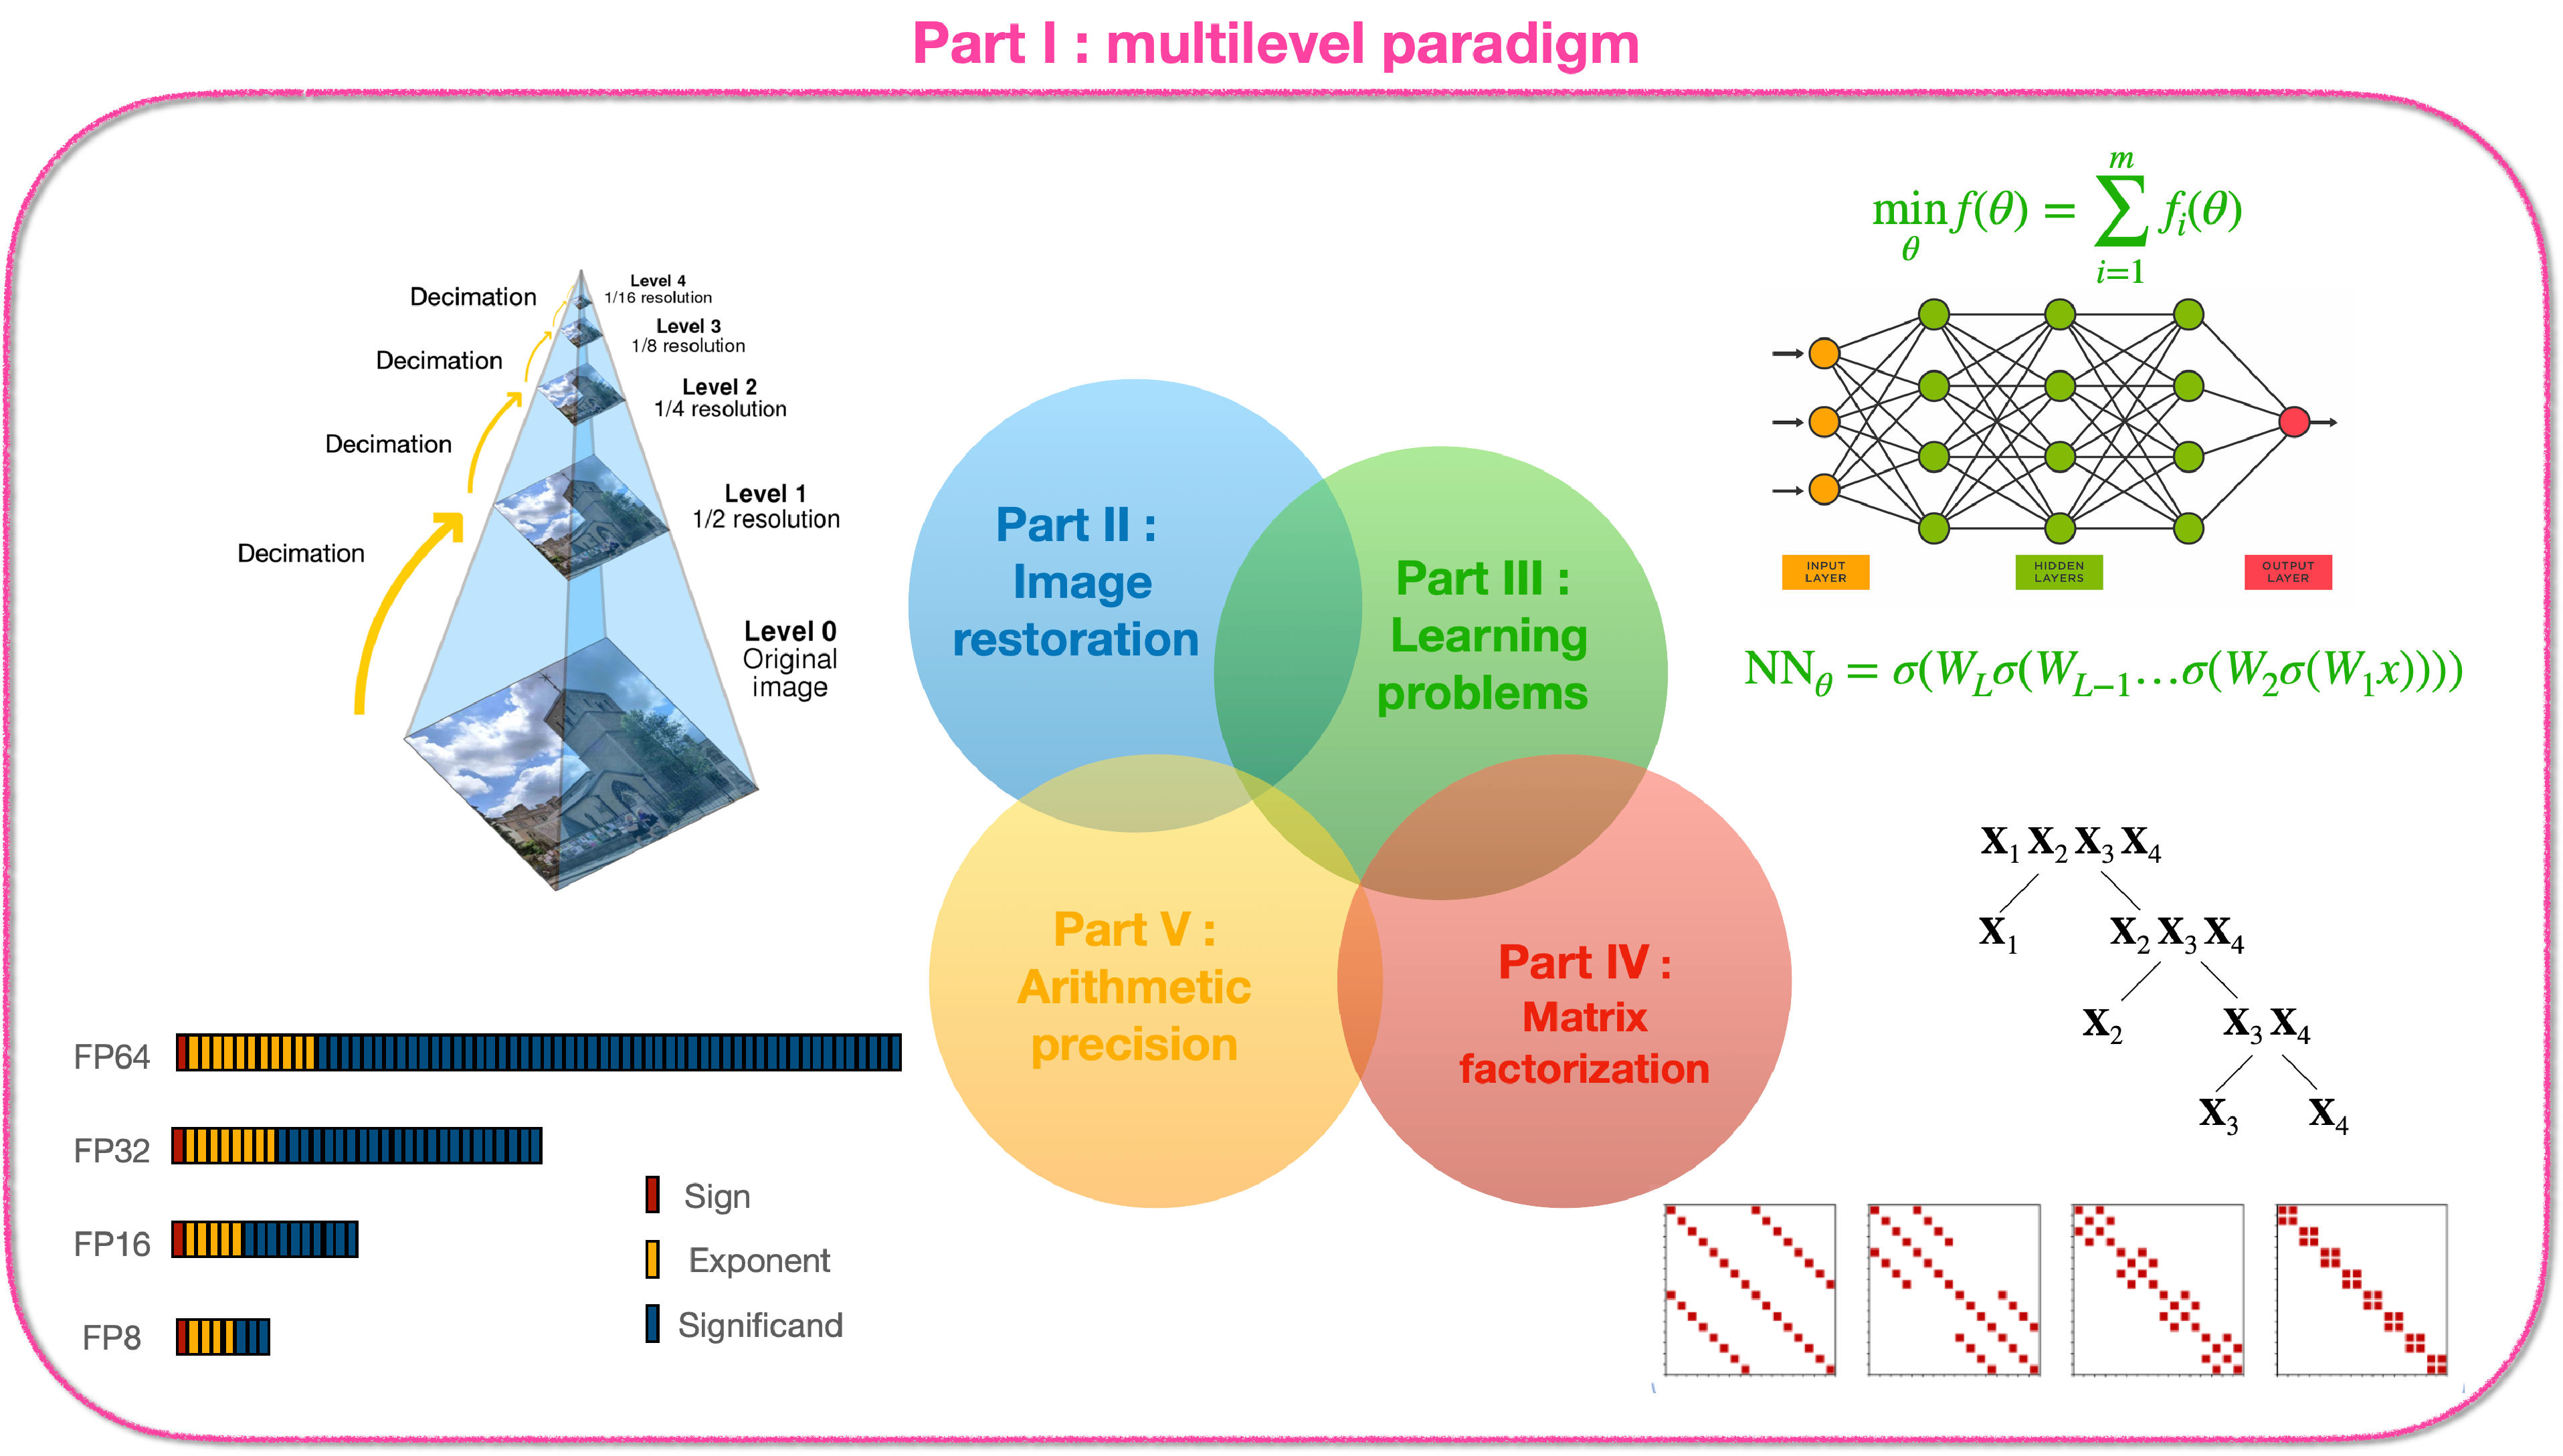
\includegraphics[scale=0.17]{figures/WPs.pdf}
\end{figure}


  \end{frame}
  
 
  
  



\part{The multilevel paradigm}
\frame[plain]{\partpage}

\begin{frame}{Numerical solution of linear PDEs}







\begin{minipage}[t]{0.48\linewidth}
%Given $f :\Omega\subset\mathbb{R}^d\rightarrow\mathbb{R}$, $g :\partial\Omega\rightarrow\mathbb{R}$ and a linear differential operator $D$, find $u:\mathbb{R}^d\rightarrow \mathbb{R}$ that solves
\begin{align*}
D(u(x))=f(x) \text{ in  } \Omega\\
u(x)=g(x) \text{ in  } \partial\Omega
\end{align*}
\centering
$$
\downarrow 
$$
Discretization
$$
\downarrow 
$$

Linear system 
$$
Au=f
$$

\end{minipage}\hfill
\begin{minipage}[t]{0.48\linewidth}

\begin{figure}
    \centering
    \includegraphics[width=0.8\linewidth]{images/grid2.png}
    \caption{Example: d=2, $\Omega=[0,1]\times[0,1]$
}
\end{figure}
 The size of the grid impacts:
 \begin{itemize}
 \item  the \alert{size} of the discrete problem
 \item the  \alert{accuracy} of the solution approximation
 \end{itemize}

\end{minipage}
\end{frame}











 












\begin{comment}
\begin{frame}{Multigrid methods}

{\bf Aim:} accelerate fixed point methods by exploiting multiple grids  \begin{columns}
\begin{column}{0.5\textwidth}
    \begin{figure}
    \centering
    
\includegraphics[width=0.90\linewidth]{images/MG.png}
\end{figure}
\end{column}
\begin{column}{0.40\textwidth}
    \begin{itemize}
\item \underline{Fine scales}: eliminate {\color{red}high frequency} components of the error
\item \underline{Coarse scales}: eliminate {\color{red}low frequency} components of the error
\end{itemize}
\end{column}
\end{columns}


\end{frame}
\end{comment}


\begin{frame}{Multigrid methods}

{\bf Aim:} accelerate fixed point methods by exploiting multiple grids  
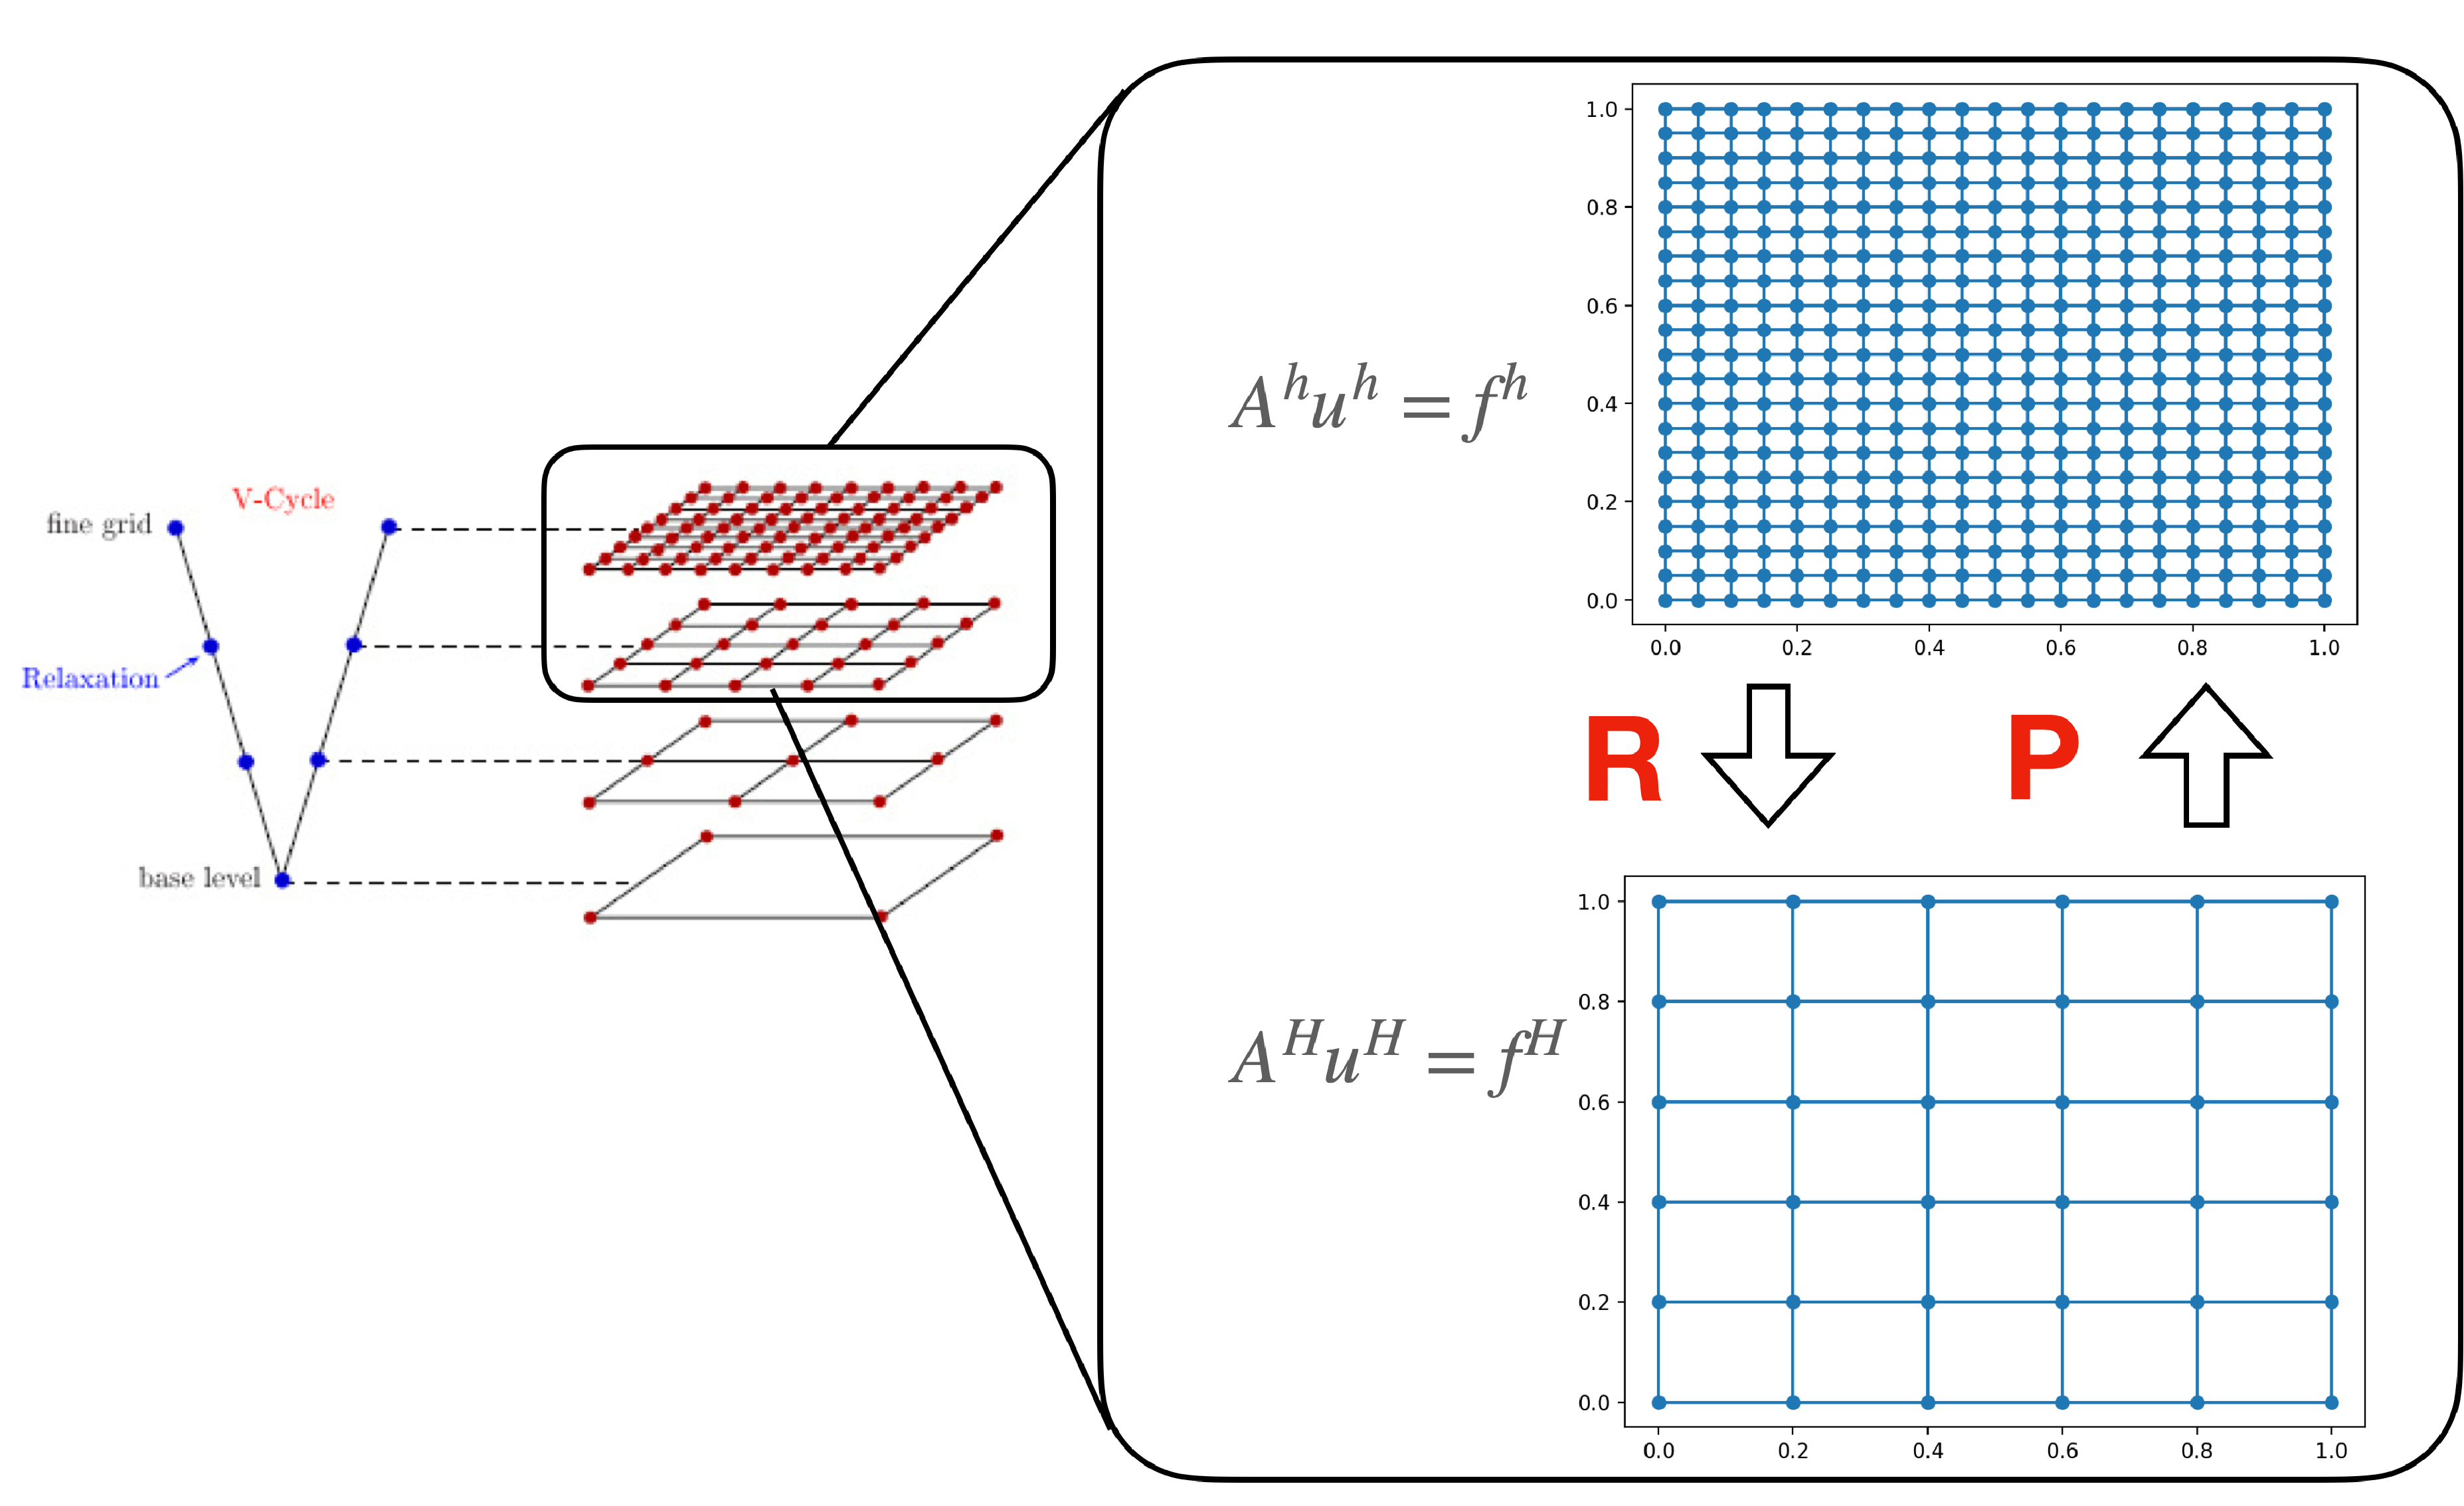
\includegraphics[width=\textwidth]{figures/MG}
\end{frame}


\begin{comment}
\begin{frame}{Multigrid ingredients}
\begin{enumerate}
\item Transfer operators
\begin{columns}
\begin{column}{0.5\textwidth}
Prolongation
\vspace{1cm}
%Build operators to transfer the information between the two levels
\begin{minipage}[t]{\linewidth}

 Interpolation

\begin{align*}
v_{2j}^h&=v_j^{2h}\\
v_{2j+1}^h&=\frac{1}{2}(v_j^{2h}+v_{j+1}^{2h})
\end{align*}
\begin{figure}
    \centering
    \includegraphics[width=0.7\linewidth]{images/P.png}
\end{figure}



\end{minipage}
\end{column}
\begin{column}{0.5\textwidth}
Restriction

%Build operators to transfer the information between the two levels
\begin{minipage}[t]{\linewidth}
\begin{itemize}
\item Injection:
$$
v_j^{2h}=v_{2j}^h
$$
\item Full weighting
$$
v_j^{2h}=\frac{1}{4} (v_{2j-1}^h+2v_{2j}^h+v_{2j+1}^h)
$$
\begin{figure}
    \centering
    \includegraphics[width=0.7\linewidth]{images/R.png}
\end{figure}
\end{itemize}

\end{minipage}

\end{column}
\end{columns}


\item $A^H$: discretization of differential operator on the coarse grid or 
\alert{Galerkin approximation}:
$$
A^{2h}=I_{h}^{2h}A^hI_{2h}^h
$$
\end{enumerate}
    
   % When $A_h=A_H$ the residual equation simplifies:
    %$$
    %A_H(v_H+e_H^N)=R f_h
    %$$

\end{frame}
\end{comment}

\begin{comment}
\begin{frame}{How to define the coarse level operator $A^{2h}$?}
Let  $v^h$  be a computed approximation to the exact solution $u^h$. 
Let  $e^h = u^h - v^h$ and assume that it lies entirely
in the range of interpolation: it exists  $u^{2h}\in\Omega^{2h}$ such that $e^h = I_{2h}^h u^{2h}$. The residual equation becomes:
$$
A^he^h=A^hI_{2h}^hu^{2h}=r^h
$$
We can see that
$A^hI_{2h}^hu^{2h}$ is zero at the odd points of $\Omega^h$, we can obtain $A^{2h}$ by dropping the odd rows, and we can do this by applying the restriction operator to both sides:
$$
I_{h}^{2h}A^hI_{2h}^h u^{2h}=I_{h}^{2h}r^h
$$
A plausible definition is thus 
$$
A^{2h}=I_{h}^{2h}A^hI_{2h}^h,
$$
the \alert{Galerkin condition}.
%We would get the same result if the original problem were simply discretized on Ω2h using the usual second-order finite differences. Therefore, by this definition, A2h really is the Ω2h version of Ah.
%The preceding argument was based on the assumption that the error eh lies entirely in the range of interpolation. This is not the case in general. If it were, then solving the Ω2h residual equation exactly and doing the two-grid correction would give the exact solution. Nevertheless, the argument does give a sensible def- inition for A2h. It also leads us to two important properties called the variational
\end{frame}
\end{comment}



















\begin{frame}{From linear to nonlinear: multilevel methods}
	\begin{tcolorbox}[
        %title={\faExclamationTriangle\ Stochastic problems},
    colback=gray!10,
    colframe=gray!70!black,
        fonttitle=\bfseries,
]


$$
	\min_{x\in\mathbb{R}^n}f(x)
	$$
	 \end{tcolorbox}
	%Classical \alert{iterative} optimization methods:
	\begin{itemize}
	\item Build a \alert{model} ($B_k\approx \nabla^2 f(x_k)$ or $B_k=0$):
	\begin{equation*}
	f(x_k+s)\simeq T_{k}(s)=f(x_k)+s^T\nabla f(x_k)+\frac{1}{2}s^TB_ks
	\end{equation*}
	%with $T_{k}(x_k,s)$ Taylor model, .\\
	\vspace{-0.5cm}
	\item Compute a \alert{step} $s_k$ ($r_k$ regularization term):
	\begin{equation*}
	\underbrace{\min_{s\in\mathbb{R}^{\alert{n}}} m_{k}(s)=T_{k}(s)+r_k(s)}_{\text{bottleneck: subproblem solution}}
	\end{equation*}
	\vspace{-0.5cm}

	\end{itemize}






	
		\vspace{0.5cm}

\pause
\begin{block}{ {\bf Possible solution}:  \alert{multilevel methods} }
		
		\begin{small}
	\begin{itemize}
	\item 
	 \alert{MG/OPT: } \textit{A multigrid approach to discretized optimization problems}, {\color{black} Nash}, {\color{black} 2000}
		\item  \alert{RMTR: } \textit{Recursive trust-region methods}, {\color{black} S. Gratton, A. Sartenaer and  Ph. L. Toint, 2008}
		%\bibitem{E} \textit{On high-order multilevel optimization strategies}, {\color{black} H. Calandra, S. Gratton, E. Riccietti, X. Vasseur}, {\color{black} 2020}

	\end{itemize}
	\end{small}


	\end{block}		
\end{frame}



	
	
	
			
	\begin{frame}\frametitle{Hierarchy of problems {\small ($n_{\ell_{\max}}> n_{\ell_{\max}-1} > \dots >n_0$)}}
{\footnotesize
 \begin{columns}
  \begin{column}{0.2\textwidth}
 \includegraphics[width=0.9\textwidth]{grid-14.mps}    
\end{column}
\begin{column}{0.6\textwidth}
      \begin{block}{} \centerline{$\smash{\mbox{Finest Level  $f^{\ell_{\max}} : \mathbb{R}^{\color{blue}n_{\ell_{\max}}}\to \mathbb{R}$ }}\vphantom{level}$} \end{block} 
\hspace{2cm}{\color{red} $\downarrow$ $R^{\ell_{\max}}$} \hspace{0.3cm}  \alert{$P^{\ell_{\max}}$ $\uparrow$ }  \end{column}
\begin{column}{0.2\textwidth}
\includegraphics[width=0.9\textwidth]{sol_6.eps}    
   \end{column}
     \end{columns} 
 \begin{columns}
  \begin{column}{0.2\textwidth}
 \includegraphics[width=0.9\textwidth]{grid-13.mps}    
\end{column}
\begin{column}{0.6\textwidth}
      \begin{block}{} \centerline{$\smash{\mbox{Fine Level  $f^{\ell_{\max}-1} : \mathbb{R}^{\color{blue}n_{\ell_{\max}-1}}\to \mathbb{R}$ }}\vphantom{level}$} \end{block}  
\hspace{2cm}{\color{red} $\downarrow$ $R^{\ell_{\max}-1}$} \hspace{0.3cm}  \alert{$P^{\ell_{\max}-1}$ $\uparrow$ } 
\end{column}
\begin{column}{0.2\textwidth}
 \includegraphics[width=0.9\textwidth]{unc_sol.eps}    
   \end{column}
     \end{columns} 

\begin{columns}
  \begin{column}{0.2\textwidth}
  \end{column}
\begin{column}{0.6\textwidth}
     \begin{block}{} \centerline{$\smash{\vdots}\vphantom{level}$} \end{block}  
\hspace{2cm}{\color{red} $\downarrow$ $R^{2}$}\hspace{1cm}  \alert{$P^{2}$ $\uparrow$ } 
  \end{column}
\begin{column}{0.2\textwidth}
   \end{column}
     \end{columns} 

 \begin{columns}
  \begin{column}{0.2\textwidth}
 \includegraphics[width=0.9\textwidth]{grid-12.mps}    
\end{column}
\begin{column}{0.6\textwidth}
      \begin{block}{} \centerline{$\smash{\mbox{Coarse Level  $f^2 : \mathbb{R}^{\color{blue}n_2}\to \mathbb{R}$ }}\vphantom{level}$} \end{block} 
\hspace{2cm}{\color{red} $\downarrow$ $R^1$} \hspace{1cm}  \alert{$P^{1}$ $\uparrow$ }  \end{column}
\begin{column}{0.2\textwidth}
\includegraphics[width=0.9\textwidth]{sol_2.eps}    
   \end{column}
     \end{columns} 
 \begin{columns}
  \begin{column}{0.2\textwidth}
 \includegraphics[width=0.9\textwidth]{grid-11.mps}    
\end{column}
\begin{column}{0.6\textwidth}
      \begin{block}{} \centerline{$\smash{\mbox{Coarsest Level  $f^0 : \mathbb{R}^{\color{blue}n_0}\to \mathbb{R}$ }}\vphantom{level}$} \end{block} 
 \end{column}
\begin{column}{0.2\textwidth}
\includegraphics[width=0.9\textwidth]{sol_1.eps}    
   \end{column}
     \end{columns} 
}


\end{frame}


		
		
\begin{comment}
\begin{frame}{Classical one-level method}

Let $x_k$ be the current approximation. 

We look for $s_k$ to define the new approximation

\begin{center}
		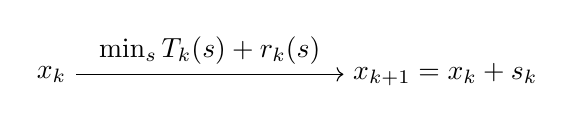
\begin{tikzpicture}[scale=2]
		\node(a) at (0,1){$x_k$};
		\pause
		 		\node(d) at (2.5,1){$x_{k+1} = x_k+s_k$};
		\draw (a) edge[->] node[above]{$\min_{s} T_k(s)+r_k(s)$} (d);
	\end{tikzpicture}
	\end{center}


\end{frame}
\begin{frame}{Multilevel strategy}
 % \vspace{-0.2cm}
	\begin{block}{Hierarchy of problems}
		\begin{itemize}
      \item $\{f^h(x^h)\}$, $x^h\in\mathbb{R}^{n_h}$
      \item \alert{$n_{H} < n_h$} $\Raw$ $f^{H}$ is cheaper to optimize compared with $f^h$
      \item $\mu^{H}$ model for $f^{H}$
		\end{itemize}
	\end{block}
	\end{frame}
	
	\begin{frame}{Multilevel strategy: step computation }
	
	Two choices:
	\begin{enumerate}
	\item \alert{Classical fine step}
	\item Coarse step
		\end{enumerate}
		
	\begin{center}
		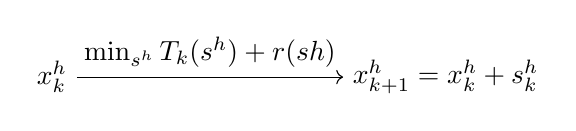
\begin{tikzpicture}[scale=2]
		\node(a) at (0,1){$x_k^h$};
		 		\node(d) at (2.5,1){$x_{k+1}^h = x_k^h+s_k^h$};

		\draw (a) edge[->] node[above]{$\min_{s^h} T_k(s^h)+r(sh)$} (d);

		 
		
		\end{tikzpicture}
	\end{center}
	

	
	
\end{frame}


\begin{frame}{Multilevel strategy}
 
	Two choices:
	\begin{enumerate}
	\item Classical fine step
	\item \alert{Coarse step}
		\end{enumerate}

	\begin{center}
		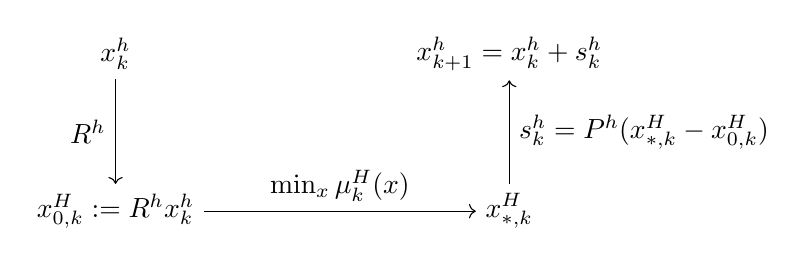
\begin{tikzpicture}[scale=2]
		\node(a) at (0,1){$x_k^h$};
		 
		\node(b) at (0,0){$x_{0,k}^{H} := R^h x_k^h$};
		\draw (a) edge[->] node[left]{$R^h$} (b);
		 
		\node(c) at (2.5,0){$x_{*,k}^{H}$};
		\draw (b) edge[->] node[above]{$\min_x \mu_k^{H}(x)$}(c);
		 
		\node(d) at (2.5,1){$x_{k+1}^h = x_k^h+s_k^h$};
		\draw (c) edge[->] node[right]{$s_k^h=P^h(\alert{x_{*,k}^{H}-x_{0,k}^{H}})$} (d);
		
		\end{tikzpicture}
	\end{center}
	

	
	
\end{frame}

\end{comment}


\begin{frame}{Classical one-level method: step computation}

		
	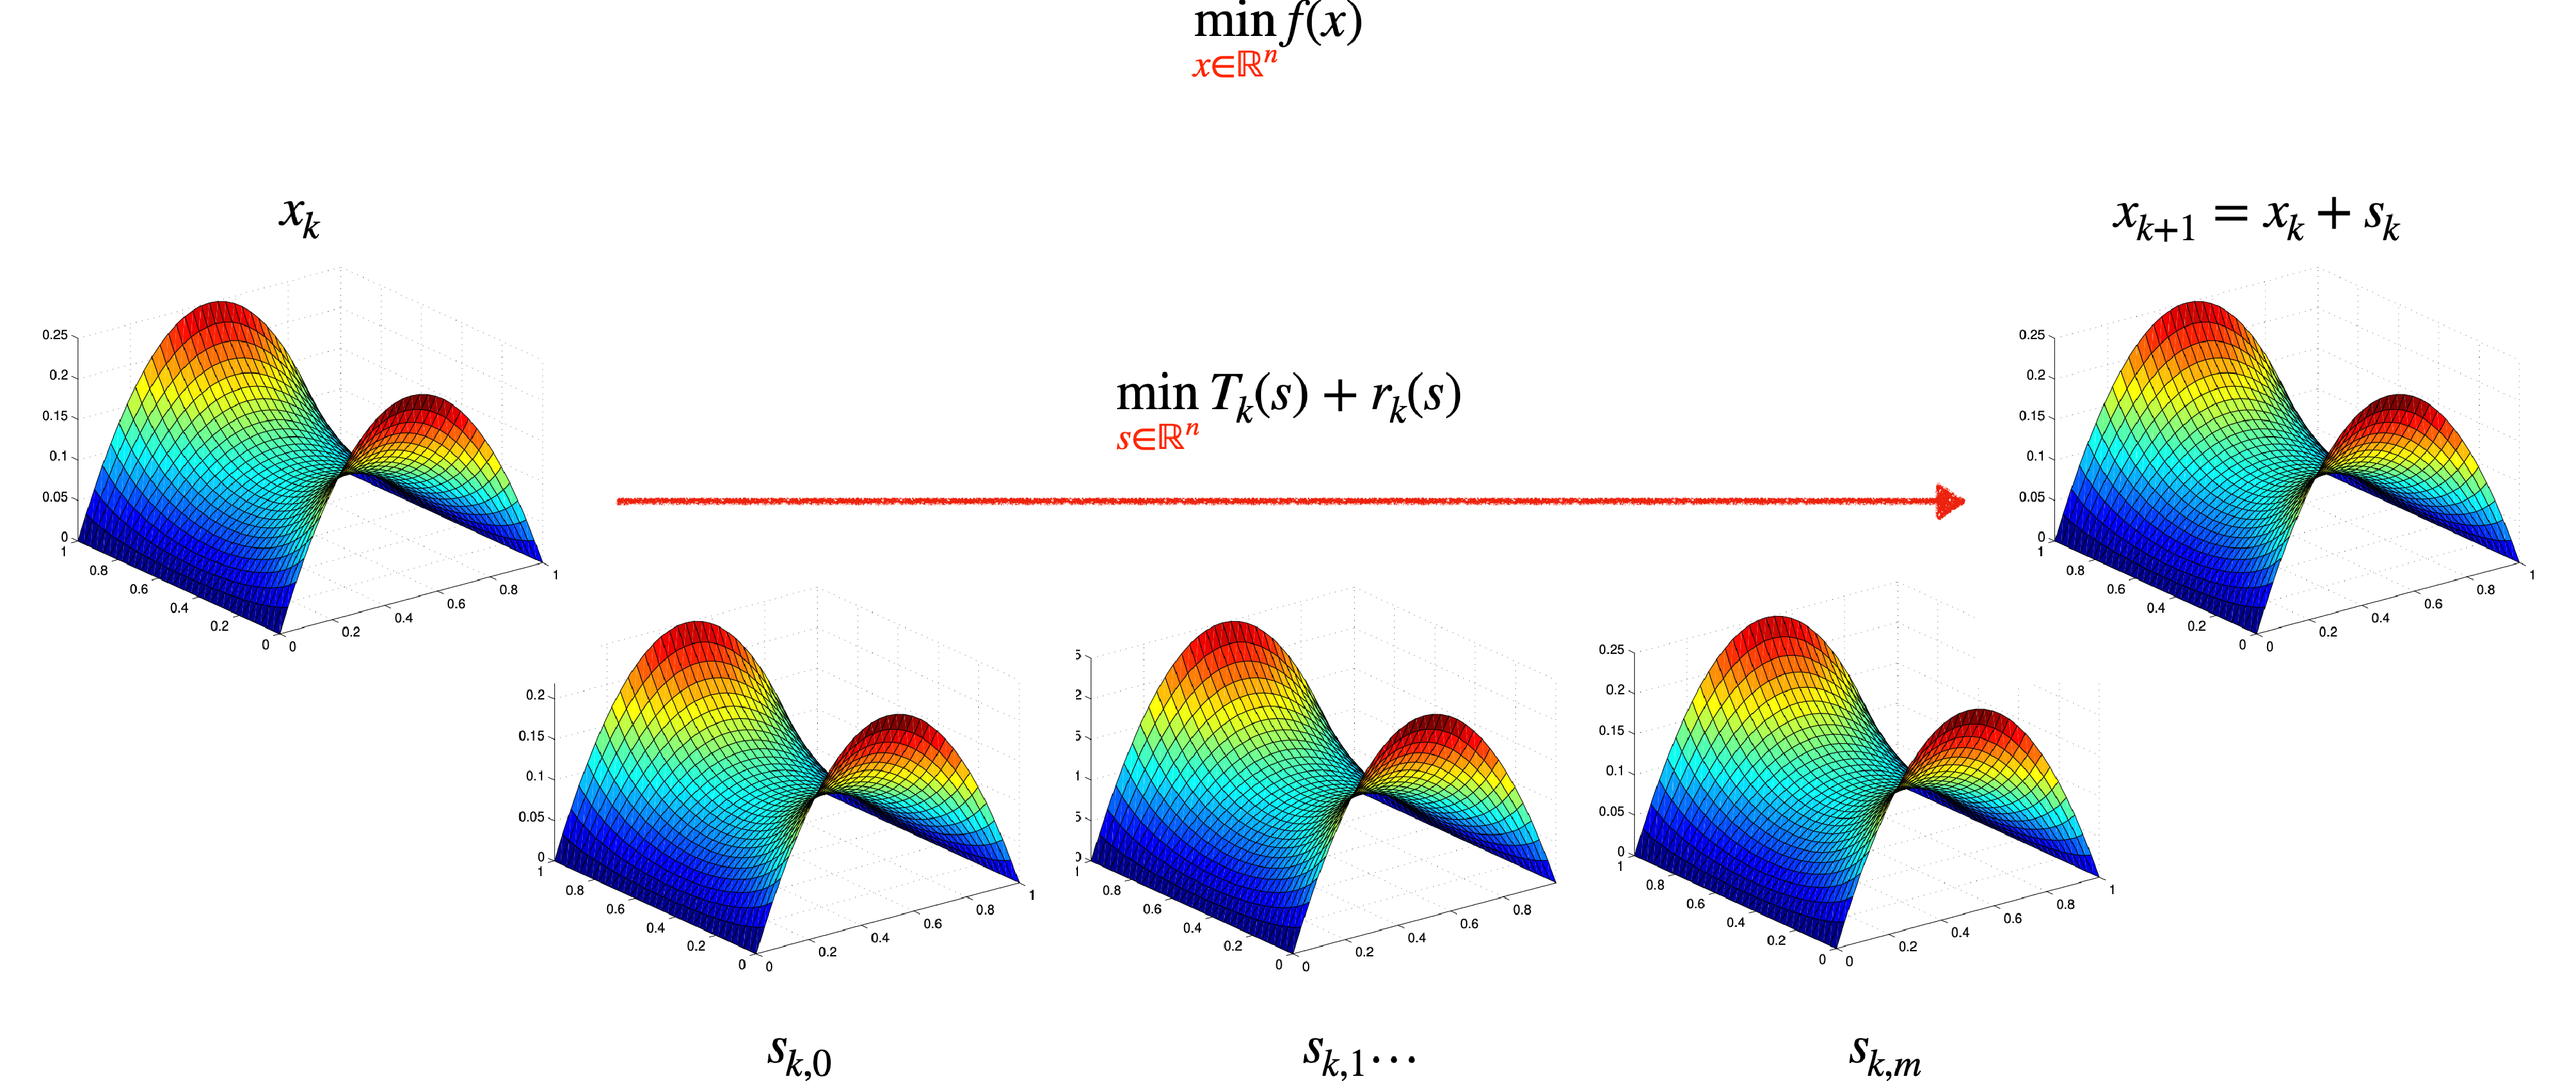
\includegraphics[width=\textwidth]{figures/iter_fine2}
\end{frame}

\begin{frame}{Multilevel strategy: step computation }
	
	
%\includegraphics[width=\textwidth]{scheme_iter}
		

		
	%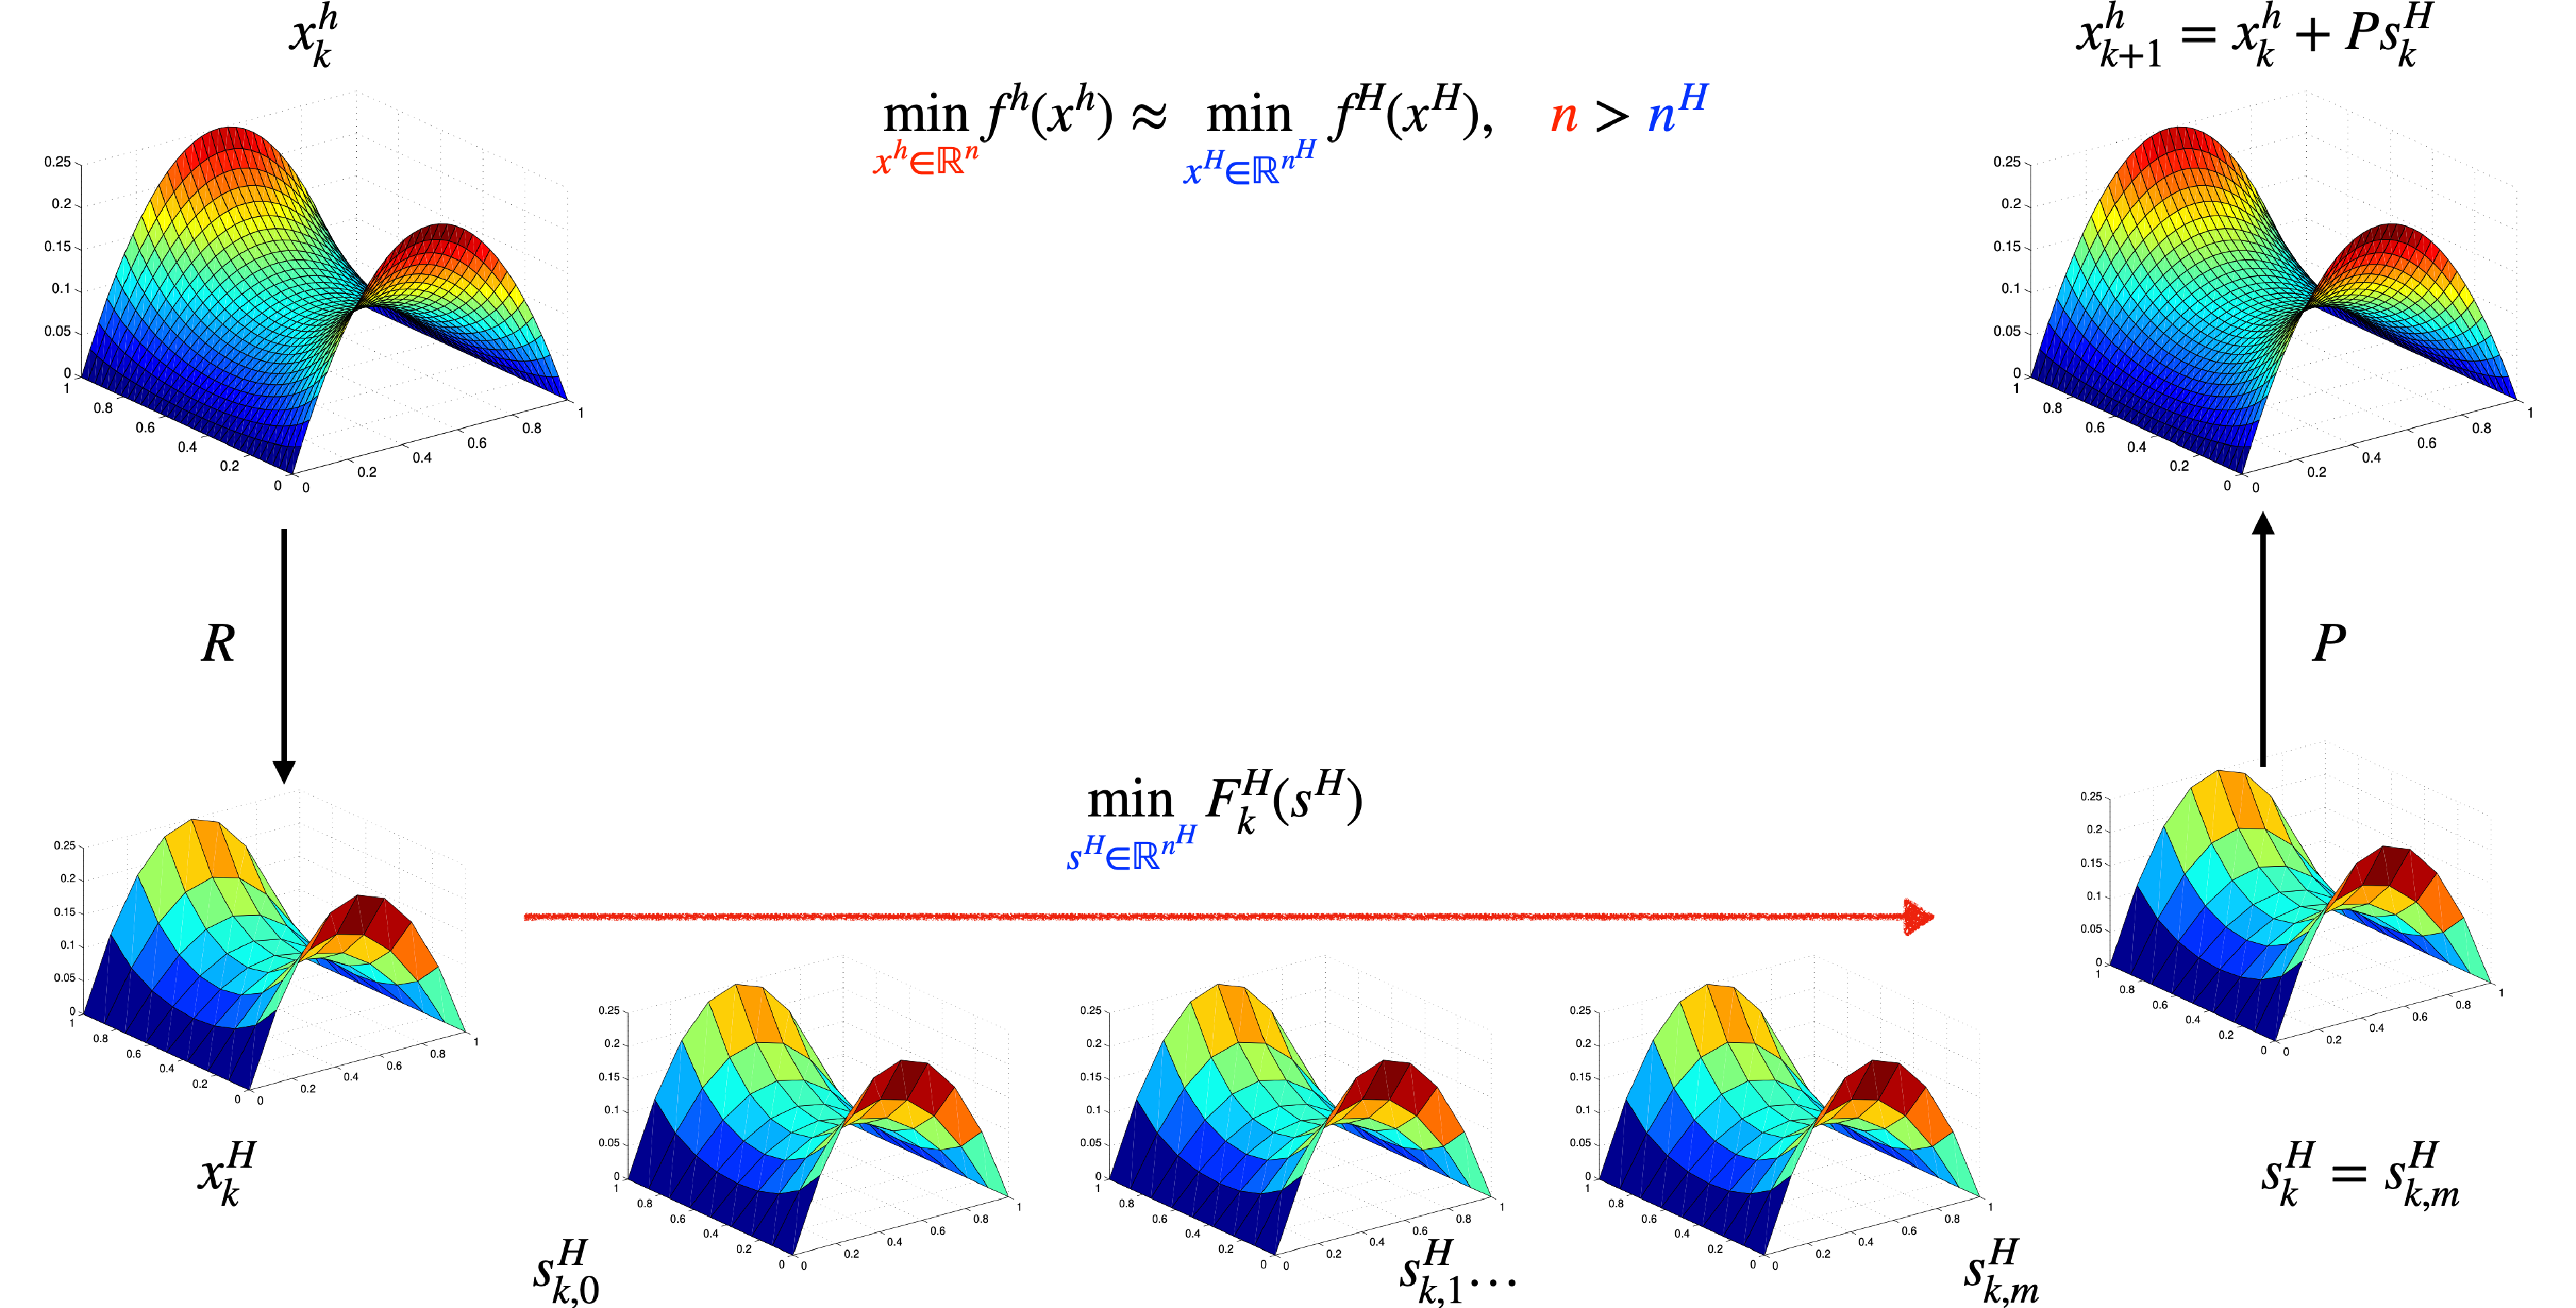
\includegraphics[width=\textwidth]{figures/ML_step2}
		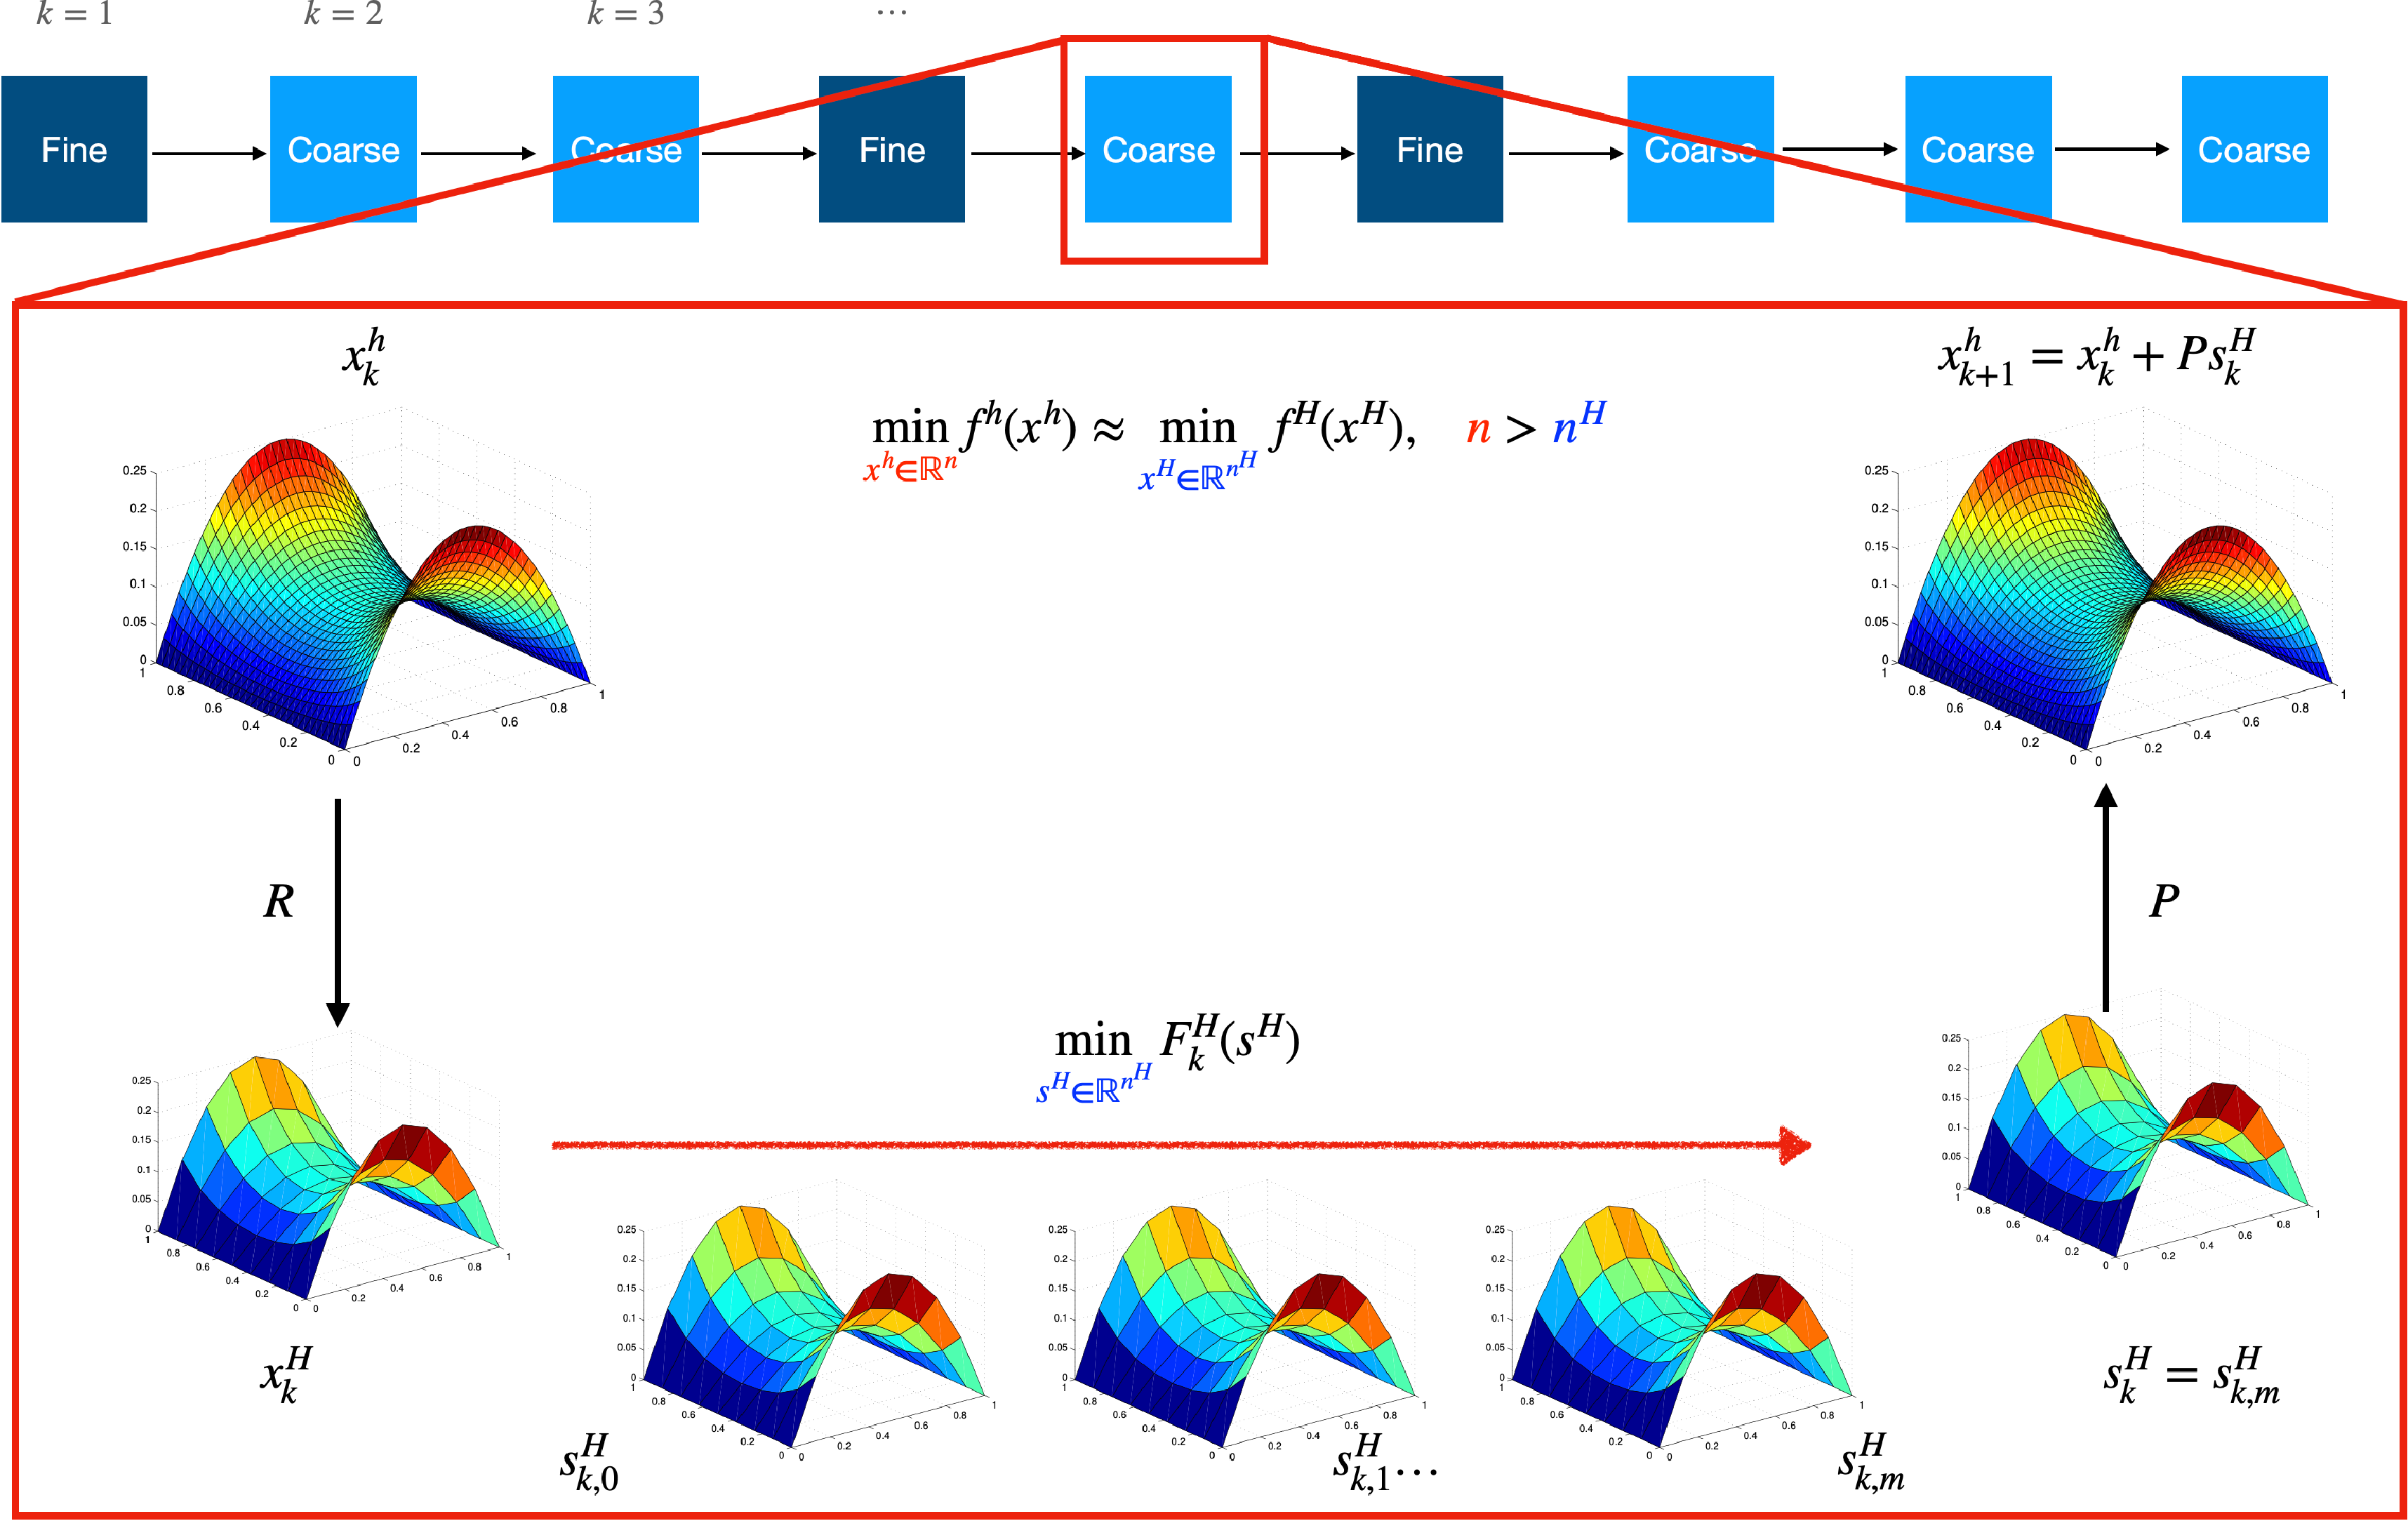
\includegraphics[width=\textwidth]{figures/coarse_step}

\end{frame}


%\begin{frame}{An iteration of a multilevel procedure - two-levels}
%\centering
%\includegraphics[height = 6cm]{images/kiter}
%\pause 
%\alert{$R,P$?} \hspace{5cm} \alert{$F_H$?}
%\end{frame}





		
	
\begin{comment}
\begin{frame}{Definition of lower level model: first-order coherence}
    %\includesvg[width = 0.5\textwidth]{images/slide_first_order_coherence/First_order_coherence.svg}
    \centering
   % \includegraphics[width = 1\textwidth]{images/slide_first_order_coherence/figure-presentation_multiniveau_bonnesdimensions.pdf}
      %  
\includegraphics[width = 1\textwidth]{../../projects/HDR/figures/correction2.pdf}
                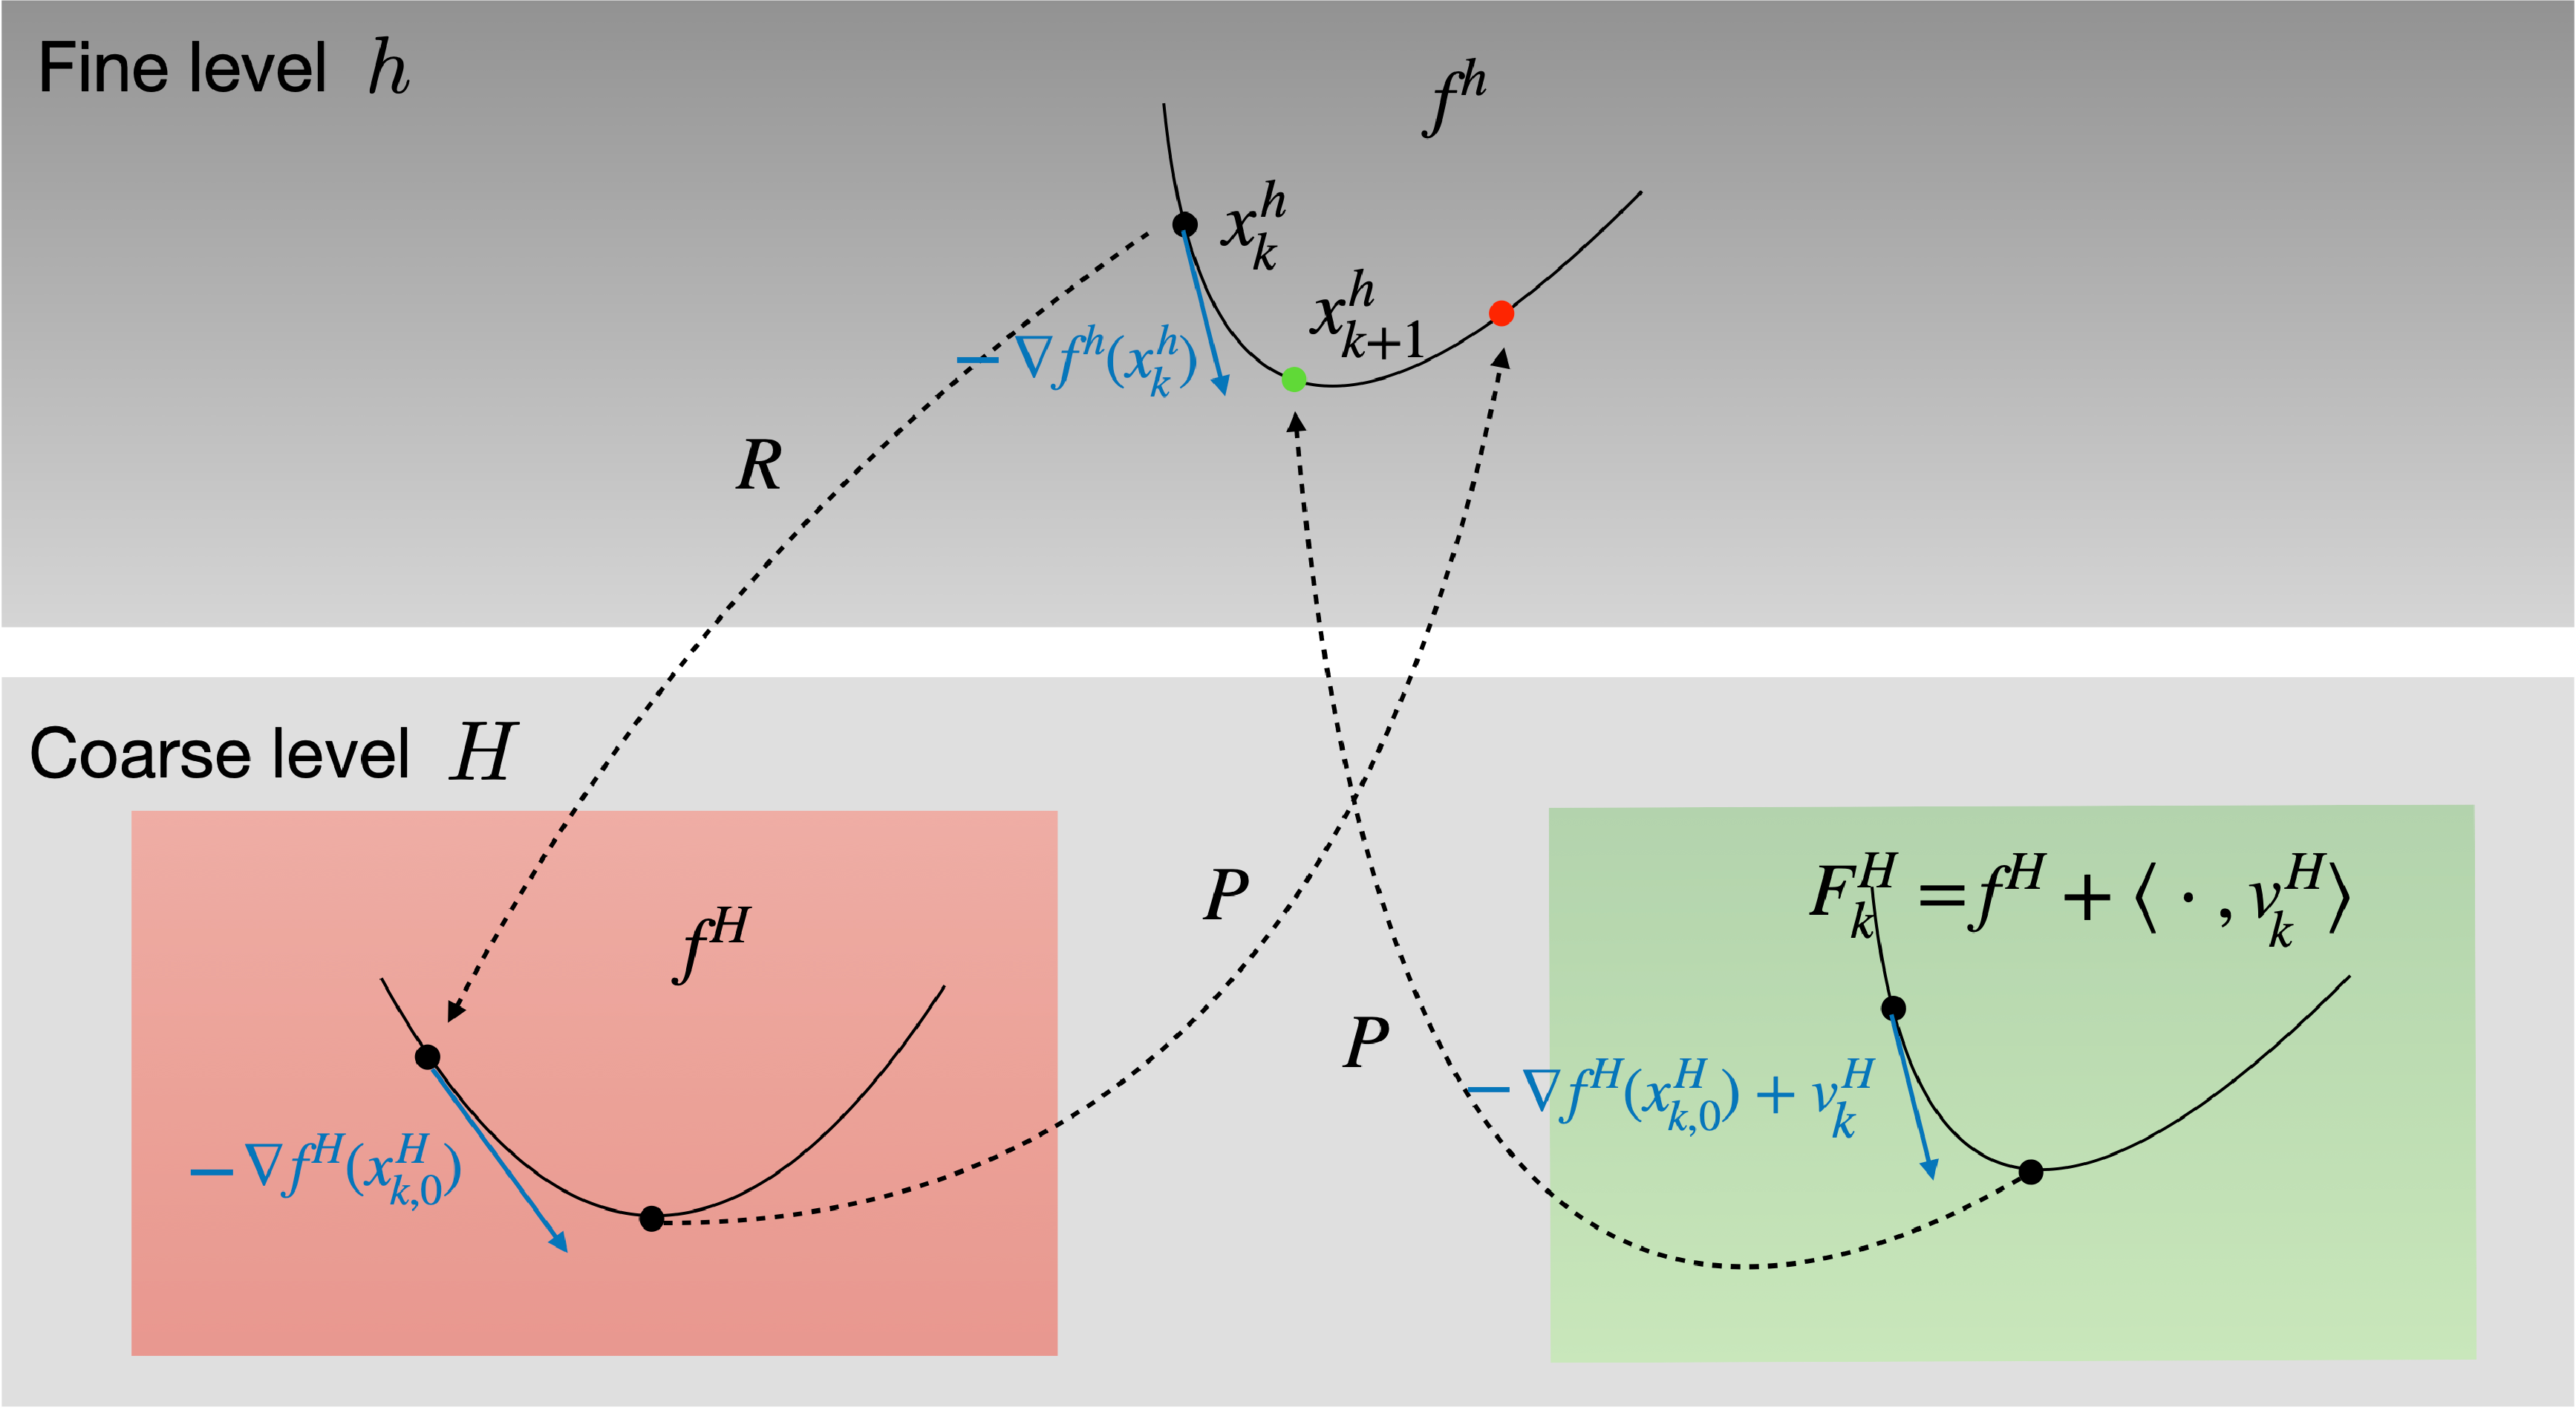
\includegraphics[width = 1\textwidth]{figures/correction2.pdf}


   $v_k^{H}=R\nabla f^h(x_k^{h})-\nabla f^{H} (x_k^{H})\rightarrow \underbrace{\nabla F_{k}^{H}(0^{H})=R\nabla f^h(x_k^h)}_{\text{first-order coherence}}$
\end{frame}
\end{comment}

			










	


	

	

\begin{frame}{My contributions (I): multilevel adaptive regularization  }





	\begin{tcolorbox}[
	 title=AR$q$:  adaptive regularization methods of order $q\geq 1$,
    colback=gray!15,
    colframe=gray!50,
    arc=3mm,
    boxrule=0pt
]


	
	 
	%Classical \alert{iterative} optimization methods:
	\footnotesize{
	\begin{itemize}
	%\item  Build a model :
	%$\displaystyle
	 %T_{k,\alert{q}}(s)=f(x)+\sum_{i=1}^{\alert{q}}\frac{1}{i!}\nabla_x^i f(x)\left[ s\right]^i.
	 %$
	

	\item  Step computation (\alert{bottleneck!}): $\displaystyle{
	\min_{s\in\mathbb{R}^n} m_{k,\alert{q}}(s)=f(x)+\sum_{i=1}^{\alert{q}}\frac{1}{i!}\nabla_x^i f(x)\left[ s\right]^i+\frac{\lambda_k}{\alert{q+1}}\|s\|^{\alert{q+1}},\quad \lambda_k>0}
$

\item Notable example: \textcolor{myblue}{ARC} (adaptive cubic regularization \textcolor{myblue}{$q=2$})
		$$
		m_{k,2}(s)=f(x_k)+s^T\nabla f(x_k)+\frac{1}{2}s^T\nabla^2f(x_k)s+\textcolor{myblue}{\frac{\lambda_k}{3}\|s\|^{3}}
$$


	\end{itemize}}
\end{tcolorbox}

\vspace{-0.2cm}





			
		

	
{\tiny
\parbox{\linewidth}{%
\textcolor{gray}{%
[Birgin, Gardenghi, Marinez, Santos, and Toint,
%\textbf{Worst-case evaluation complexity for unconstrained nonlinear optimization using high-order regularized models∗}, 
2016],[Cartis, Gould, Toint,
%\textbf{Evaluation Complexity of Algorithms for Nonconvex Optimization: Theory, Computation and Perspectives}, 
2022]}}
}
		
		
				
\vspace{-0.3cm}

		\begin{tcolorbox}[
        title={\faSmile\  Multilevel extension MAR$q$ 
},
    colback=green!10,
    colframe=green!70!black,
        fonttitle=\bfseries,
]

				\begin{itemize}
		\item Global convergence, \underline{local rate of convergence} $\left(\frac{\|x_{k+1}-x^*\|}{\|x_k-x^*\|^q}\leq c, \quad \forall k\geq\bar{k}
\right)$, complexity ($O(\epsilon^{-(q+1)/q})$), simple proofs!
		\end{itemize}



		
		

\end{tcolorbox}

\small{ \textcolor{mygreen}{[Calandra, Gratton, R., Vasseur, SIOPT, 2020]}}


		
\end{frame}


\begin{comment}
\begin{frame}{My contribution (II): stochastic optimization problems}

\begin{columns}
\begin{column}{0.5\textwidth}
	\begin{footnotesize}
\begin{tcolorbox}[
        %title={\faExclamationTriangle\ Stochastic problems},
    colback=gray!10,
    colframe=gray!70!black,
        fonttitle=\bfseries,
]

	$$
	\min_x f(x)
	$$
	where $f$ can only be computed \alert{with some noise}.
	\end{tcolorbox}
	\end{footnotesize}
	\end{column}
\begin{column}{0.5\textwidth}

	
	
	\begin{itemize}
	\item expected risk minimization problems
	\item Monte Carlo simulations
      \end{itemize}

 \end{column}
\end{columns}
 
	\begin{footnotesize}
\begin{tcolorbox}[
        title={\faExclamationTriangle\ Limitations  of existing methods},
    colback=red!10,
    colframe=red!70!black,
        fonttitle=\bfseries,
]
\underline{Stochastic methods}: 
 \begin{itemize}
 \item 
 Accuracy of the function approximations \alert{grows} asymptotically, which leads to iterations that are more and more expensive:
 $$
 \|f(x)-\tilde f(x)\|\leq \epsilon_k, \quad \epsilon_k\rightarrow 0
 $$
  \item Such methods control the accuracy of the function estimates but not the \alert{size of the variables}.   
 \end{itemize}

 
%Challenge: develop \alert{scalable} stochastic methods, able to handle the increasing costs of large scale stochastic optimization problems. 

\underline{Multilevel framework}:
\begin{itemize}
 \item Limited to \alert{deterministic} contexts
 \item Still needs to handle \alert{full problem} at the finest scale
 \end{itemize}


\end{tcolorbox}
\end{footnotesize}
 
  

 \end{frame}
 \end{comment}


 \begin{frame}{My contribution (II): stochastic multilevel iterations}
\begin{columns}
\begin{column}{0.2\textwidth}
	\begin{footnotesize}
\begin{tcolorbox}[
        %title={\faExclamationTriangle\ Stochastic problems},
    colback=gray!10,
    colframe=gray!70!black,
        fonttitle=\bfseries,
]

	$$
	\min_x f(x)
	$$
	with \alert{noisy} $f$  
	\end{tcolorbox}
	\end{footnotesize}
	\end{column}
\begin{column}{0.8\textwidth}
 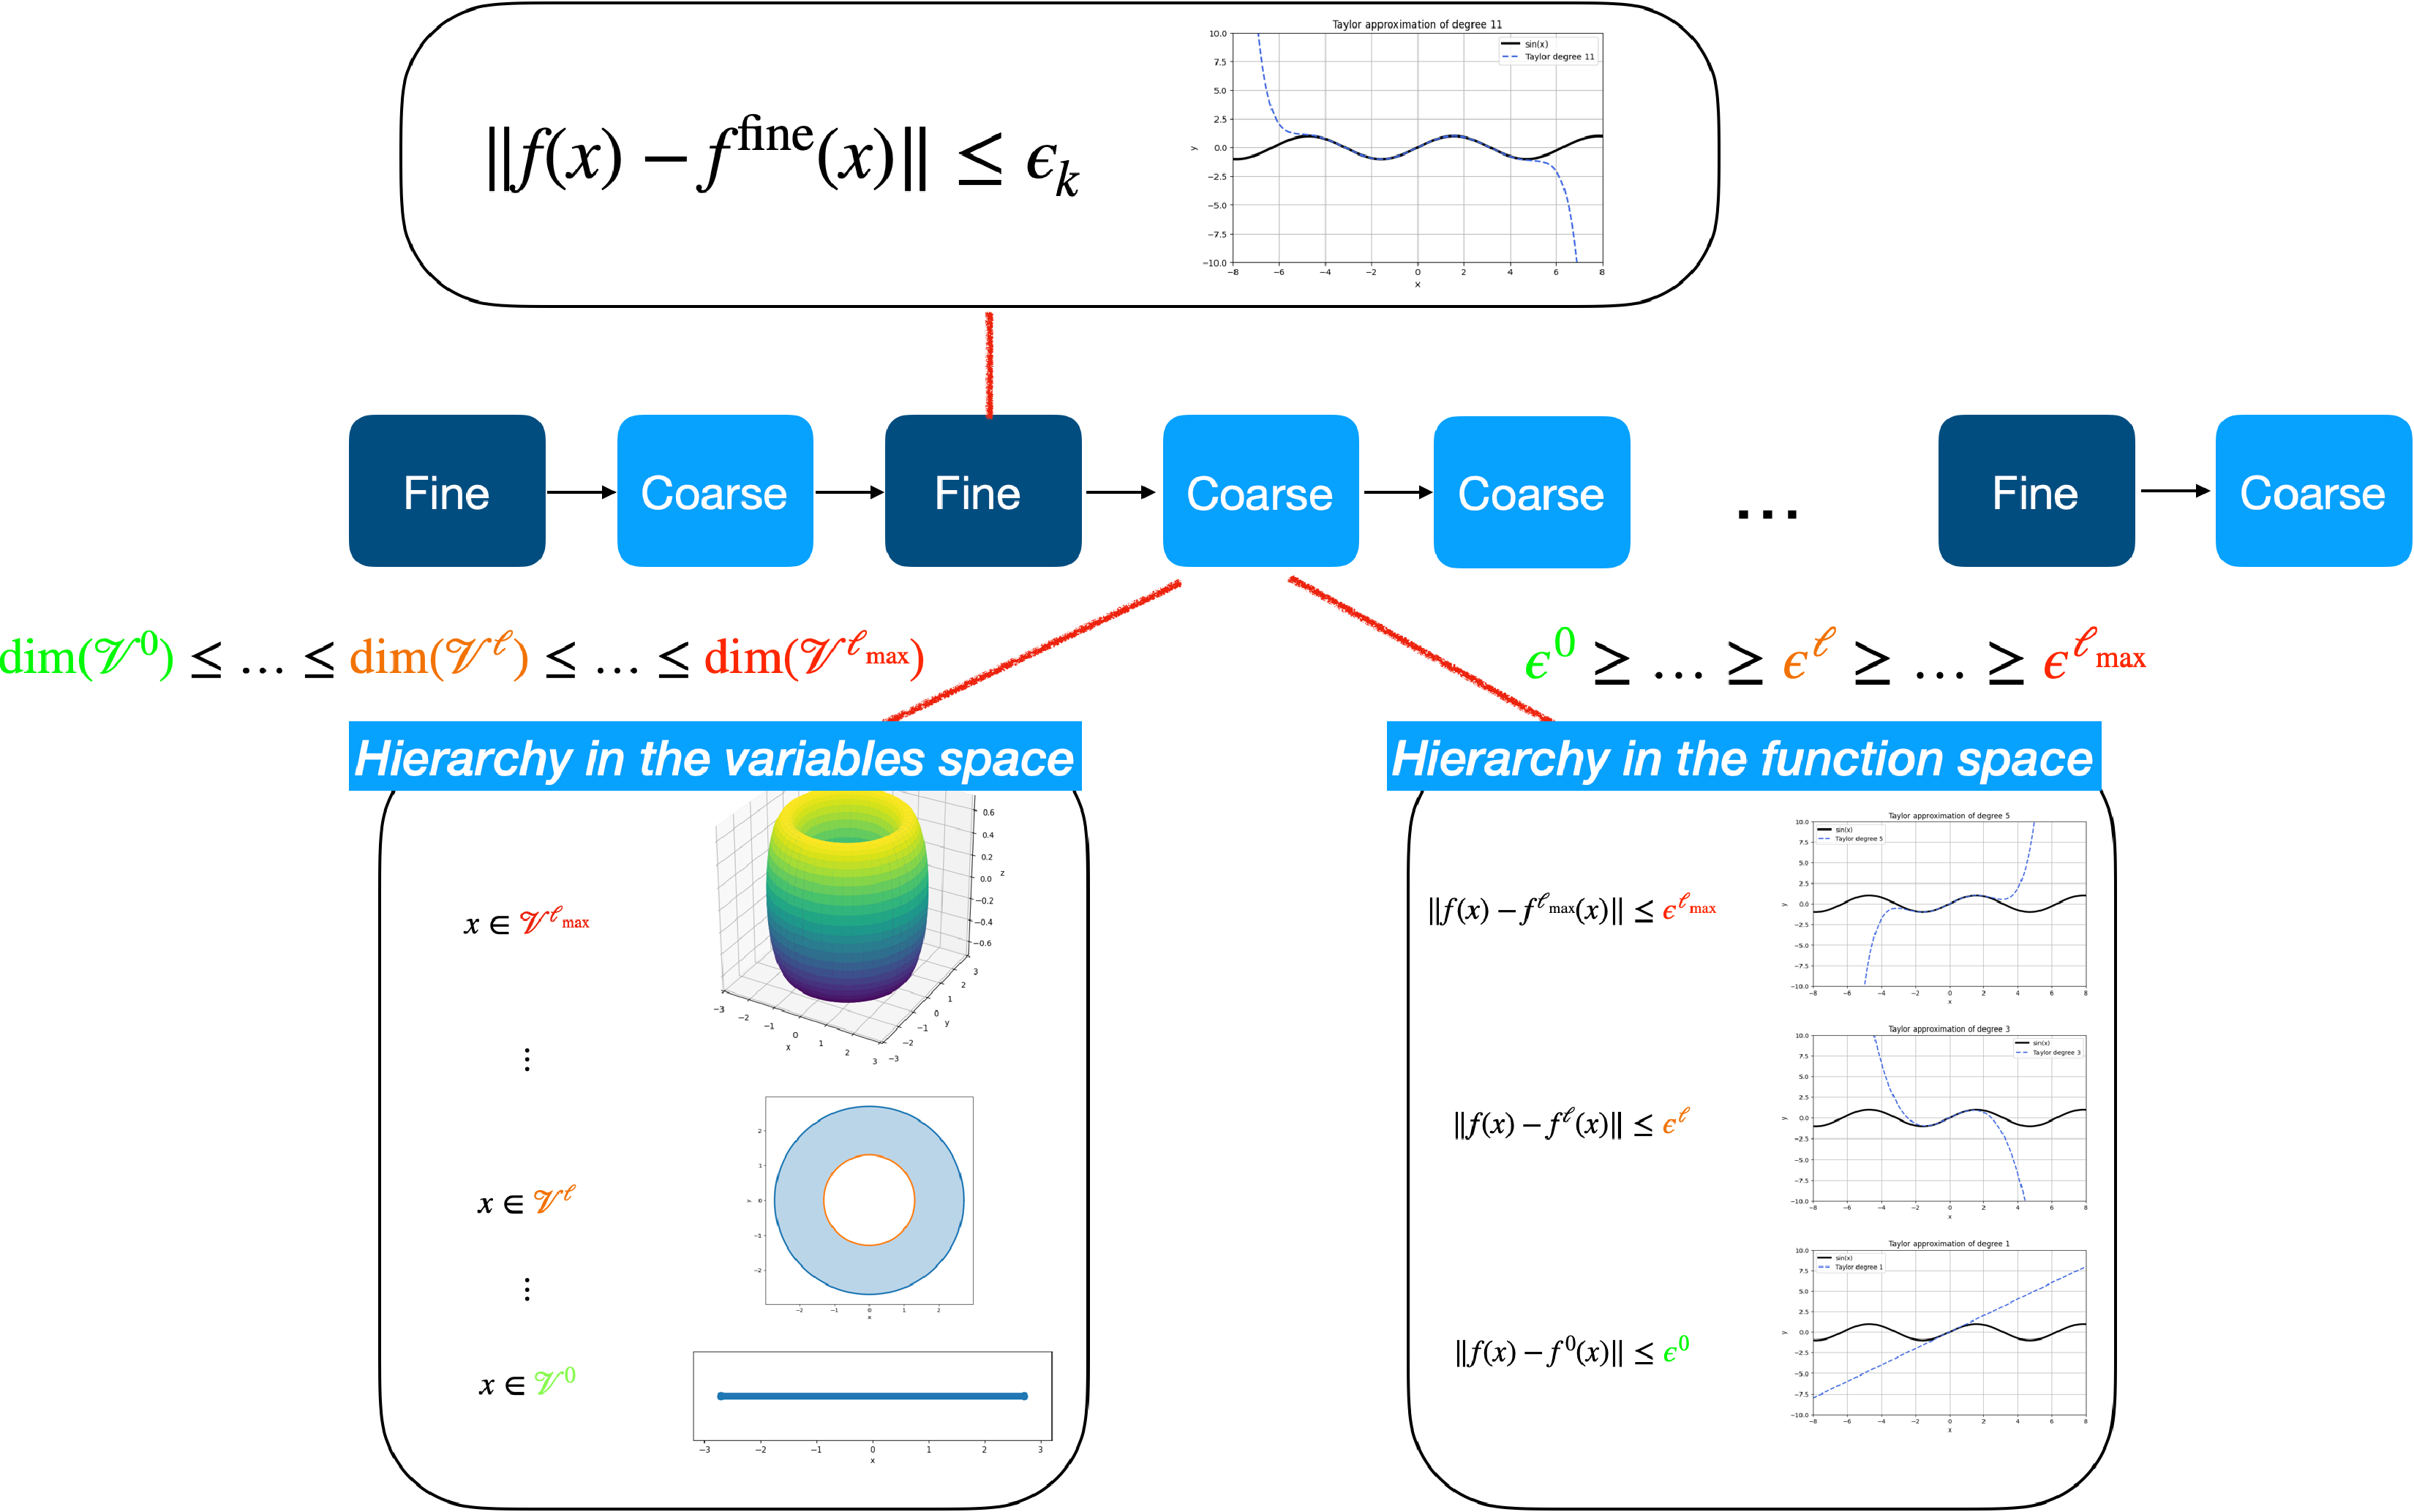
\includegraphics[scale=0.16]{figures/schema_new}
 
\end{column}
\end{columns}
% \begin{tiny} \structure{F. Marini, M. Porcelli,  E. Riccietti, 
  % \textbf{A multilevel stochastic regularized first-order method with application to finite sum minimization}, 2026, accepted in Mathematics of computation}  
%\end{tiny}

\vspace{0.5cm}
Convergence with \alert{probability one} for the stochastic process $\{M_k, X_k, S_k, \Lambda_k, F_k\}$. \small{ \textcolor{mygreen}{[  Marini, Porcelli, R., MathComp, 2026]}}


%\begin{footnotesize}
%	\begin{thebibliography}{9}
%		\setbeamertemplate{bibliography item}[article]
%			\bibitem{E} \textit{A multilevel stochastic regularized first-order method with application to finite sum minimization}, {\color{black} F. Marini, M. Porcelli,  E. Riccietti}, {\color{black} 2026}
%				\end{thebibliography} 
%	\end{footnotesize}
	



 \end{frame}

\begin{frame}{My contribution (II): stochastic multilevel iterations}

	\begin{footnotesize}
\begin{tcolorbox}[
        %title={\faExclamationTriangle\ Stochastic problems},
    colback=gray!10,
    colframe=gray!70!black,
        fonttitle=\bfseries,
]

	$
	\displaystyle{\min_x f(x)}
	$
	where $f$ can only be computed with some  \alert{noise}  
	\end{tcolorbox}
	\end{footnotesize}
	
 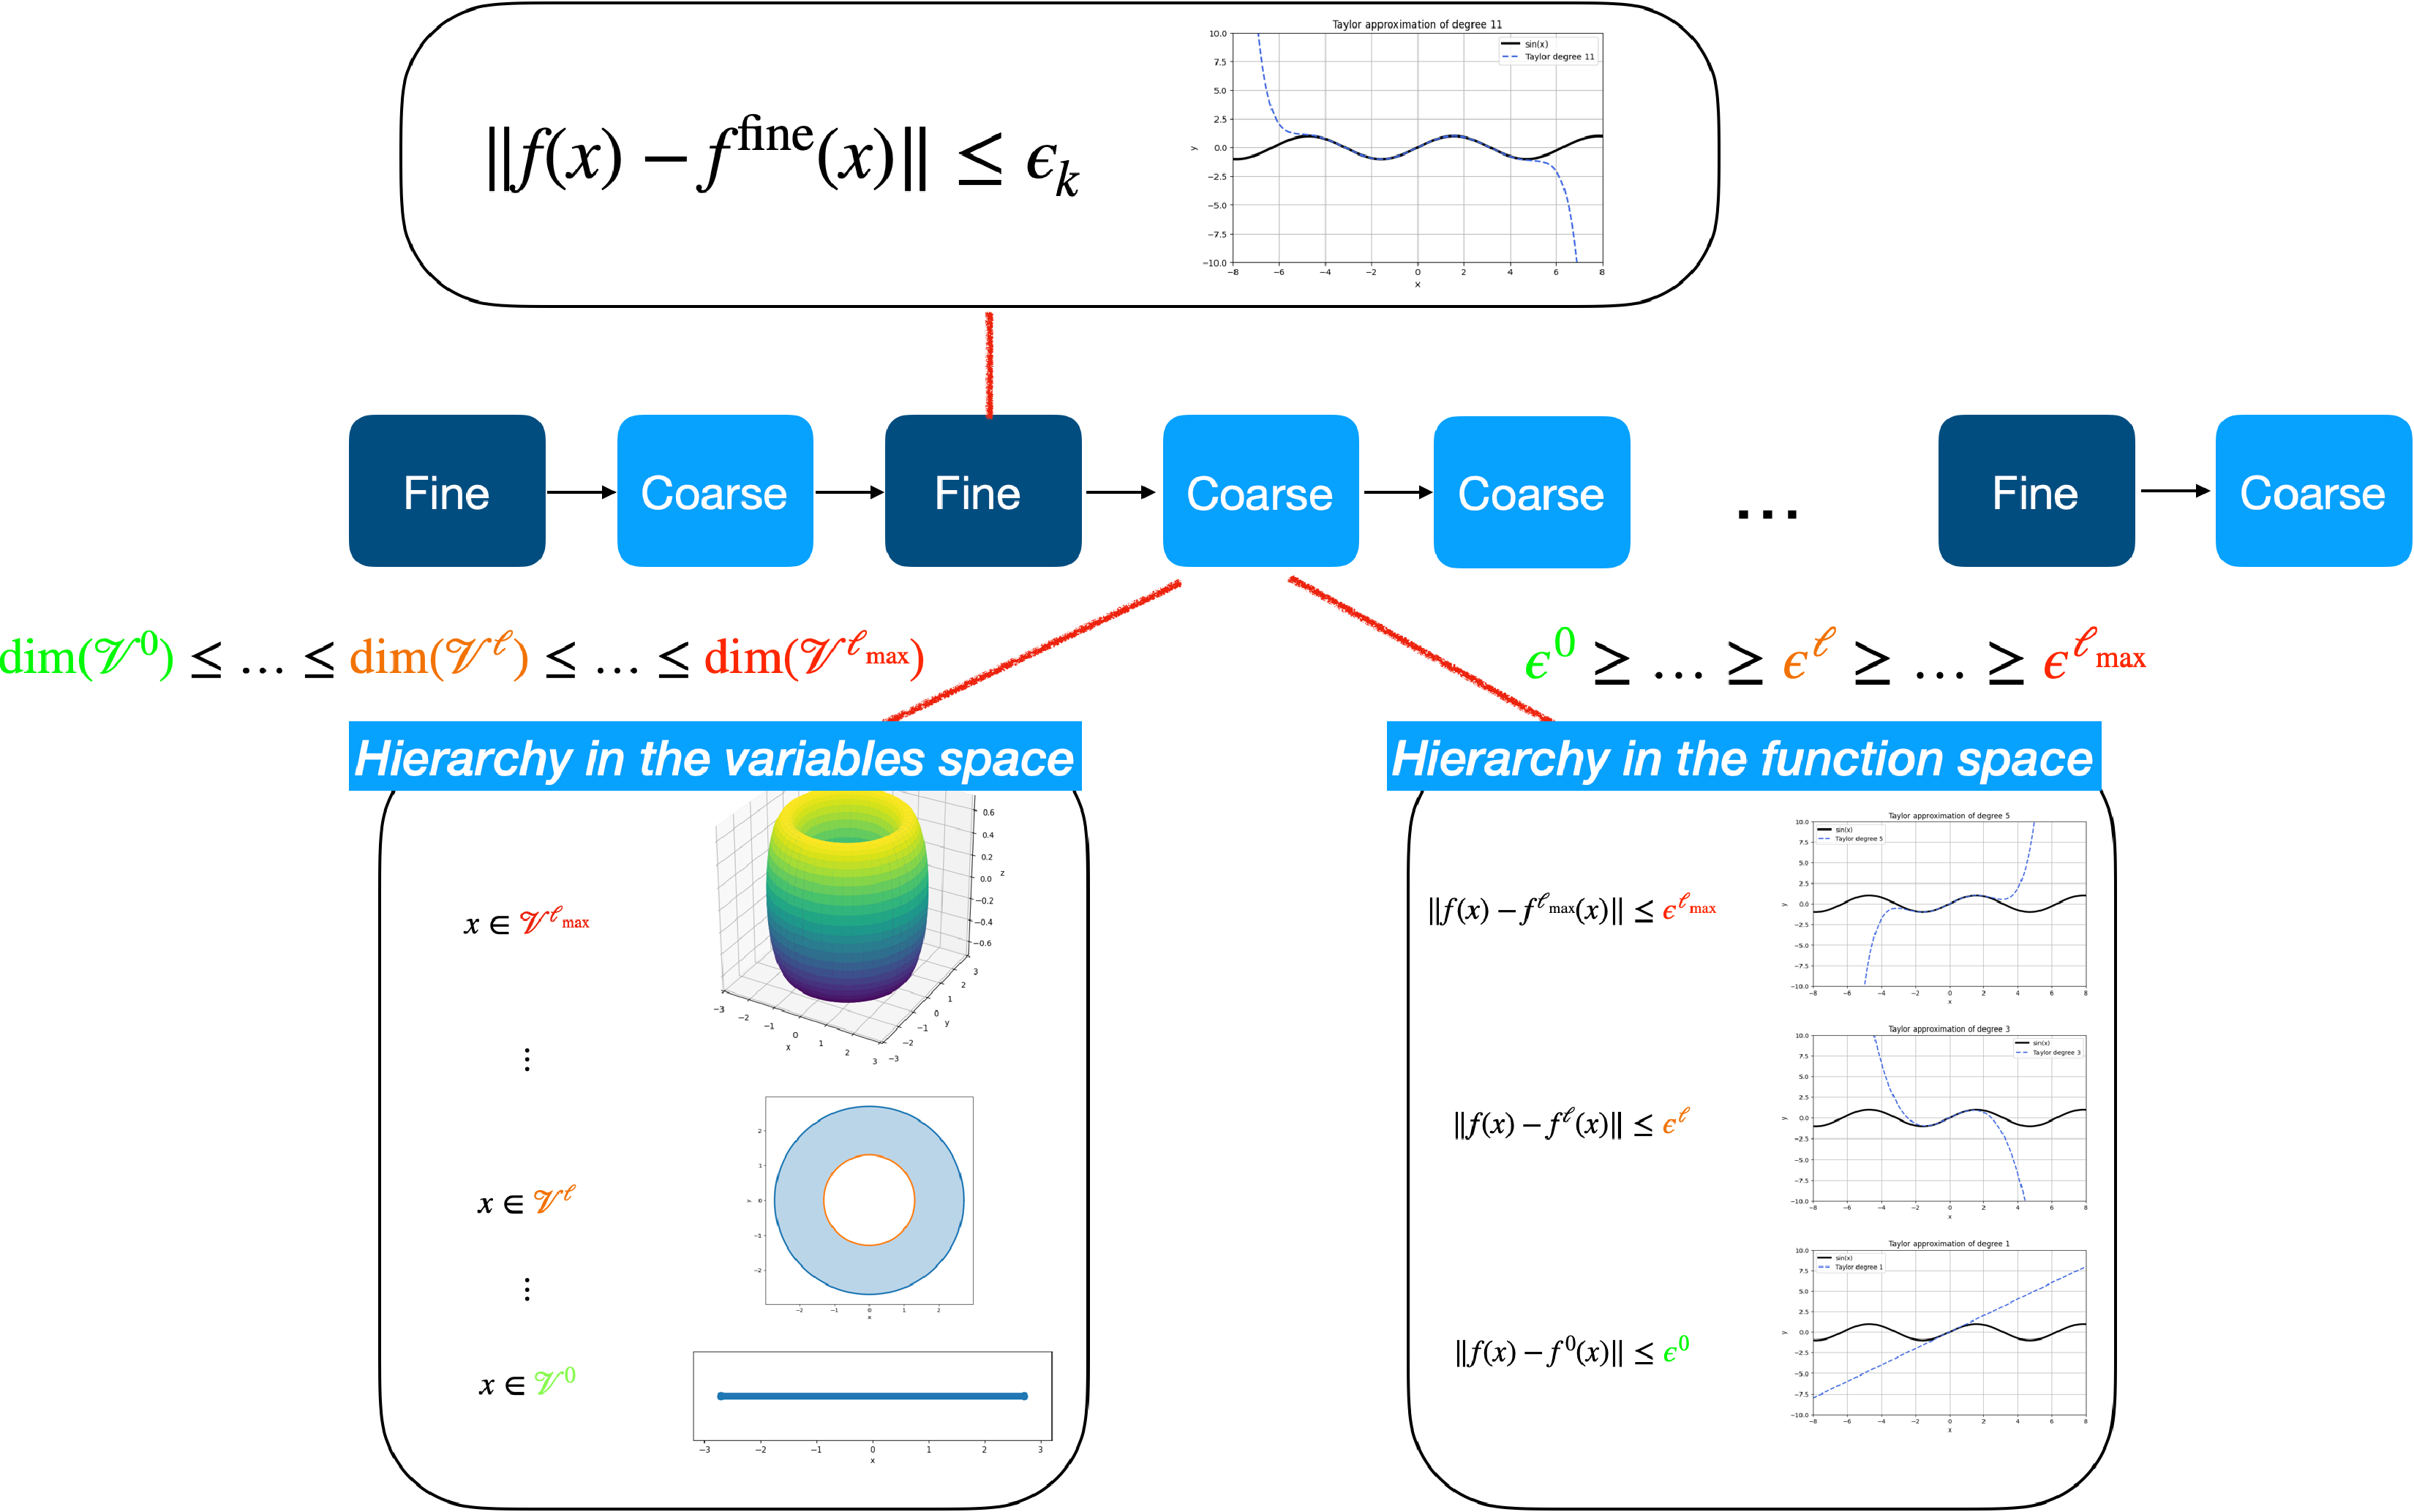
\includegraphics[scale=0.16]{figures/schema_new}
 

% \begin{tiny} \structure{F. Marini, M. Porcelli,  E. Riccietti, 
  % \textbf{A multilevel stochastic regularized first-order method with application to finite sum minimization}, 2026, accepted in Mathematics of computation}  
%\end{tiny}

\vspace{0.5cm}
Convergence with \alert{probability one} for the stochastic process $\{M_k, X_k, S_k, \Lambda_k, F_k\}$. \small{ \textcolor{mygreen}{[  Marini, Porcelli, R., MathComp, 2026]}}


%\begin{footnotesize}
%	\begin{thebibliography}{9}
%		\setbeamertemplate{bibliography item}[article]
%			\bibitem{E} \textit{A multilevel stochastic regularized first-order method with application to finite sum minimization}, {\color{black} F. Marini, M. Porcelli,  E. Riccietti}, {\color{black} 2026}
%				\end{thebibliography} 
%	\end{footnotesize}
	



 \end{frame}


\begin{frame}{My contributions (III) : non-smooth optimization }

$$
\min_x f(x):=\underbrace{L}_{\text{smooth}}(x)+\underbrace{S}_{\text{non-smooth}}(x)
$$
\begin{footnotesize}

\end{footnotesize}
\begin{tcolorbox}[
      title=Forward-backward iterations,
      colback=white,
      colframe=gray!40,
      boxrule=0.4pt,
      arc=4pt,
      left=6pt, right=6pt, top=0pt, bottom=4pt,
    ]
    \vspace{-0.3cm}
\begin{align*}
x_{k+1}&=\operatorname{prox}_{\tau S}(x_k-\tau \nabla L(x_k)),\\
\operatorname{prox}_{\tau S}(x)&:=\arg\min_{y\in\mathbb{R}^n}\left[S(y)+\frac{1}{2\tau}\|y-x\|^2\right]
\end{align*}
 \vspace{-0.3cm}
Multilevel extension: {\small
\textcolor{gray}{%
[P.~Parpas, 2017]}}
%\textbf{A Multilevel Proximal Gradient Algorithm for a Class of Composite
%Optimization Problems}, 2017]}}
\vspace{0.1cm}


\end{tcolorbox}





%\begin{small}
%	\begin{thebibliography}{9}
%		\setbeamertemplate{bibliography item}[article]
%			\bibitem{E} \textit{A Multilevel Proximal Gradient Algorithm for a Class of Composite
%Optimization Problems}, {\color{black} P. Parpas}, {\color{black} 2017}
%				\end{thebibliography} 
%	\end{small}


	\begin{footnotesize}
\begin{tcolorbox}[
        title={ Multilevel inexact inertial proximal method },
    colback=green!10,
    colframe=green!70!black,
        fonttitle=\bfseries,
]
\begin{itemize}
\item Allows for inexact prox evaluations
\item Allows for inertial iterations
\item SOTA convergence guarantees: $\left(f(x_k)-f(x^*)\right)=O\left(\frac{1}{k^2}\right)$\\
\end{itemize}
\end{tcolorbox}
\end{footnotesize}
\footnotesize{ \textcolor{mygreen}{[Lauga, R., Pustelnik, Gonçalves, SIIMS, 2024]}}


\end{frame}

\begin{frame}{My contributions (IV) : multilevel Plug and Play (PnP) }

\centering
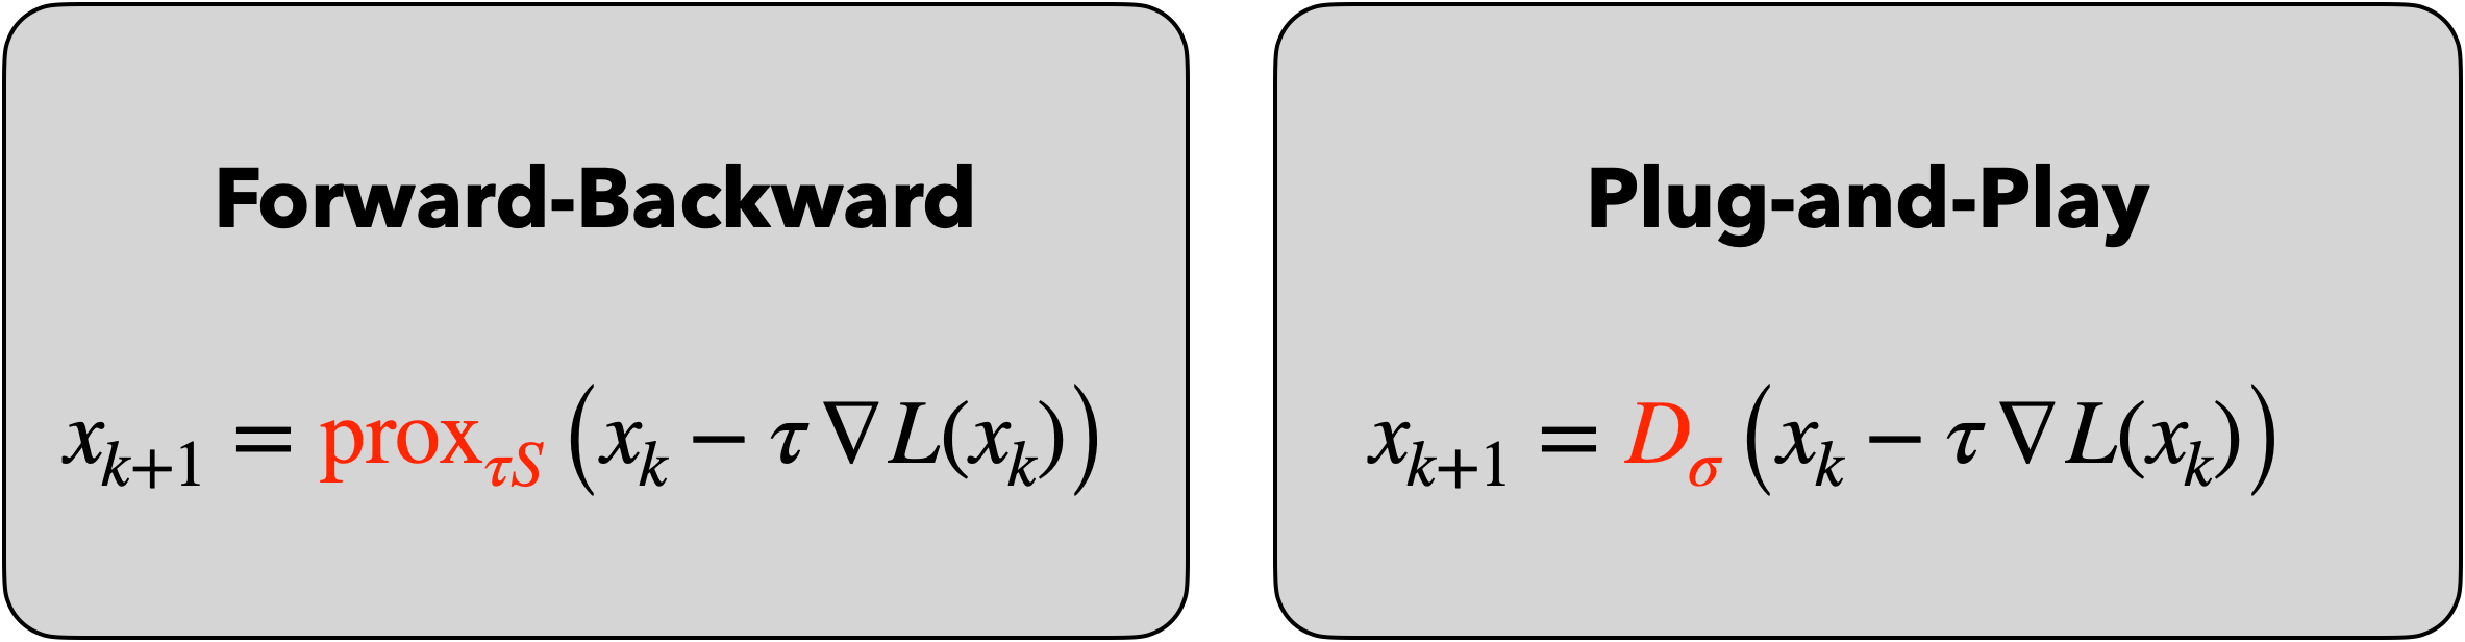
\includegraphics[scale=0.2]{figures/pnp}






%\begin{small}
%	\begin{thebibliography}{9}
%		\setbeamertemplate{bibliography item}[article]
%			\bibitem{E} \textit{A Multilevel Proximal Gradient Algorithm for a Class of Composite
%Optimization Problems}, {\color{black} P. Parpas}, {\color{black} 2017}
%				\end{thebibliography} 
%	\end{small}


	\begin{footnotesize}
\begin{tcolorbox}[
        title={ Multilevel  PnP },
    colback=green!10,
    colframe=green!70!black,
        fonttitle=\bfseries,
]
\begin{itemize}
\item Improves speed and robustness wrt classical PnP
\item First extension of multilevel framework to fixed-point iterations
\end{itemize}
\end{tcolorbox}
\end{footnotesize}

\vspace{0.1cm}
\footnotesize{ \textcolor{mygreen}{[Laurent, Tachella, R., Pustelnik, IEEE TCI, 2025]}}


\end{frame}

\begin{frame}{Still much to do!}
%\begin{itemize}
%\item Extension to generic \alert{fixed-point schemes }
%\item  Convergence of the \alert{iterates}
%\item  \alert{Higher order/preconditioned} non-smooth methods
%\end{itemize}
\includegraphics[width=\textwidth]{figures/perspectives5}

\end{frame}




%\vspace{0.3cm}

%\begin{footnotesize}
%	\begin{thebibliography}{9}
%		\setbeamertemplate{bibliography item}[article]
%			\bibitem{E} \textit{IML FISTA: A Multilevel Framework for Inexact and Inertial Forward-Backward. Application to Image Restoration}, {\color{black} G. Lauga, E. Riccietti, N. Pustelnik, P. Gonçalves}, {\color{black} 2024}
%				\end{thebibliography} 
%	\end{footnotesize}





\begin{comment}
\begin{frame}{Coarse model for the non-smooth case: smoothing }
\begin{columns}
\begin{column}{0.48\textwidth}
$
F_k^H(s^H)=\overbrace{f^H(x^H_{k,0}+s^H)}^{\text{non-smooth}}+\langle s^H, v_k^H\rangle
$

 $v_k^{H}=R\alert{\nabla f^h}(x_k^{h})-\alert{\nabla f^{H}} (x_{k,0}^{H})$
\end{column}
\begin{column}{0.48\textwidth}
\alert{Smoothing technique}: \\$g$ non-smooth $\rightarrow$ $g_\gamma$ smooth
 \end{column}
    \end{columns}
    
    
    
\begin{columns}
\begin{column}{0.48\textwidth}

{Example: the Moreau envelope}
 $\mbox{\textcolor{cyan}{$\leftidx{^{\gamma}}{g}$}} = \inf_{y \in \mathcal{\footnotesize{H}}}g(y) + \frac{1}{2 \gamma} \Vert \cdot -y \Vert^2$
\end{column}
\begin{column}{0.48\textwidth}

 \begin{tcolorbox}[
      title=Moreau envelope of \textcolor{cyan}{$\ell_1$}-norm for \textcolor{orange}{$\gamma = 0.1$} and \textcolor{yellow}{$\gamma = 1$}
,
      colback=white,
      colframe=gray!40,
      boxrule=0.4pt,
      arc=4pt,
      left=6pt, right=6pt, top=4pt, bottom=4pt,
    ]
\begin{figure}
    \includegraphics[width = 0.3\textwidth]{images/moreauL1.eps}
    \end{figure}
    \end{tcolorbox}
    \end{column}
    \end{columns}
    
     \begin{tcolorbox}[
      title=Coarse models,
      colback=white,
      colframe=gray!40,
      boxrule=0.4pt,
      arc=4pt,
      left=6pt, right=6pt, top=4pt, bottom=4pt,
    ]

  %  \begin{itemize}
    %\item $
 %F_k^{H}(s^H) = \Lo^H(Ry_k^h+s^H) + \alert{{S^H_{\gamma_H}}} (Ry_k^h+s^H) + (\textcolor{myblue}{v_k^H})^Ts^H$
 %\item 
%$F_k^{H} (s^H) = \Lo^H (Ry_k^h+s^H) + \alert{S^{H}} (Ry_k^h+s^H) +  (\textcolor{myblue}{v_k^H})^Ts^H$
%\end{itemize}
  \begin{itemize}
    \item $
 F_k^{H}= \Lo^H + \alert{{S^H_{\gamma_H}}} + \langle\textcolor{myblue}{v_k^H},s^H\rangle$ (smooth)
% \item 
%$F_k^{H}  = \Lo^H  + \alert{S^{H}} +  \langle\textcolor{myblue}{v_k^H},s^H\rangle$ (non-smooth)
\end{itemize}
$\textcolor{myblue}{v_k^H}= R  \left(\nabla \Lo^h(y_k^h) + \alert{\nabla S^h_{\gamma_h}}(y_k^h)\right) -(\nabla \Lo^H(R  y_k^h) + \alert{\nabla S^H_{\gamma_H}}(R  y_k^h))$
\end{tcolorbox}
\end{frame}

\end{comment}













\part{Exploiting hierarchies in imaging problems}
\frame[plain]{\partpage}

\begin{frame}{Image reconstruction problems }
\begin{columns}
\begin{column}{0.3\textwidth}
\begin{tcolorbox}[
      title=Direct problem,
      colback=white,
      colframe=gray!40,
      boxrule=0.4pt,
      arc=4pt,
      left=6pt, right=6pt, top=2pt, bottom=4pt,
    ]
    \vspace{-0.3cm}
$$
z=A\bar x+ \epsilon
$$
\end{tcolorbox}
\end{column}
\begin{column}{0.68\textwidth}
\begin{tcolorbox}[
      title=Inverse problem,
      colback=white,
      colframe=gray!40,
      boxrule=0.4pt,
      arc=4pt,
      left=6pt, right=6pt, top=4pt, bottom=4pt,
    ]

$$
\widehat{x} \in\underset{x}{\arg\min}\; \underbrace{\frac{1}{2}\Vert A x - z \Vert_2^2}_{L} + \underbrace{\lambda \Vert D x\Vert}_{S}
$$
\end{tcolorbox}
\end{column}
\end{columns}

%with $ \Vert L x \Vert_\star$ usually sparsity inducing norm.

%\begin{minipage}{0.6\textwidth}
\begin{table}
\begin{tabular}{ccc}
\includegraphics[trim={0.1em 0.1em 0.1em 0.1em},clip,width=0.25\textwidth]{images/slide1/x_originale-crop.pdf} &
\includegraphics[trim={0.1em 0.1em 0.1em 0.1em},clip,width=0.25\textwidth]{images/slide1/z_degraded-crop.pdf}& 
\includegraphics[trim={0.1em 0.1em 0.1em 0.1em},clip,width=0.25\textwidth]{images/slide1/x_reconstruiteNLTV-crop.pdf} \\
$\overline{x}$ & z&  $\widehat{x}$
\end{tabular}
\end{table}
%\end{minipage}

How to define a hierarchy? 
\begin{itemize}
\item Hyperspectral imaging
\item Radio-interferometry
\end{itemize}


\end{frame}

\begin{comment}

 \begin{frame}{Example 1: image restoration}





\begin{columns}
\begin{column}{0.5\textwidth}
\hspace{1cm}
\centering
\includegraphics[scale=0.12]{images/vitt_vert}
\end{column}

\hspace{1cm}
\vspace{-10cm}
\begin{column}{0.5\textwidth}
\centering
\includegraphics[scale=0.2]{images/wavelets}
\end{column}
\end{columns}


\end{frame}

\begin{frame}{Example 2: hyperspectral imaging }
%\mbox{} \\
%\mbox{} \\
\centering
%\includegraphics[trim={1em 0.2em 1em 0.1em},clip,width = 1\textwidth]{images/TransfertInfoIHS.pdf}
    \includegraphics[width=0.9\textwidth]{TransfertInfoHYSpatial-crop.pdf}
        \includegraphics[width=1\textwidth]{TransfertInfoHYSpectral-crop.pdf}
\end{frame}
\end{comment}


\begin{frame}{1) Hyperspectral imaging}


\begin{columns}
\begin{column}{0.68\textwidth}
\begin{center}
    \includegraphics[width = 0.6\textwidth]{images/Hypercube-crop.png}
\end{center}
\end{column}
\begin{column}{0.3\textwidth}
\begin{itemize}
\item Deblurring 
\item Inpainting 
\end{itemize}

\end{column}
\end{columns}


\begin{tcolorbox}[
      title=Fine level,
      colback=white,
      colframe=gray!40,
      boxrule=0.4pt,
      arc=4pt,
      left=6pt, right=6pt, top=4pt, bottom=4pt,
    ]

$$
f(x)= \underbrace{\frac{1}{2}\Vert \alert{A} x - z \Vert_2^2}_{L} + \underbrace{\lambda \sum_i\| (\alert{D} x)(i)\|_\star}_{S}
$$

\end{tcolorbox}
%\end{column}
%\begin{column}{0.68\textwidth}
\begin{tcolorbox}[
      title=Coarse approximation,
      colback=white,
      colframe=gray!40,
      boxrule=0.4pt,
      arc=4pt,
      left=6pt, right=6pt, top=4pt, bottom=4pt,
    ]

$$
f^H(x^H):=\underbrace{\frac{1}{2}\Vert \alert{A^H} x^H - \textcolor{myblue}{R} z \Vert_2^2}_{L^H} + \underbrace{\lambda \sum_i\| (\alert{D^H} x)(i)\|_\star}_{S^H}
$$
\end{tcolorbox}
%\end{column}
%\end{columns}
  %  \begin{equation*}
    %\widehat{x} \in \underset{x\in \mathbb{R}^N}{\textrm{Argmin}} \frac{1}{2} \Vert A x-\mathrm{z} \Vert_2^2 + \lambda g (\D x) 
      % \end{equation*}
       %$A \in \mathbb{R}^{M \times N}$: inpainting operator 
      %\begin{equation*}
         %   (\forall x\in \mathbb{R}^{N}) \quad  g(\D x) = \sum_{i=1}^{N} \Vert (\D x)^i \Vert_{*}
        %\end{equation*}

\end{frame}
\begin{frame}{How to build the hierarchy?}
\mbox{} \\
\mbox{} \\
\centering
%\includegraphics[trim={1em 0.2em 1em 0.1em},clip,width = 1\textwidth]{images/TransfertInfoIHS.pdf}
\only<1>{\includegraphics[width = 1\textwidth]{images/TransfertInfoHYSpatial-crop.pdf}}
\pause
\only<2>{\includegraphics[width = 1\textwidth]{images/TransfertInfoHYSpectral-crop.pdf}}
\end{frame}
\begin{comment}
\begin{frame}{Coarse model construction}

    \begin{columns}[t]
      \begin{column}{0.5\textwidth}
      \begin{center}Spectral IML FISTA\end{center}
      \footnotesize
        \begin{algorithm}[H] 
        $b,\ell = 1$ \\
          \While{$b\leq L_h-1$}{
          \eIf{\small $\mu(\lambda) - \sigma(\lambda) \leq \lambda^{(b+1)}-\lambda^{(b)}\leq \mu(\lambda) + \sigma(\lambda)$}{
            $x_H^{(:,\ell)} = \frac{1}{2}(x_h^{(:,b)}+x_h^{(:,b+1)})$, \\$\ell = \ell +1$
            }{
             $x_H^{(:,\ell)} = x_h^{(:,b)}$, \\$x_H^{(:,\ell+1)} = x_h^{(:,b+1)}$, \\$\ell = \ell +2$
             }
           $b = b+2$ 
          }
  %\caption{Agrégation des bandes}
  \label{alg:fusion}
\end{algorithm}
The blocks of $A_h$ are passed through this procedure to construct the blocks of $A_H$.
      \end{column}
      \begin{column}{0.5\textwidth}
      
      \begin{center}Spatial IML FISTA\end{center}
      \footnotesize
        \begin{align*}
    (\forall & b=\{1,\ldots,L_h\}) \\ & x_H^{(:,b)} = I_H^h(x_h^{(:,b)})
\end{align*}
where:
\begin{equation*}
\begin{split}
I_H^h & :=\left( \mathbf{R}_{\mathbf{q},r} \otimes \mathbf{R}_{\mathbf{q},c} \right) 
\end{split}
\end{equation*}
$T^{\text{dec}}_{N_{H,c}}(\mathbf{q})$ decimated Toeplitz matrix engendered by $\mathbf{q}$.

The blocks of $A_h$ are decimated to construct the blocks of $A_H$.
      \end{column}
\end{columns}
\end{frame}
\end{comment}

%\begin{frame}{}


% \includegraphics[trim={0.1em 0.1em 0.1em 0.1em},clip,width=0.45\textwidth]{images//X-crop.pdf} 
%\includegraphics[trim={0.1em 0.1em 0.1em 0.1em},clip,width=0.45\textwidth]{images//ZChris-crop.pdf} \\
%$\bar{x} \in \mathbb{R}^{512 \times 512 \times 33}$ 
%$z$
%\\
 %\includegraphics[trim={0.1em 0.1em 0.1em 0.1em},clip,width=0.65\textwidth]{images//FISTA50SpecChris-crop.pdf} 
%\includegraphics[trim={0.1em 0.1em 0.1em 0.1em},clip,width=0.65\textwidth]{images//IMLFISTA50SpecChris-crop.pdf} \\
%$x_{\text{end,FISTA}}$ 
%$x_{\text{end,IML FISTA}}$
%\end{frame}
{
\setbeamercolor{background canvas}{bg=white}
\begin{frame}{Objective function evolution}
  %  \includegraphics[trim={3em 2.5em 0 0},clip,width=1\textwidth]{images//FHCPU_IChris_L1nuclearNLTV_0.01_EN-crop.pdf}
  \centering
\includegraphics[width=\textwidth]{figures/hyper_f3}

%\begin{footnotesize}
%	\begin{thebibliography}{9}
%		\setbeamertemplate{bibliography item}[article]
%			\bibitem{E} \textit{Méthodes multi-niveaux pour la restauration d'images hyperspectrales}, {\color{black} G. Lauga, E. Riccietti, N. Pustelnik, P. Gonçalves}, {\color{black} 2023}
%				\end{thebibliography} 
%	\end{footnotesize}



\end{frame}
}
%\begin{frame}{Results with Spectral IML FISTA}
   % \centering
    %\begin{tabular}{ccc}
     %$\bar{x}$ (SNR) & $x_{2,\text{FISTA}}$ (7 dB) & $x_{\text{end,FISTA}}$ (21 dB)\\
     %\includegraphics[trim={0.1em 0.1em 0.1em 0.1em},clip,width=0.3\textwidth]{images/slide_HY/X-crop.pdf}    & \includegraphics[trim={0.1em 0.1em 0.1em 0.1em},clip,width=0.3\textwidth]{images/slide_HY/FISTA2SpecChris-crop.pdf} & \includegraphics[trim={0.1em 0.1em 0.1em 0.1em},clip,width=0.3\textwidth]{images/slide_HY/FISTA50SpecChris-crop.pdf} \\
     %\includegraphics[trim={0.1em 0.1em 0.1em 0.1em},clip,width=0.3\textwidth]{images/slide_HY/ZChris-crop.pdf}    & \includegraphics[trim={0.1em 0.1em 0.1em 0.1em},clip,width=0.3\textwidth]{images/slide_HY/IMLFISTA2SpecChris-crop.pdf} & \includegraphics[trim={0.1em 0.1em 0.1em 0.1em},clip,width=0.3\textwidth]{images/slide_HY/IMLFISTA50SpecChris-crop.pdf} \\
     %$\mathrm{z}$ (3 dB) & $\mathrm{x}_{2,\text{IML FISTA}}$ (19 dB)& $\mathrm{x}_{\text{end,IML FISTA}}$ (35 dB)\\
    %\end{tabular}

%\end{frame}

\begin{frame}{Reconstruction}
\centering
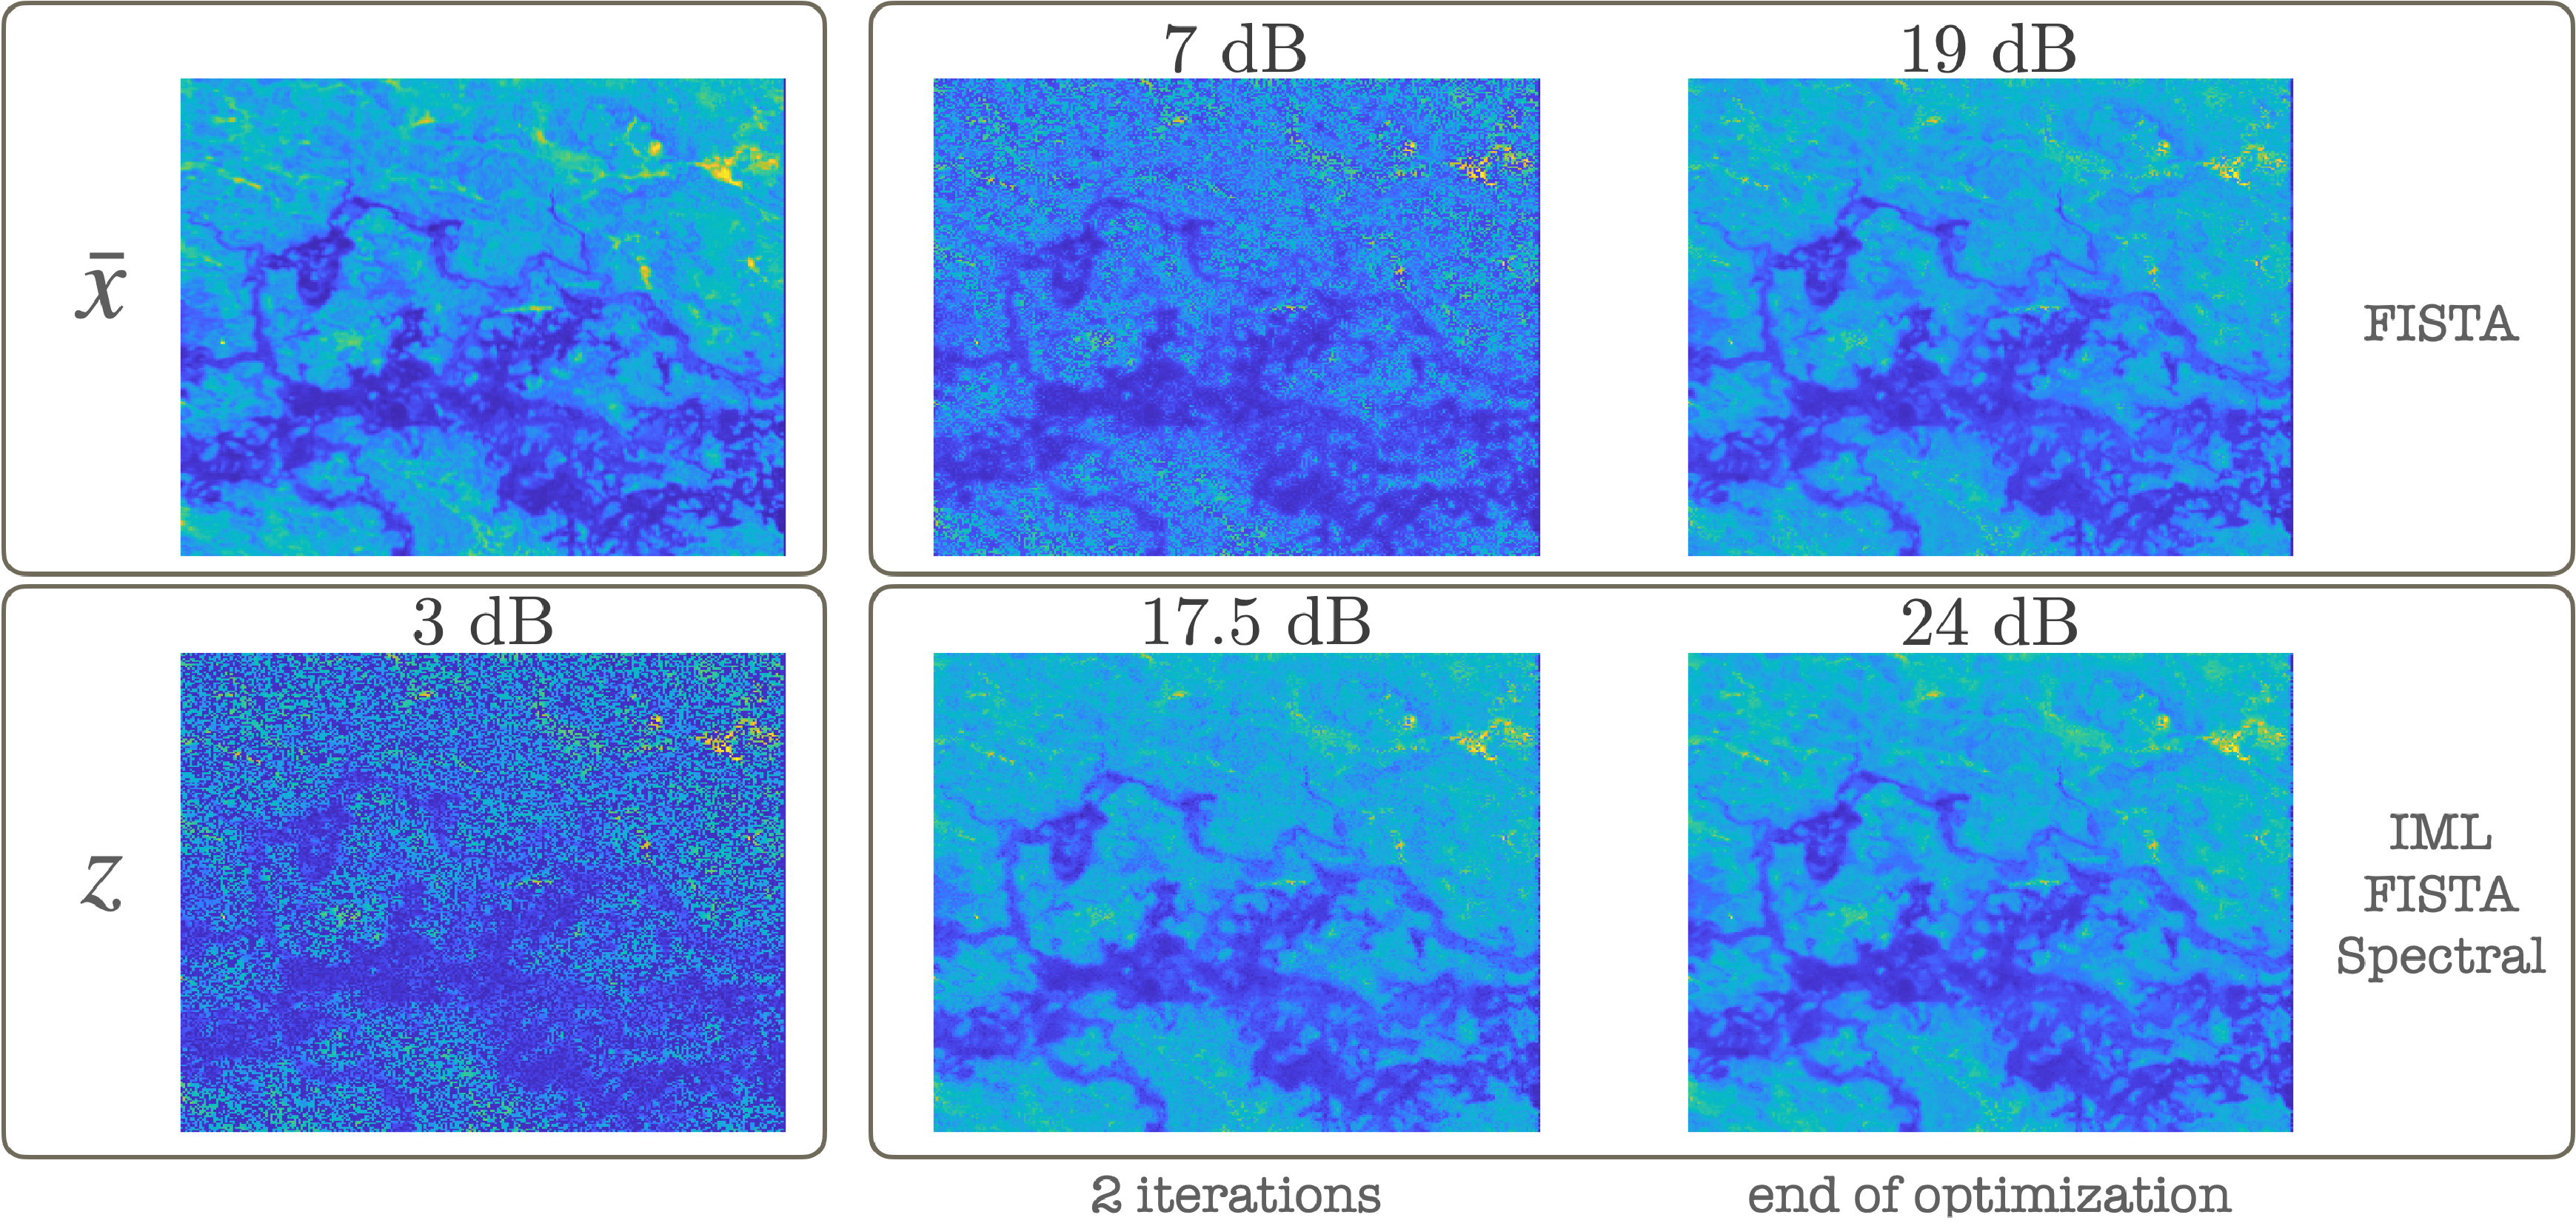
\includegraphics[width=\textwidth]{figures/hyper_image}
$$
\text{PSNR} \bm{\uparrow}
$$
\vspace{0.5cm}

        \small{ \textcolor{mygreen}{[Lauga, R., Pustelnik, Gonçalves, GRETSI, 2023]}}

\end{frame}

%\subsection{Radio-interferometric imaging}


\begin{frame}{2) Radio-interferometric imaging}
\centering
\includegraphics[width=\textwidth, trim=0 2cm 0 0, clip]{RI}
$$
 f_i(x)=\frac{1}{2}\|A x-z\|^2+\|W_iD^*x\|_1+i_{\mathbb{R}^n_+}(x), \quad x\in\mathbb{R}^n
$$


\alert{Dimension bottleneck: number of observations}
$$
 f_i^H(x)=\frac{1}{2}\|\alert{R}(A x-z)\|^2, \quad x\in\mathbb{R}^n
$$
\end{frame}

\begin{frame}{Building the hierarchy}
\centering
\includegraphics[width=\textwidth]{RI2}

\end{frame}
%\begin{frame}{Building the hierarchy}
%\centering
%\includegraphics[width=\textwidth]{RI3}
%\begin{footnotesize}
%	\begin{thebibliography}{9}
%		\setbeamertemplate{bibliography item}[article]
%			\bibitem{E} \textit{A multilevel framework for accelerating uSARA in radio-interferometric imaging}, {\color{black} G. Lauga, A. Repetti, E. Riccietti, N. Pustelnik, P. Gonçalves, Y. Wiaux}, {\color{black} 2024}
%				\end{thebibliography} 
%	\end{footnotesize}

%\small{ \textcolor{mygreen}{[G. Lauga, A. Repetti, E. Riccietti, N. Pustelnik, P. Gonçalves, Y. Wiaux, EUSIPCO, 2024]}}
%\end{frame}


\begin{frame}{Numerical results: objective function}
\centering
\includegraphics[width=\textwidth]{figures/RI_f}%RI6


\end{frame}

\begin{frame}{Numerical results: reconstruction }
\centering
\includegraphics[width=1.05\textwidth]{RI5}
$$
\text{PSNR (dB)} \bm{\uparrow}
$$

\vspace{0.5cm}
\scriptsize{ \textcolor{mygreen}{[Lauga, Repetti, R., Pustelnik, Gonçalves,  Wiaux, EUSIPCO, 2024]}}


\end{frame}











	\part{Exploiting hierarchies in learning problems }
	\frame[plain]{\partpage}
	
	\begin{frame}{Special structure of learning problems}
	Given a dataset $\{(z_i,y_i)\}_{i=1}^m$
	\begin{align*}%\label{eq_sum}
\min_{\theta\in\R^{\alert{n}}} f_{z,y}(\theta)&=\sum_{i=1}^{\alert{m}} f_{z_i,y_i}(\theta), \quad \theta=(W_1,b_1,\dots,W_L,b_L) \\ 
f_{z_i,y_i}(\theta)&:= L(\sigma\circ(W_L z_i -b_L)\circ\dots\circ\sigma\circ(W_1 z_i-b_1)-y_i),
\end{align*}
%for a set of data $\{(x_i,y_i)\}_{i=1}^m$ and a loss function $\mathcal{L}$.

\centering
%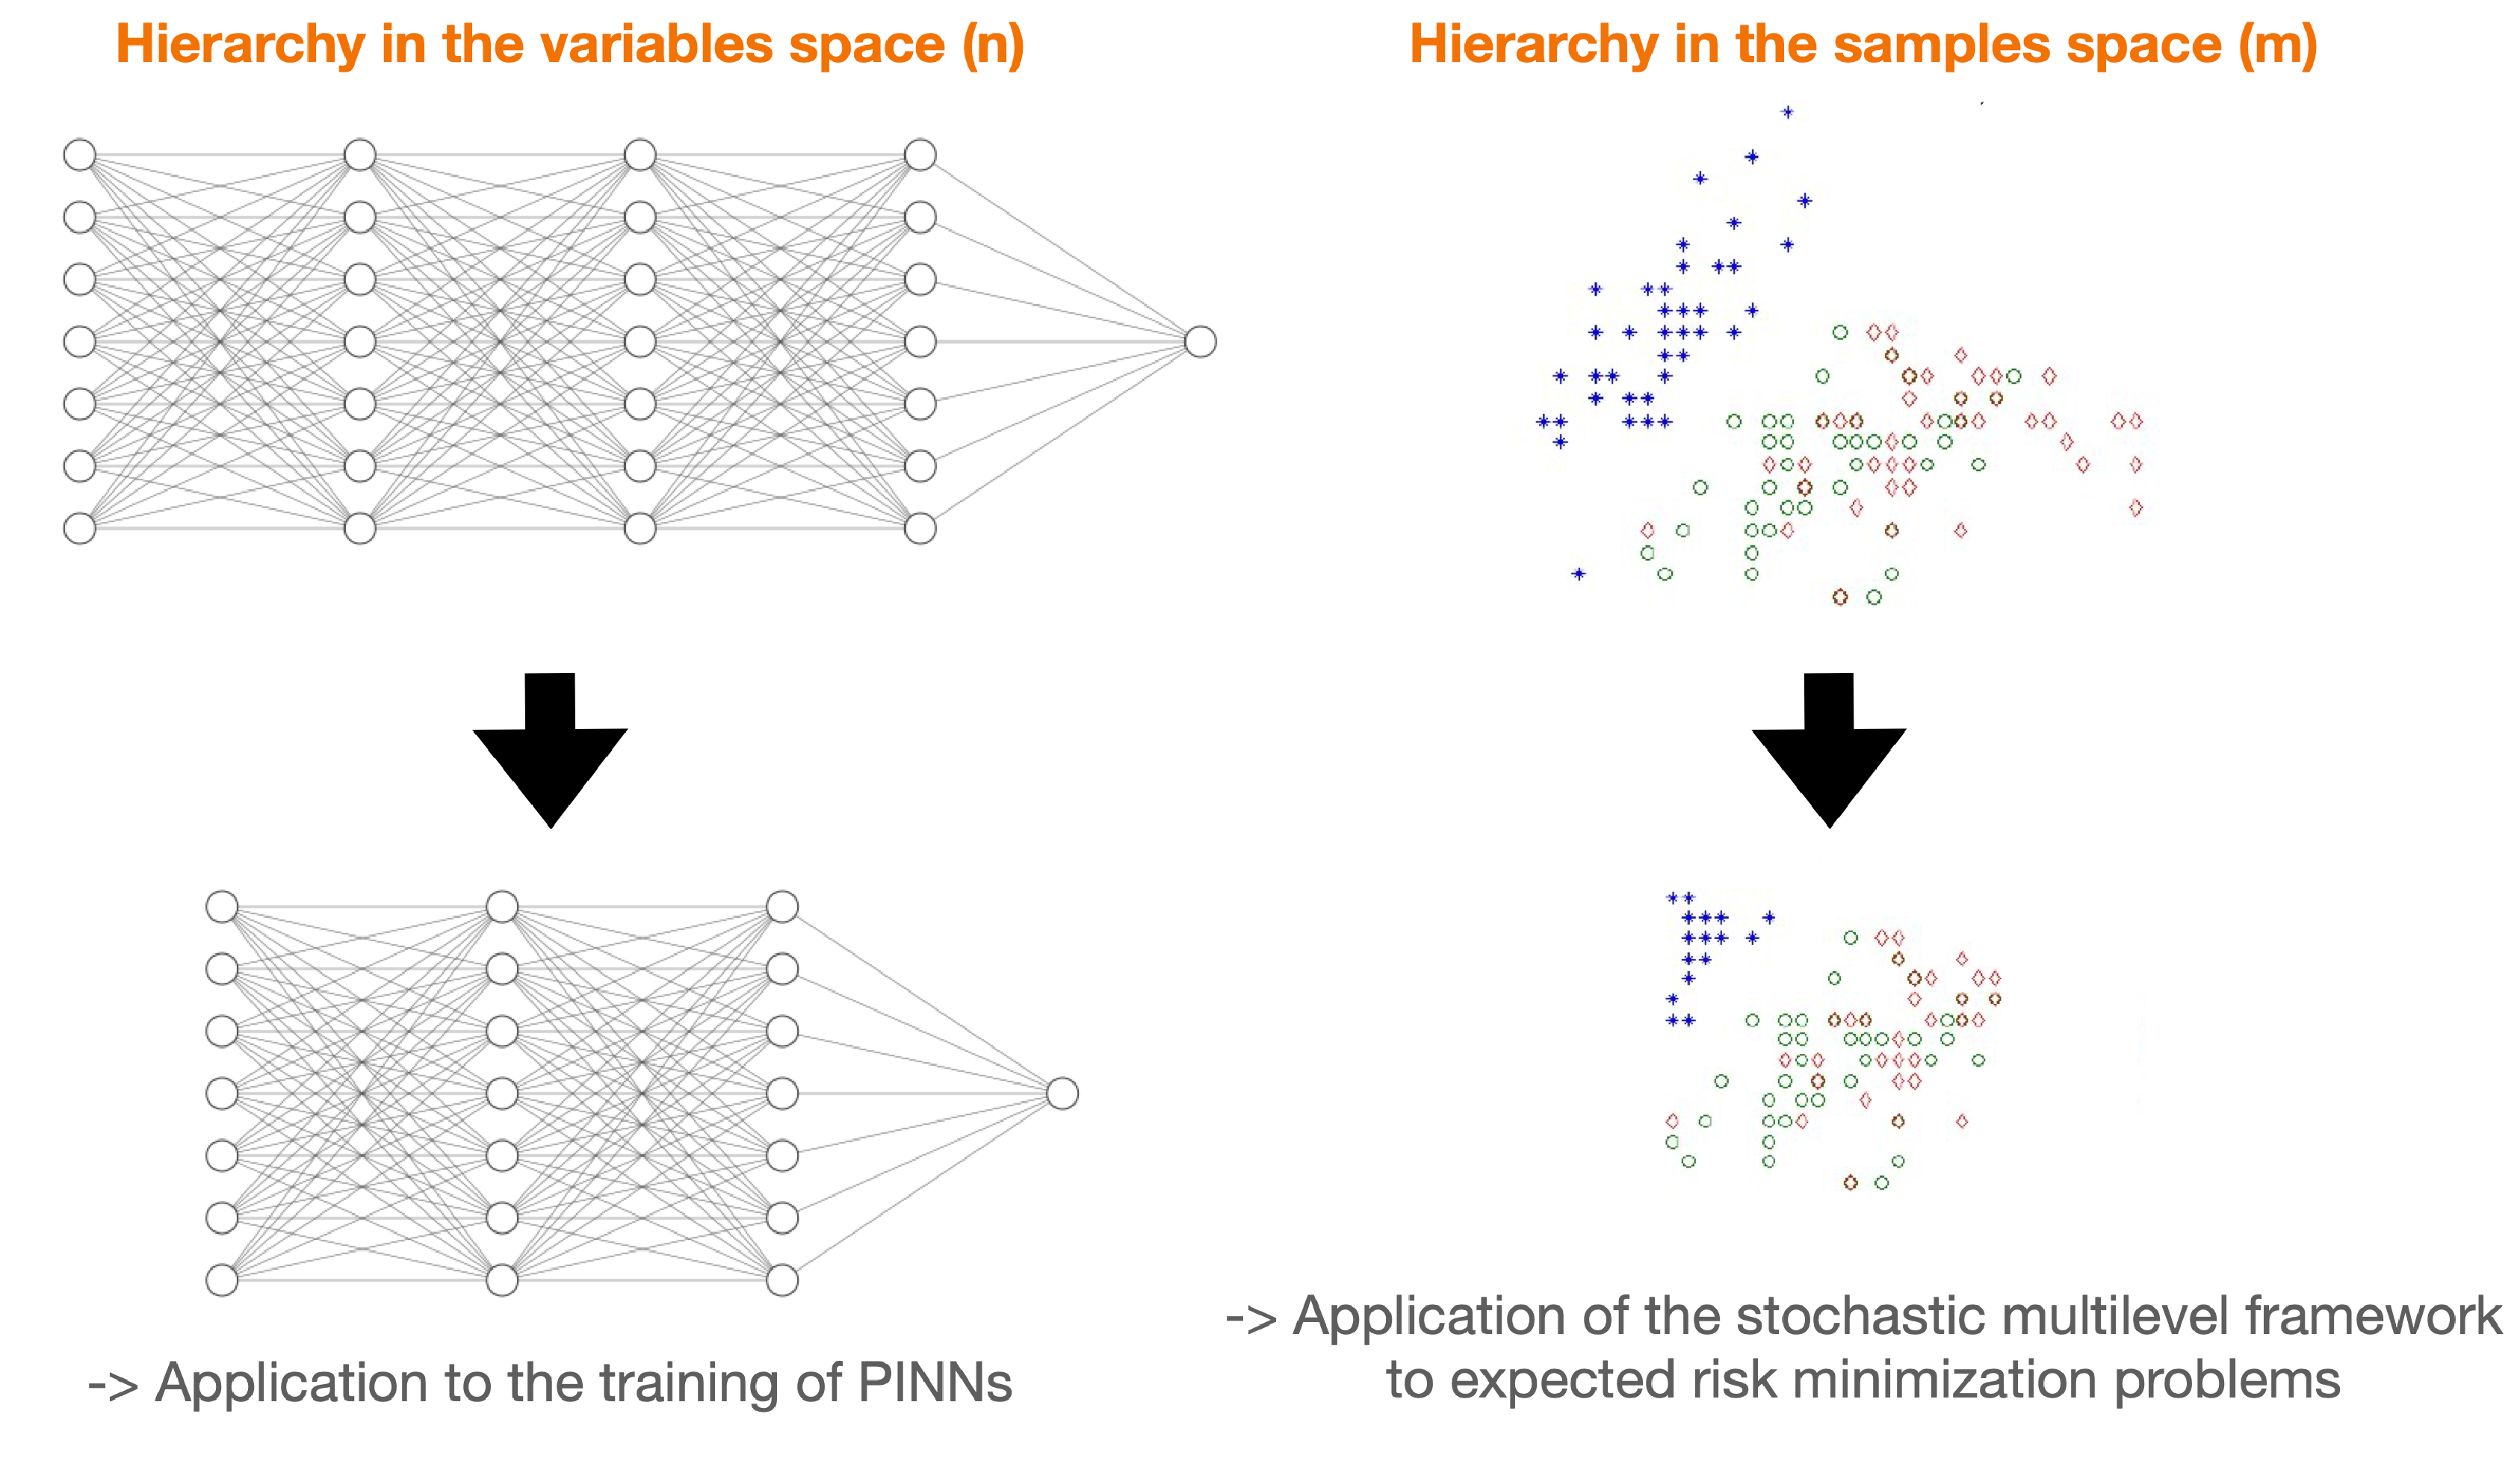
\includegraphics[scale=0.15]{figures/proj_learning3}
%\includegraphics[scale=0.15]{figures/learning_hierarchy}
\includegraphics[scale=0.15]{figures/learning_hierarchy2}


	
	\end{frame}
	
	

 






	
	\begin{frame}{Physics informed neural networks (PINNs) training}
	
	\vspace{-0.5cm}

				\begin{align*}
				\mathcal{L}u(z)=\phi(z) \; in\;\Omega &&
				\mathcal{B}u(z)=\psi(z)\; in\;\partial\Omega
				\end{align*}
				
				

\begin{table}
\begin{tabular}{lc}
Find $\theta$ such that  $ u_{\theta}(z)\approx u(z)$ for all $z\in\Omega$ & Training data\\

    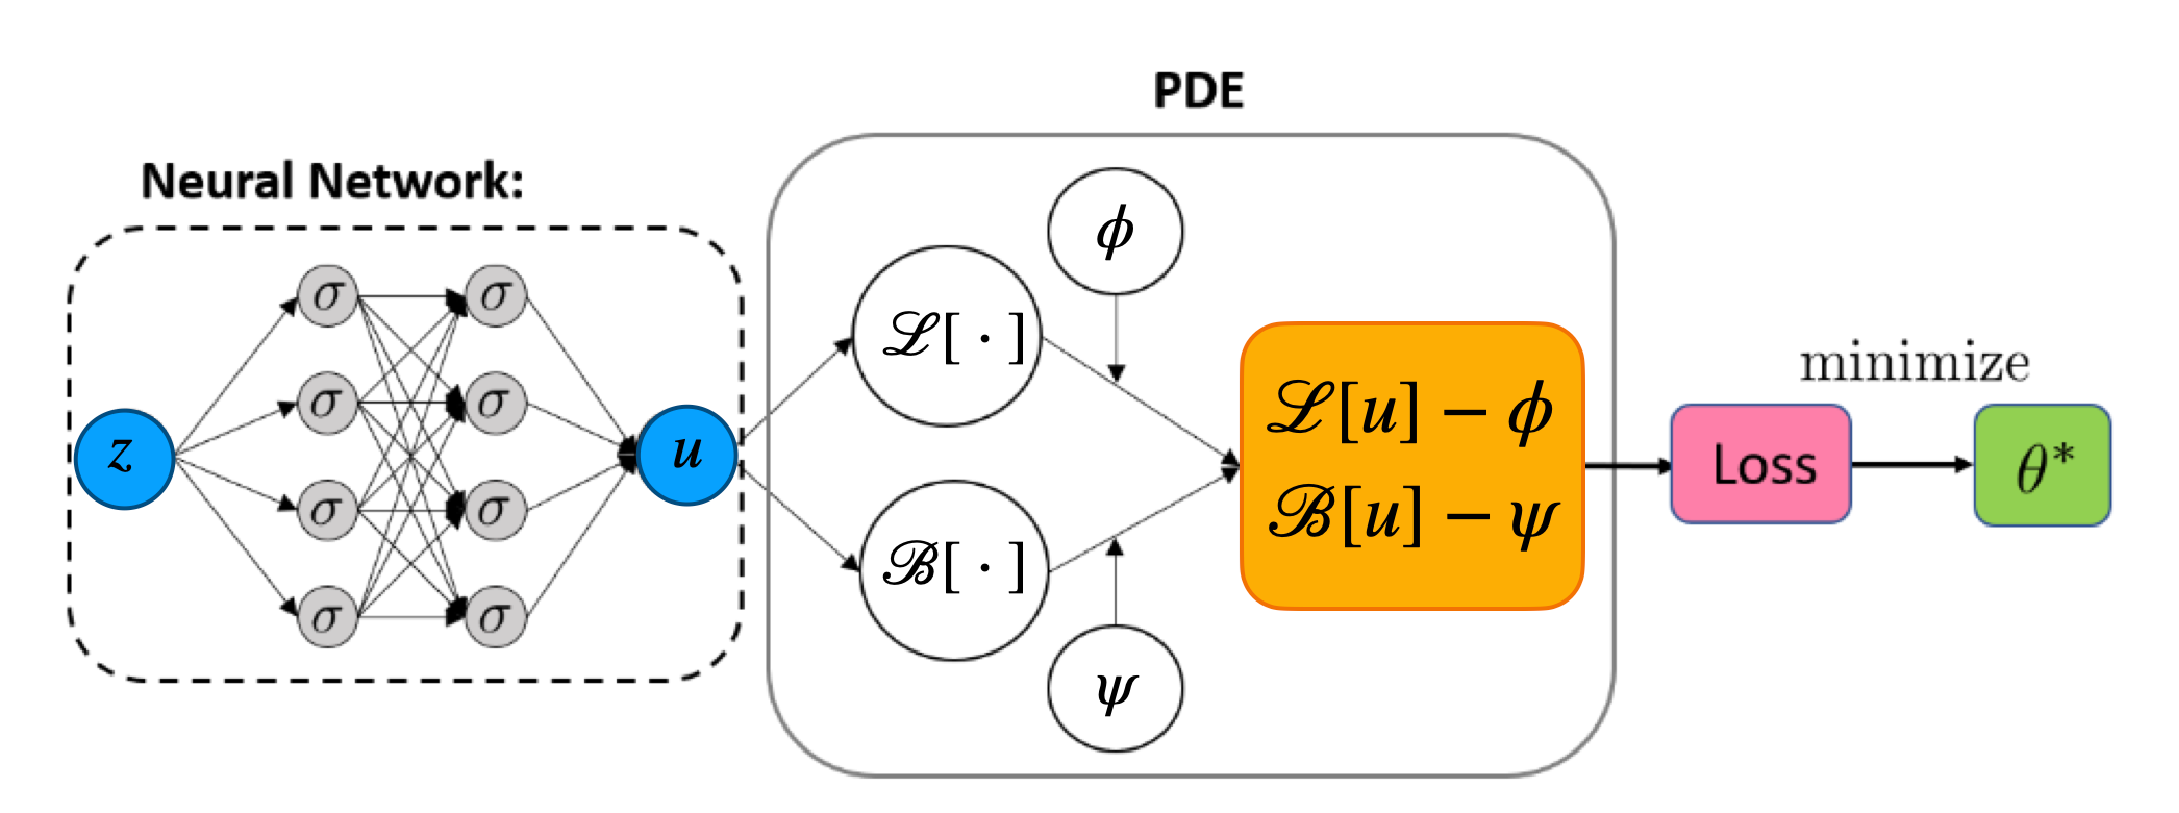
\includegraphics[scale=0.18]{figures/pinn_schema2}&
   
    \includegraphics[scale=0.15]{images/sampling2.png}
   \end{tabular}
\end{table}



%\vspace{0.5cm}

Training problem:
$\displaystyle{\min_\theta  f_{z,y}(\theta)={ \color{red} L_{OBS}(\theta)}+{ \color{orange}L_{PDE}(\theta)}+\color{blue}L_{BC}(\theta)}$
   
\begin{footnotesize}
\begin{align*}
 { \color{red} L_{OBS}(\theta)} & {\small =\gamma_1\sum_{z_i\in\Omega \cup  \partial \Omega} (u_{\theta}(z_i)-y_i)^2},  \\ 
  {\color{orange} L_{PDE}(\theta)}&{\small=\gamma_{2}\sum_{z_i\in \Omega}(\mathcal{L}(u_{\theta}(z_i))-\phi(z_i))^2}
  \\
  {\color{blue} L_{BC}(\theta)}&{\small =\gamma_{3} \sum_{z_i\in \partial\Omega}(\mathcal{B}(u_{\theta}(z_i))-\psi(z_i))^2}
\end{align*}
   \end{footnotesize}

			\begin{tiny}
				\textcolor{gray}{[M. Raissi, P. Perdikaris, G. Karniadakis,  2019]}
				\end{tiny}
				\end{frame}

	
	
	

\begin{frame}{Spectral bias: link with multigrid theory}
%Eigenvalue spectrum decays rapidly as a function of
%frequency:
\begin{itemize}

\item Neural networks:    \alert{high-frequency} components limits  overall speed of learning \begin{tiny}
				\textcolor{gray}{[N. Rahaman, et all., 2019]}
				\end{tiny}



				


				

\begin{figure}
\includegraphics[width=\textwidth]{figures/spectral_bias}
%  \caption{
   % The network prediction $u_{\theta}$ (purple) is reported at training iterations 100 (left), 1500 (middle), and 7500 (right).}
    %\label{fig:spectral_bias}
\end{figure}



 \item Fixed point schemes: hard to reduce the \alert{low frequency} components of the error \begin{tiny}
				\textcolor{gray}{[W. Briggs, V. Henson, S. McCormick, 2000]}
				\end{tiny}



 
   

\begin{figure}
    \centering
  %  \includegraphics[width=0.45\linewidth]{images/waves.png}
    %\includegraphics[width=0.45\linewidth]{images/error_decrease.png}
      \includegraphics[width=0.8\linewidth]{images/MG_new_color.pdf}
  \end{figure}
  \end{itemize}
  \end{frame}


\begin{comment}
\begin{frame}{How to make the methods efficient on all frequencies?}

\centering
\vspace{0.5cm}
\alert{Frequency shift! }
\includegraphics[width=0.8\textwidth]{images/grids}
\vspace{0.5cm}
\begin{itemize}
    \item {\bf Fine} grid $\Omega^h$ with $n-1$ points
    \item {\bf Coarse} grid $\Omega^{H}$  with $H=2h$ and $n/2$ points
   \end{itemize}
   
  

  

\begin{center}
  %  \includegraphics[trim={0 3cm  0 0},clip,width=0.5\linewidth]{images/coarse_grid.png}&
            \includegraphics[width=0.5\linewidth]{images/frequencies.pdf}
   %   \includegraphics[width=0.4\linewidth]{images/lambda}
\end{center}
 %\end{figure}
\end{frame}
\end{comment}



\begin{frame}{How to make the methods efficient on all frequencies?}

\begin{itemize}
\item \alert{Multigrid}: frequency shift by grid coarsening
\item \alert{Neural networks}: specialised architectures 



  




\begin{itemize}
\item {\bf Mscale networks}: \tiny{\textcolor{gray}{[Liu, Cai, Xu, 2020]}}
%frequency-selective subnetworks + wavelet-inspired and frequency-located activation functions
\begin{figure}
    \centering
    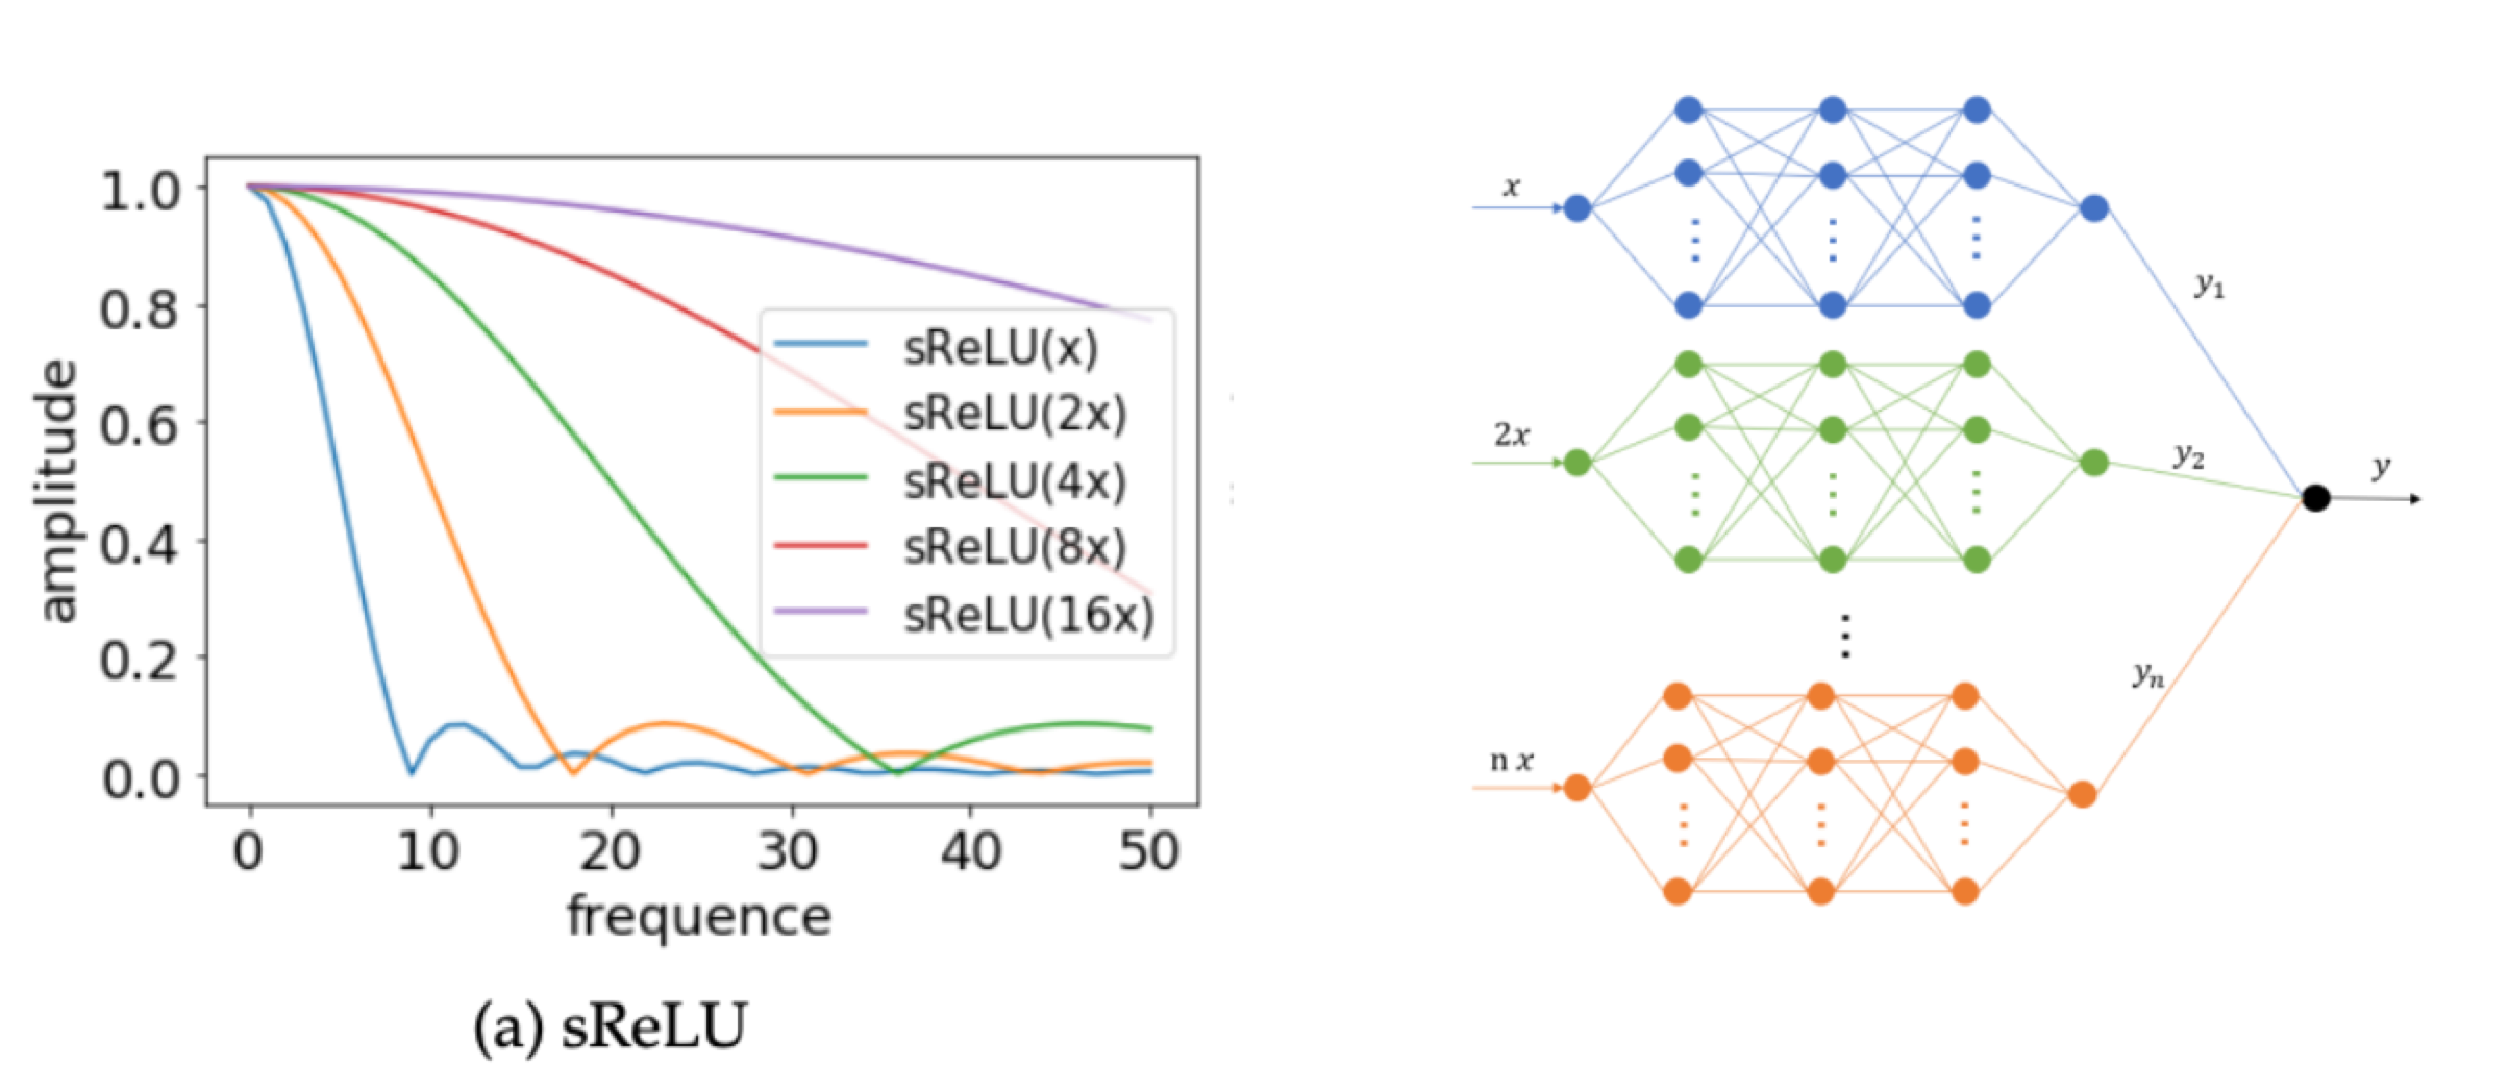
\includegraphics[scale=0.2]{figures/mscale.pdf}
\end{figure}



 
				
			

 
						
\end{itemize}
\end{itemize}  
%Important: \textcolor{magenta}{simultaneous} training of the complete network
\end{frame}




 
				
				















 \begin{frame}{A multigrid inspired  BCD training algorithm}
 %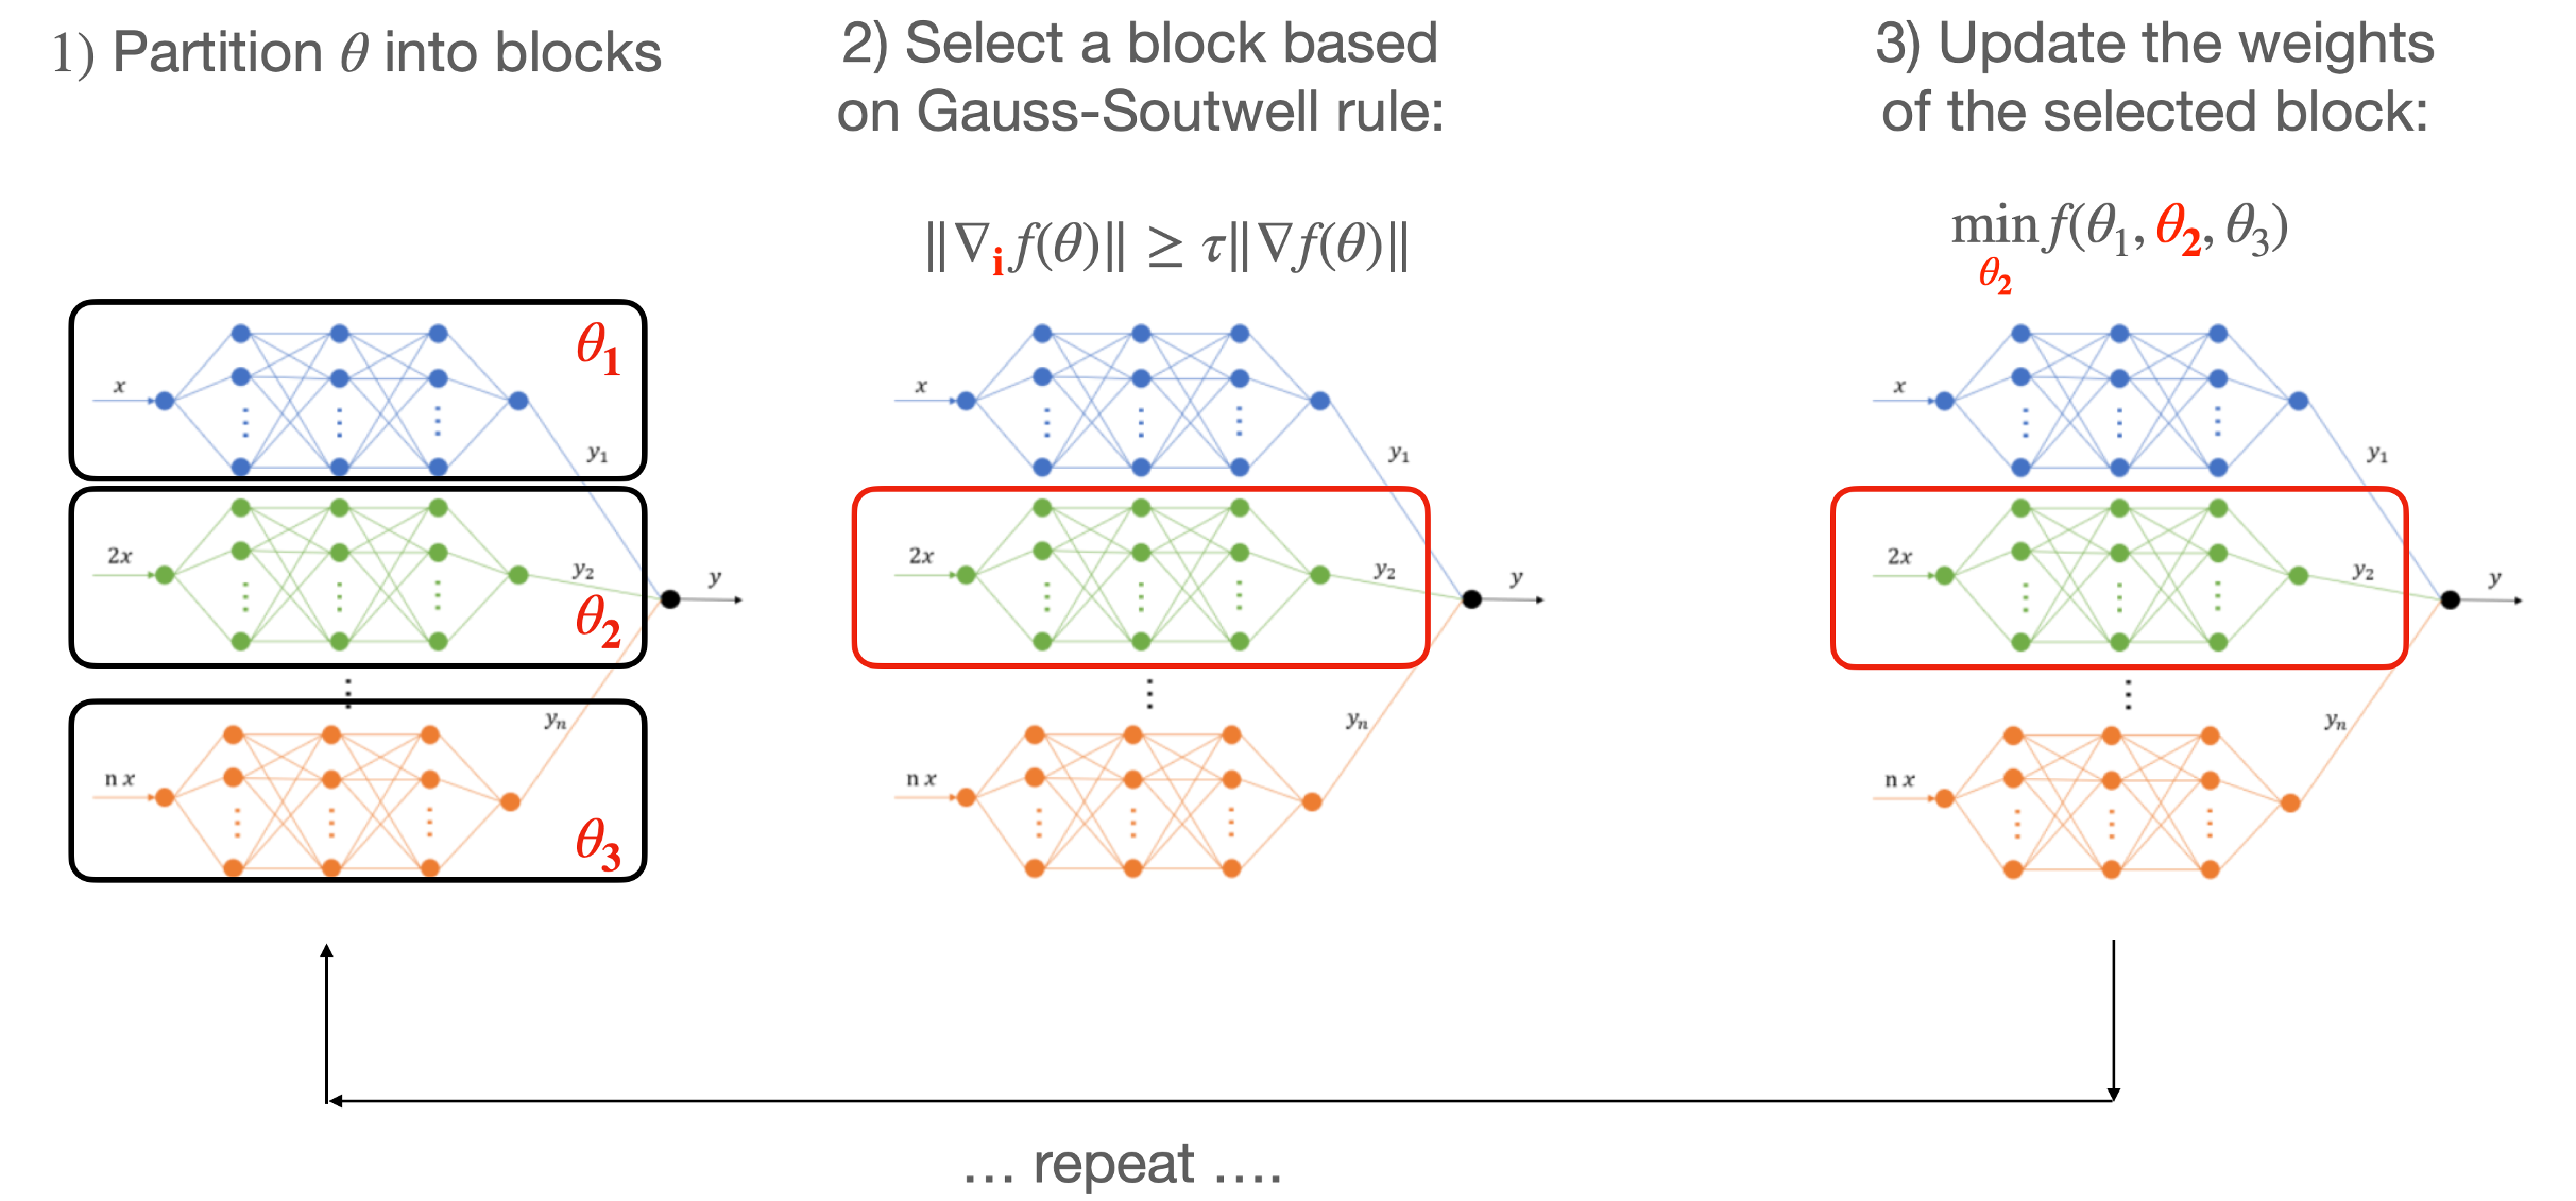
\includegraphics[width=\textwidth]{figures/MG_BCD}
% 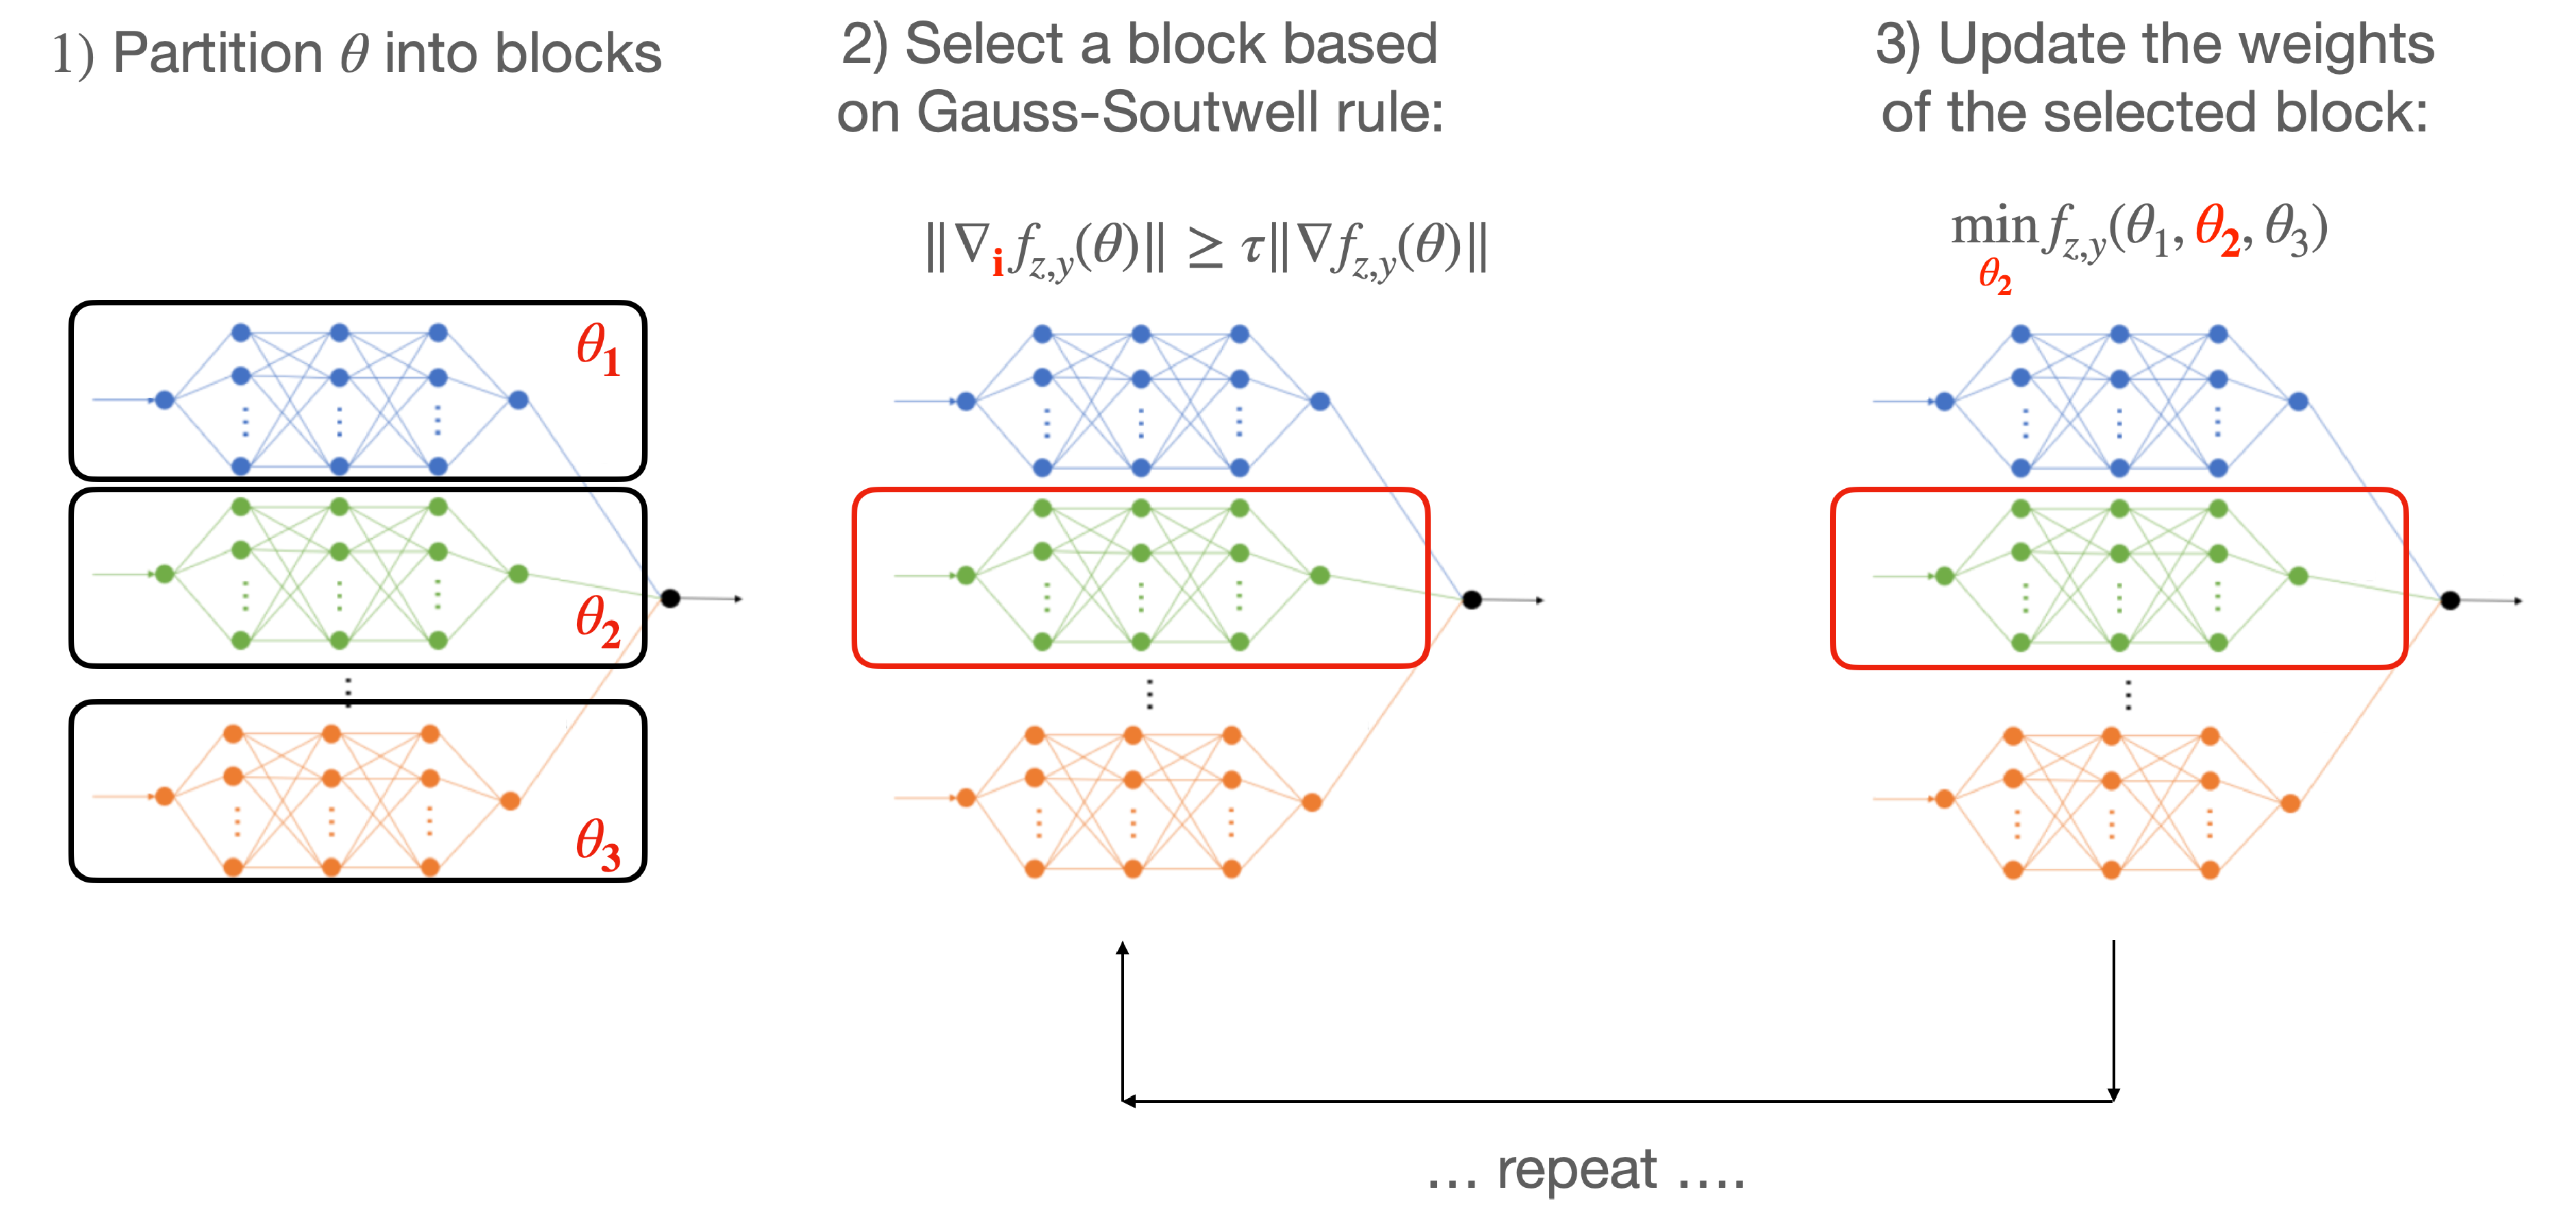
\includegraphics[width=\textwidth]{figures/schema_BCD}
 \includegraphics[width=\textwidth]{figures/BCD_MG}
 
 	\begin{tcolorbox}[
        title={Theoretical results},
    colback=green!10,
    colframe=green!70!black,
        fonttitle=\bfseries,
]

				\begin{itemize}
		\item Complexity ($O(\epsilon^{-2})$) in the deterministic and stochastic cases
		\end{itemize}



		
		

\end{tcolorbox}
 \small{\textcolor{mygreen}{[Gratton, Mercier, R., Toint, COAP, 2024]}}

 \end{frame}


\begin{comment}
 \begin{frame}{A multigrid inspired  BCD training algorithm}
$$\min_x f(x)$$
\centering

%\begin{minipage}{0.6\textwidth}
\begin{enumerate}
\item[1] Partition $x$ in blocks: \\
\includegraphics[width=0.4\textwidth, trim=1.5cm 0 0 0, clip]{images/step1}
\pause
\item[2] Select a block ${\color{red}i}$ $(x_1,\dots,{\color{red}x_i},\dots,x_n)$
\begin{itemize}
\item Criterion:   $\|\nabla_{\color{red}i}f(x)\|\geq \tau \|\nabla f(x)\|$,  $\tau\in(0,1)$
\end{itemize}
\includegraphics[width=0.4\textwidth, trim=1.5cm 0 0 0, clip]{images/step2}
\pause
 \item[3] Update the block: 
 \begin{itemize}
 \item  {\color{red}$p_k$} iterations of  a first-order method (possibly \textit{stochastic})
$$\min_{\color{red} x_i} f(x_1,\dots,{\color{red} x_i},\dots,x_n)\rightarrow x_i^{new}$$
\item ${\color{red}x_i}\leftarrow {\color{red}x_i^{new}}$ 

%\includegraphics[width=0.4\textwidth, trim=1.5cm 0 0 0, clip]{images/step3}

\end{itemize}

\end{enumerate}
%\end{minipage}
%\begin{minipage}{0.3\textwidth}
%\includegraphics[width=\textwidth]{images/BCD}

%\end{minipage}

\end{frame}
\end{comment}

\begin{comment}
\begin{frame}{A BCD-MG algorithm: convergence theory}
%\begin{columns}
%\begin{column}{0.5\textwidth}
\begin{theorem}
If $f$ has $L$-Lipschitz continuos gradient, the step-size $\alpha_k=\alpha<1/L$ and $p\leq p_{\max}$
\begin{itemize}
\item {\bf Deterministic}
$$
{\small \|\nabla f(x^{(K)})\|\leq \epsilon \rightarrow K=O\left(\frac{1}{\epsilon^2\alert{p}}\right)}
$$
%\end{column}
%\begin{column}{0.5\textwidth}
\item {\bf Stochastic}
$$
{\small \mathbb{E}\left(\sum_{k=1}^K\|\nabla f(x^{(k)})\|^2\right)\leq C_1(\sigma^2) + O\left(\frac{1}{K}\right)-C_2(\sigma^2)\alert{p}}
$$
%\end{column}
%\end{columns}
\end{itemize}
$p$ coarse iterations, $\sigma^2$ variance of stochastic gradient
\end{theorem}

\small{\textcolor{mygreen}{[Gratton, Mercier, R., Toint, COAP, 2024]}}
	
	
	
\end{frame}
\end{comment}

\begin{comment}
\begin{frame}{BCD-MG training of PINNs}
\centering

\begin{figure}
    \centering
 \only<2> {\includegraphics[width=0.6\linewidth]{images/training_1.png}}
  \only<3> {\includegraphics[width=0.6\linewidth]{images/training_2.png}}
   \only<1> {\includegraphics[width=0.6\linewidth]{images/training_3.png}}

\end{figure}
\end{frame}
\end{comment}






\begin{frame}{Numerical results: final MSE on average (10 runs)}
 
\begin{figure}
%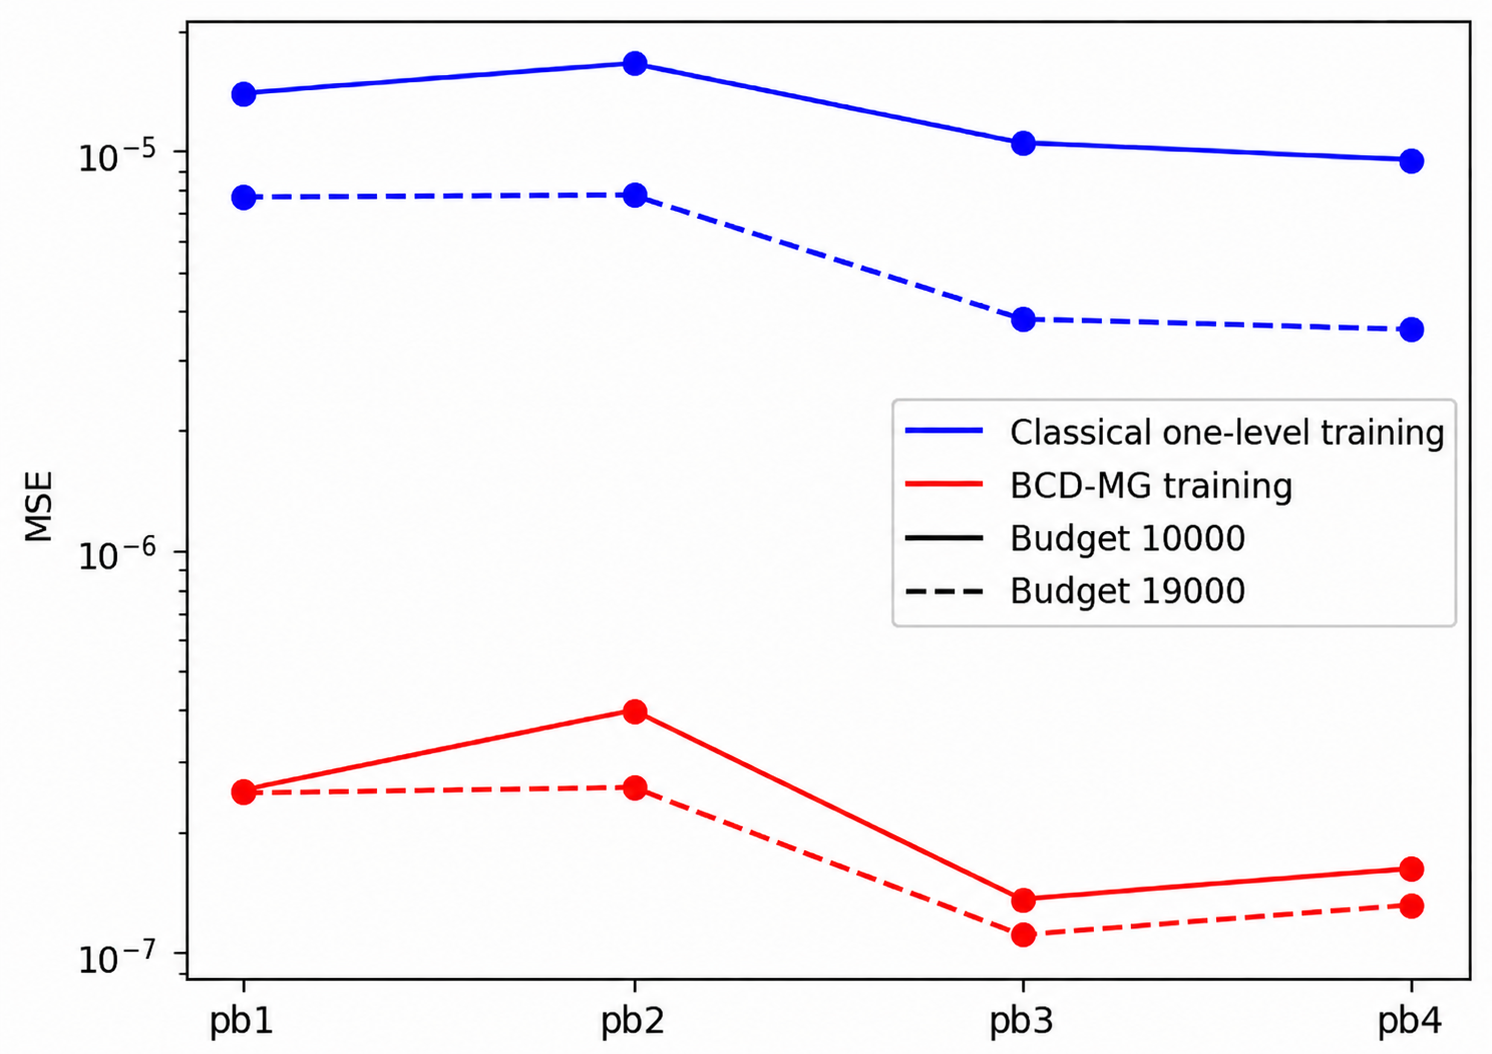
\includegraphics[width=0.45\linewidth]{figures/graph_poisson_new}
%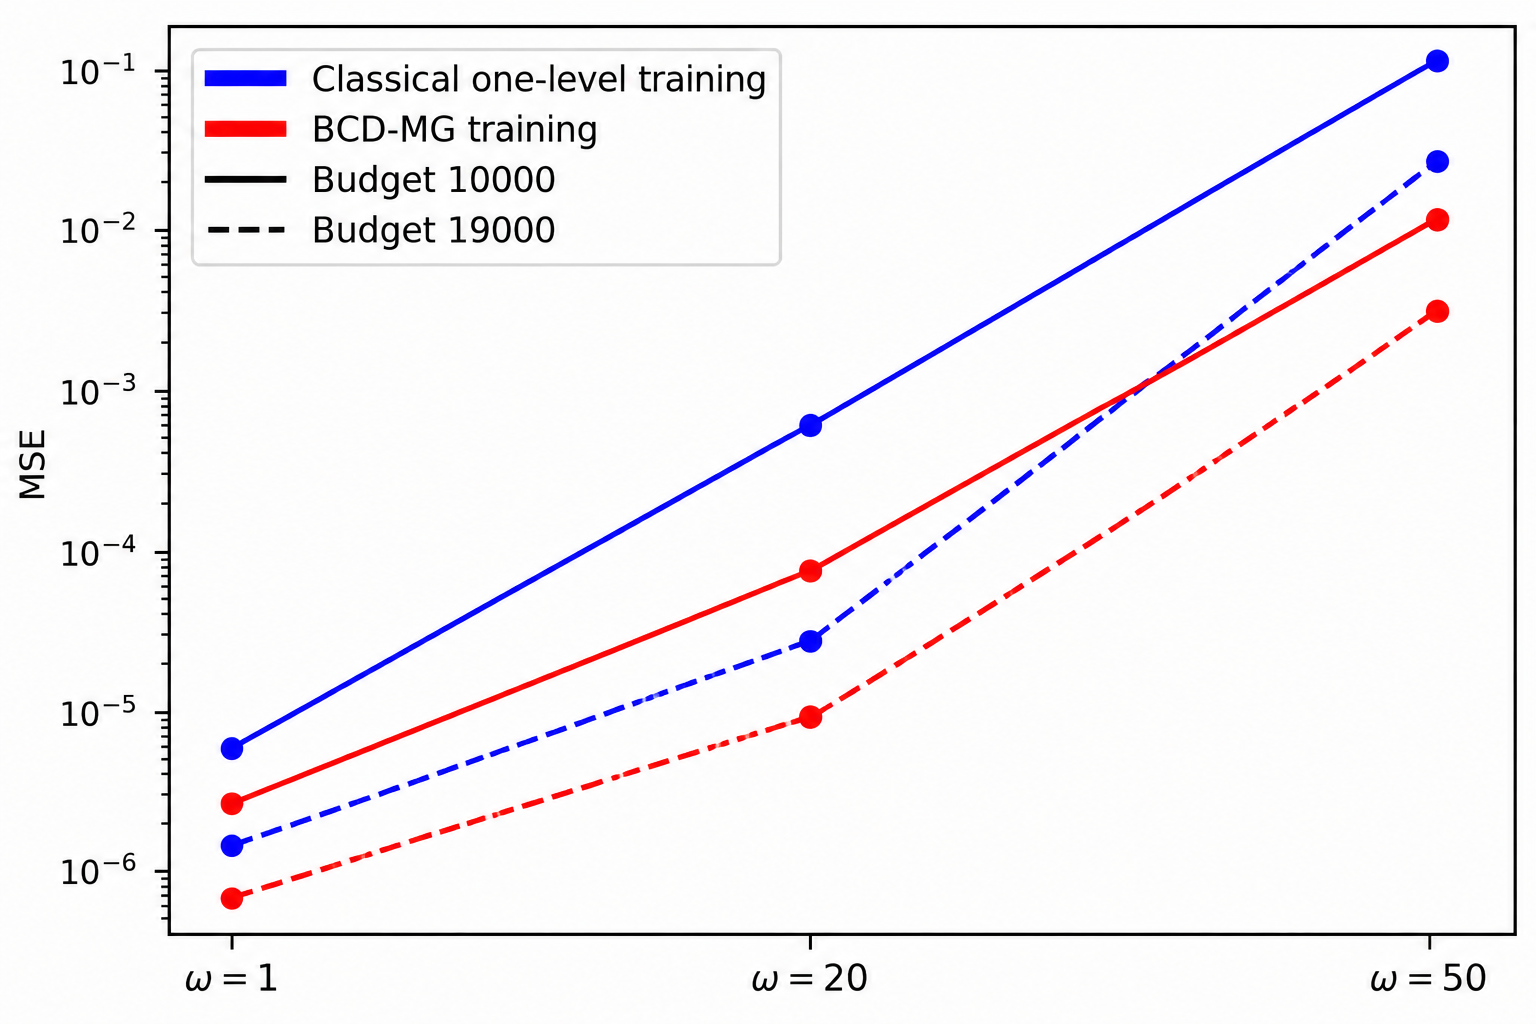
\includegraphics[width=0.45\linewidth]{figures/graph_heat_new}
%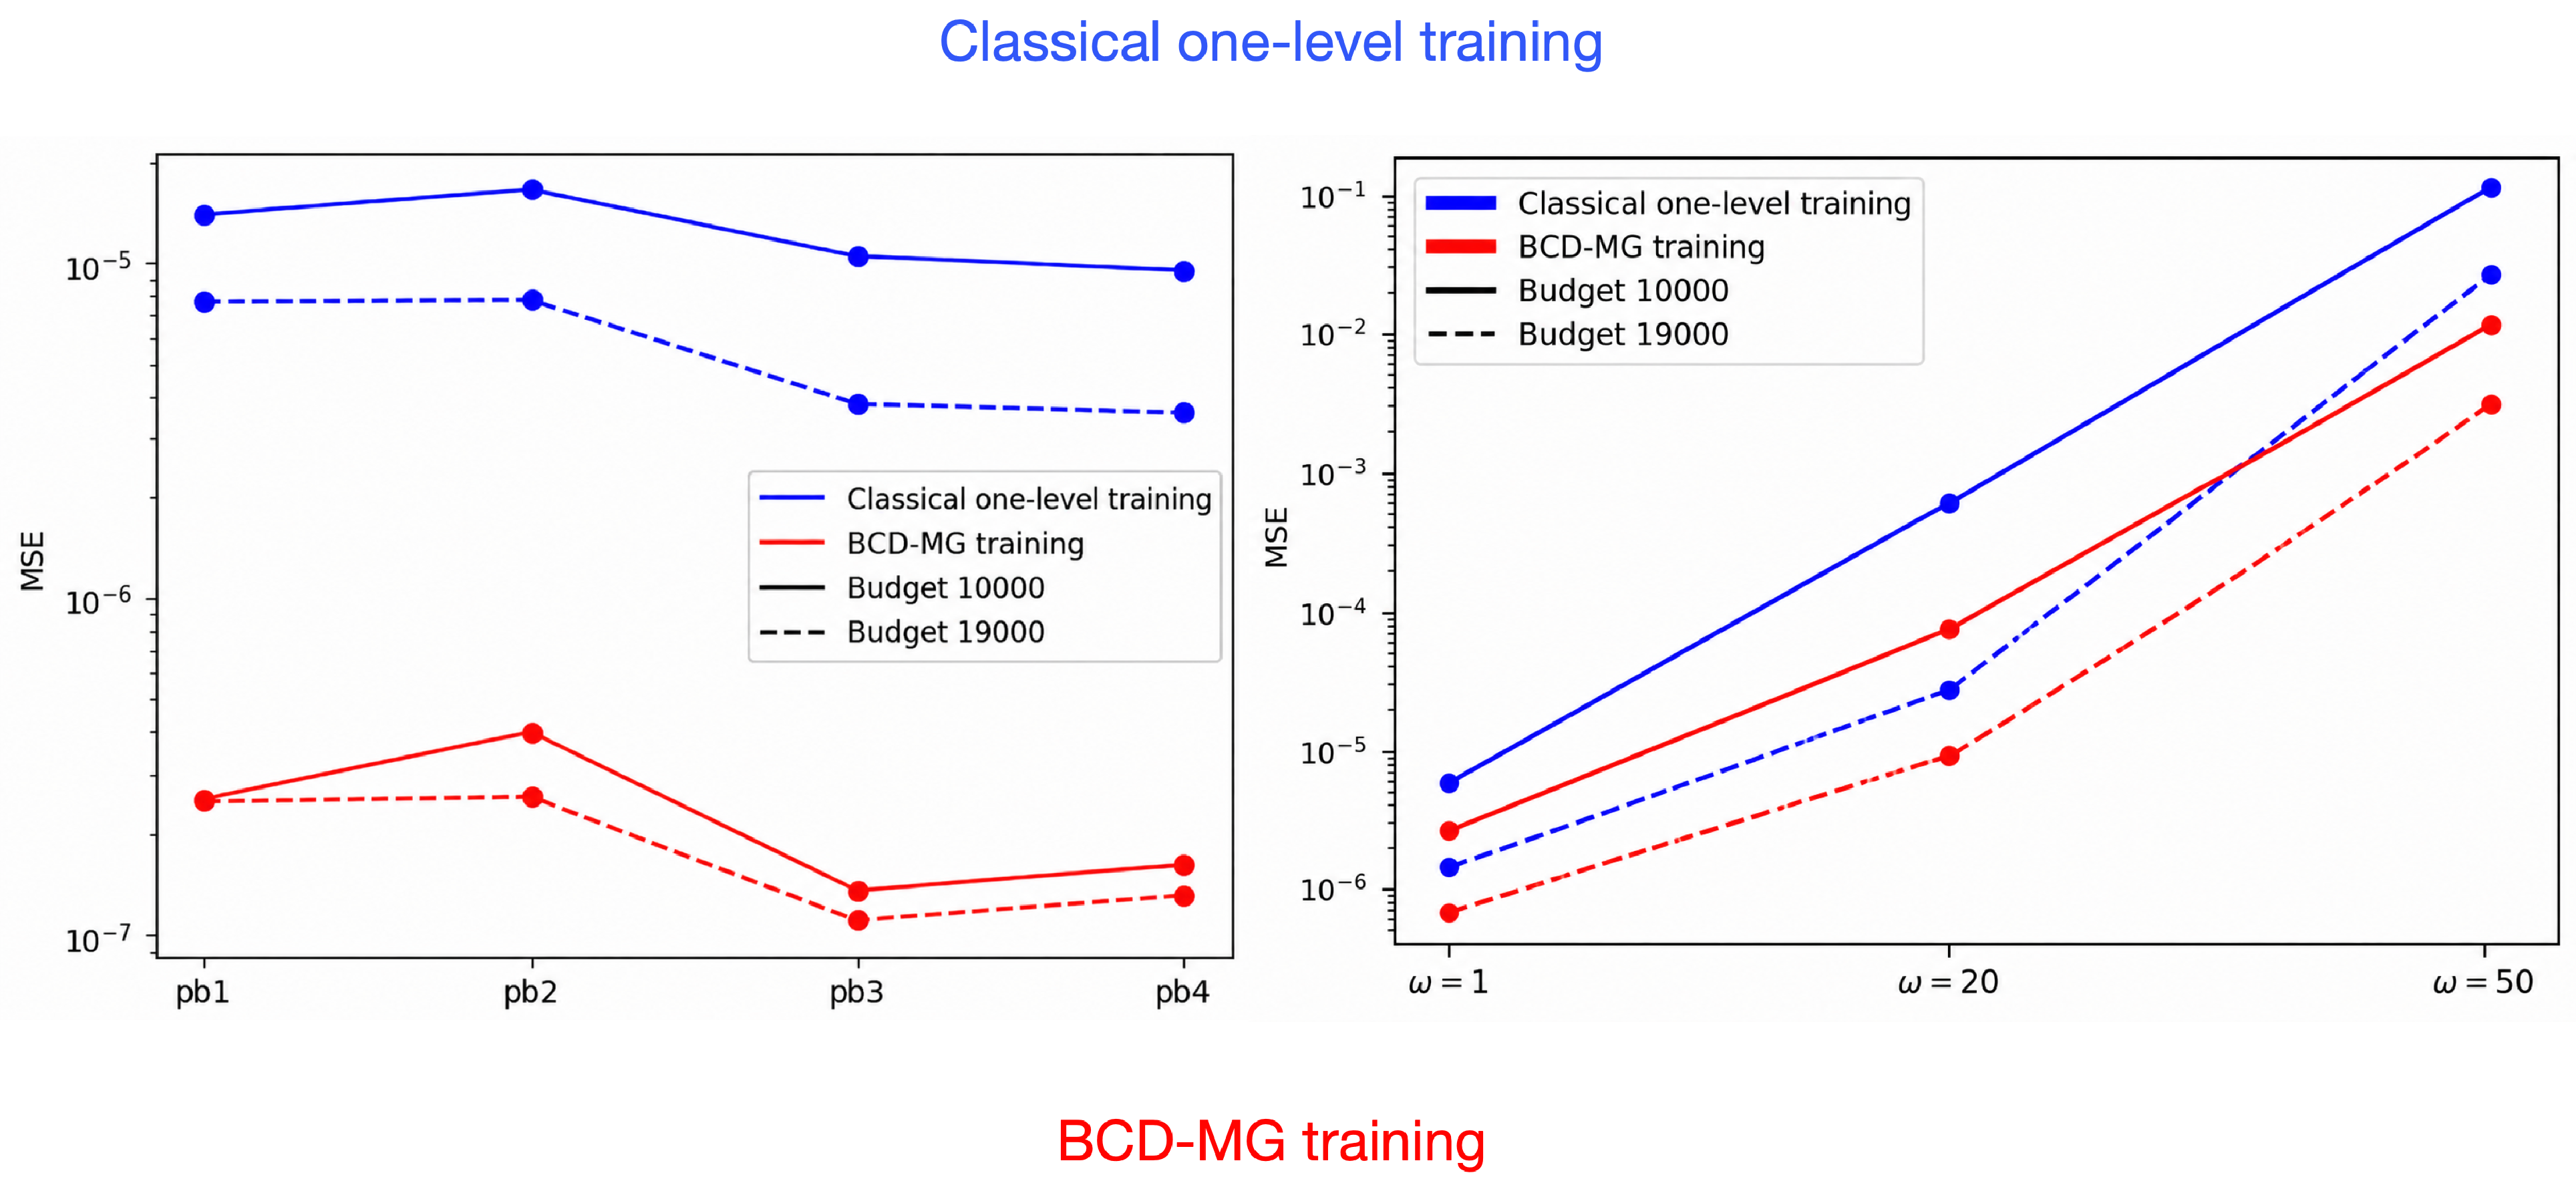
\includegraphics[width=\linewidth]{figures/exp_mscale}
%\includegraphics[width=\linewidth]{figures/BCD_MG_plot}
%\includegraphics[width=\linewidth]{figures/BCD_MG_heat}
\includegraphics[width=\linewidth]{figures/BCD_MG_pb}

%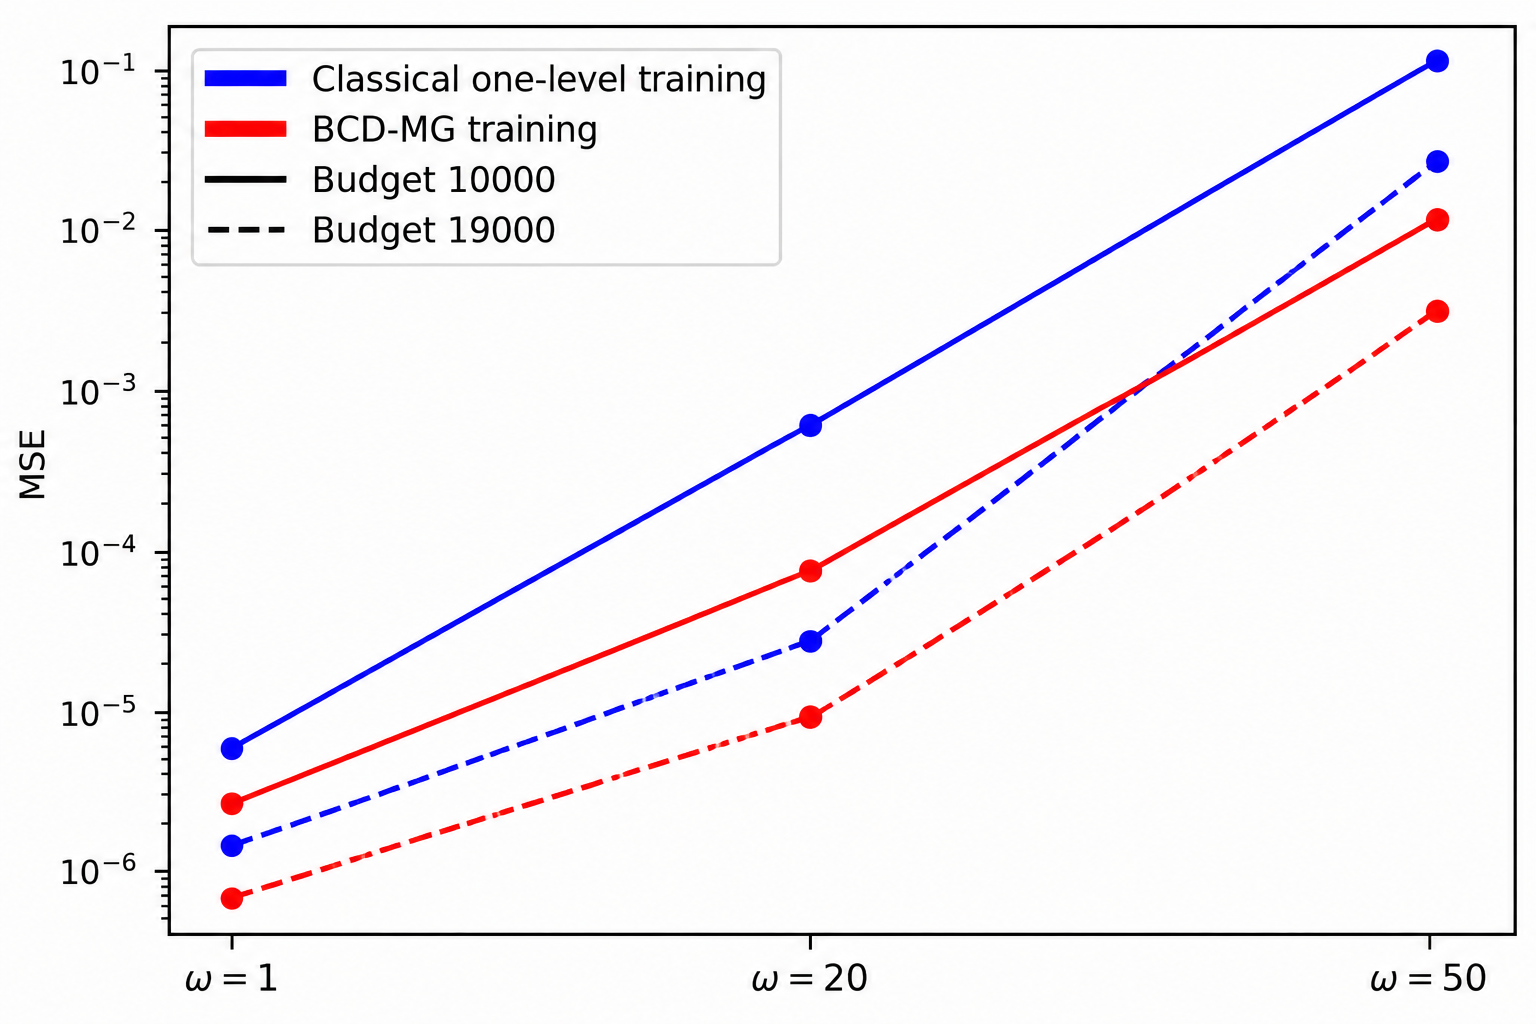
\includegraphics[width=0.45\linewidth]{figures/graph_heat_new}
\end{figure}

\end{frame}



    

\begin{comment}

\begin{frame}{(2) Expected risk minimization }
 $$
      \min_{\theta \in \mathbb{R}^n} \mathbb{E}_P[\mathcal{L}(m_z(\theta),y)]
$$
 
 \begin{itemize}
 \item
 Fine level: given $\{(z_i,y_i)\}_{i=1}^m\sim P$
 $$
\tilde f_k(\theta)=\frac{1}{|\mathcal{S}_k|}\sum_{i\in \mathcal{S}_k}f^{(i)}(x):= \mathcal{L}(m_{z_i}(\theta),y_i) \quad \theta\in\mathbb{R}^n, \quad \alert{|\mathcal{S}_k|\nearrow}
$$

\item Coarse level:
\end{itemize}
\begin{columns}
%====================================================
\begin{column}{0.48\textwidth}

\fbox{%
\begin{minipage}[t][0.4\textheight][t]{0.95\linewidth}

\centering

%\vspace{0.2cm}

{\bf Hierarchy in the function space at iteration $k$:}

%\vspace{0.2cm}

%Randomly draw
\begin{small}
\[
\mathcal{S}_k^1
\subseteq\dots\subseteq
\mathcal{S}_k^{\ell}
\subseteq\dots\subseteq
\mathcal{S}_k
\]
\end{small}
\vspace{-1cm}

%\vspace{0.2cm}

\begin{align*}
\tilde f_k(\theta)\approx 
\frac{1}{|\alert{\mathcal{S}_k^\ell}|}
\sum_{i\in\alert{\mathcal{S}_k^\ell}}
f^{(i)}(x)
\end{align*}

\end{minipage}%
}
\end{column}

%====================================================
\begin{column}{0.48\textwidth}


%\begin{minipage}[t][0.4\textheight][t]{0.95\linewidth}

\centering

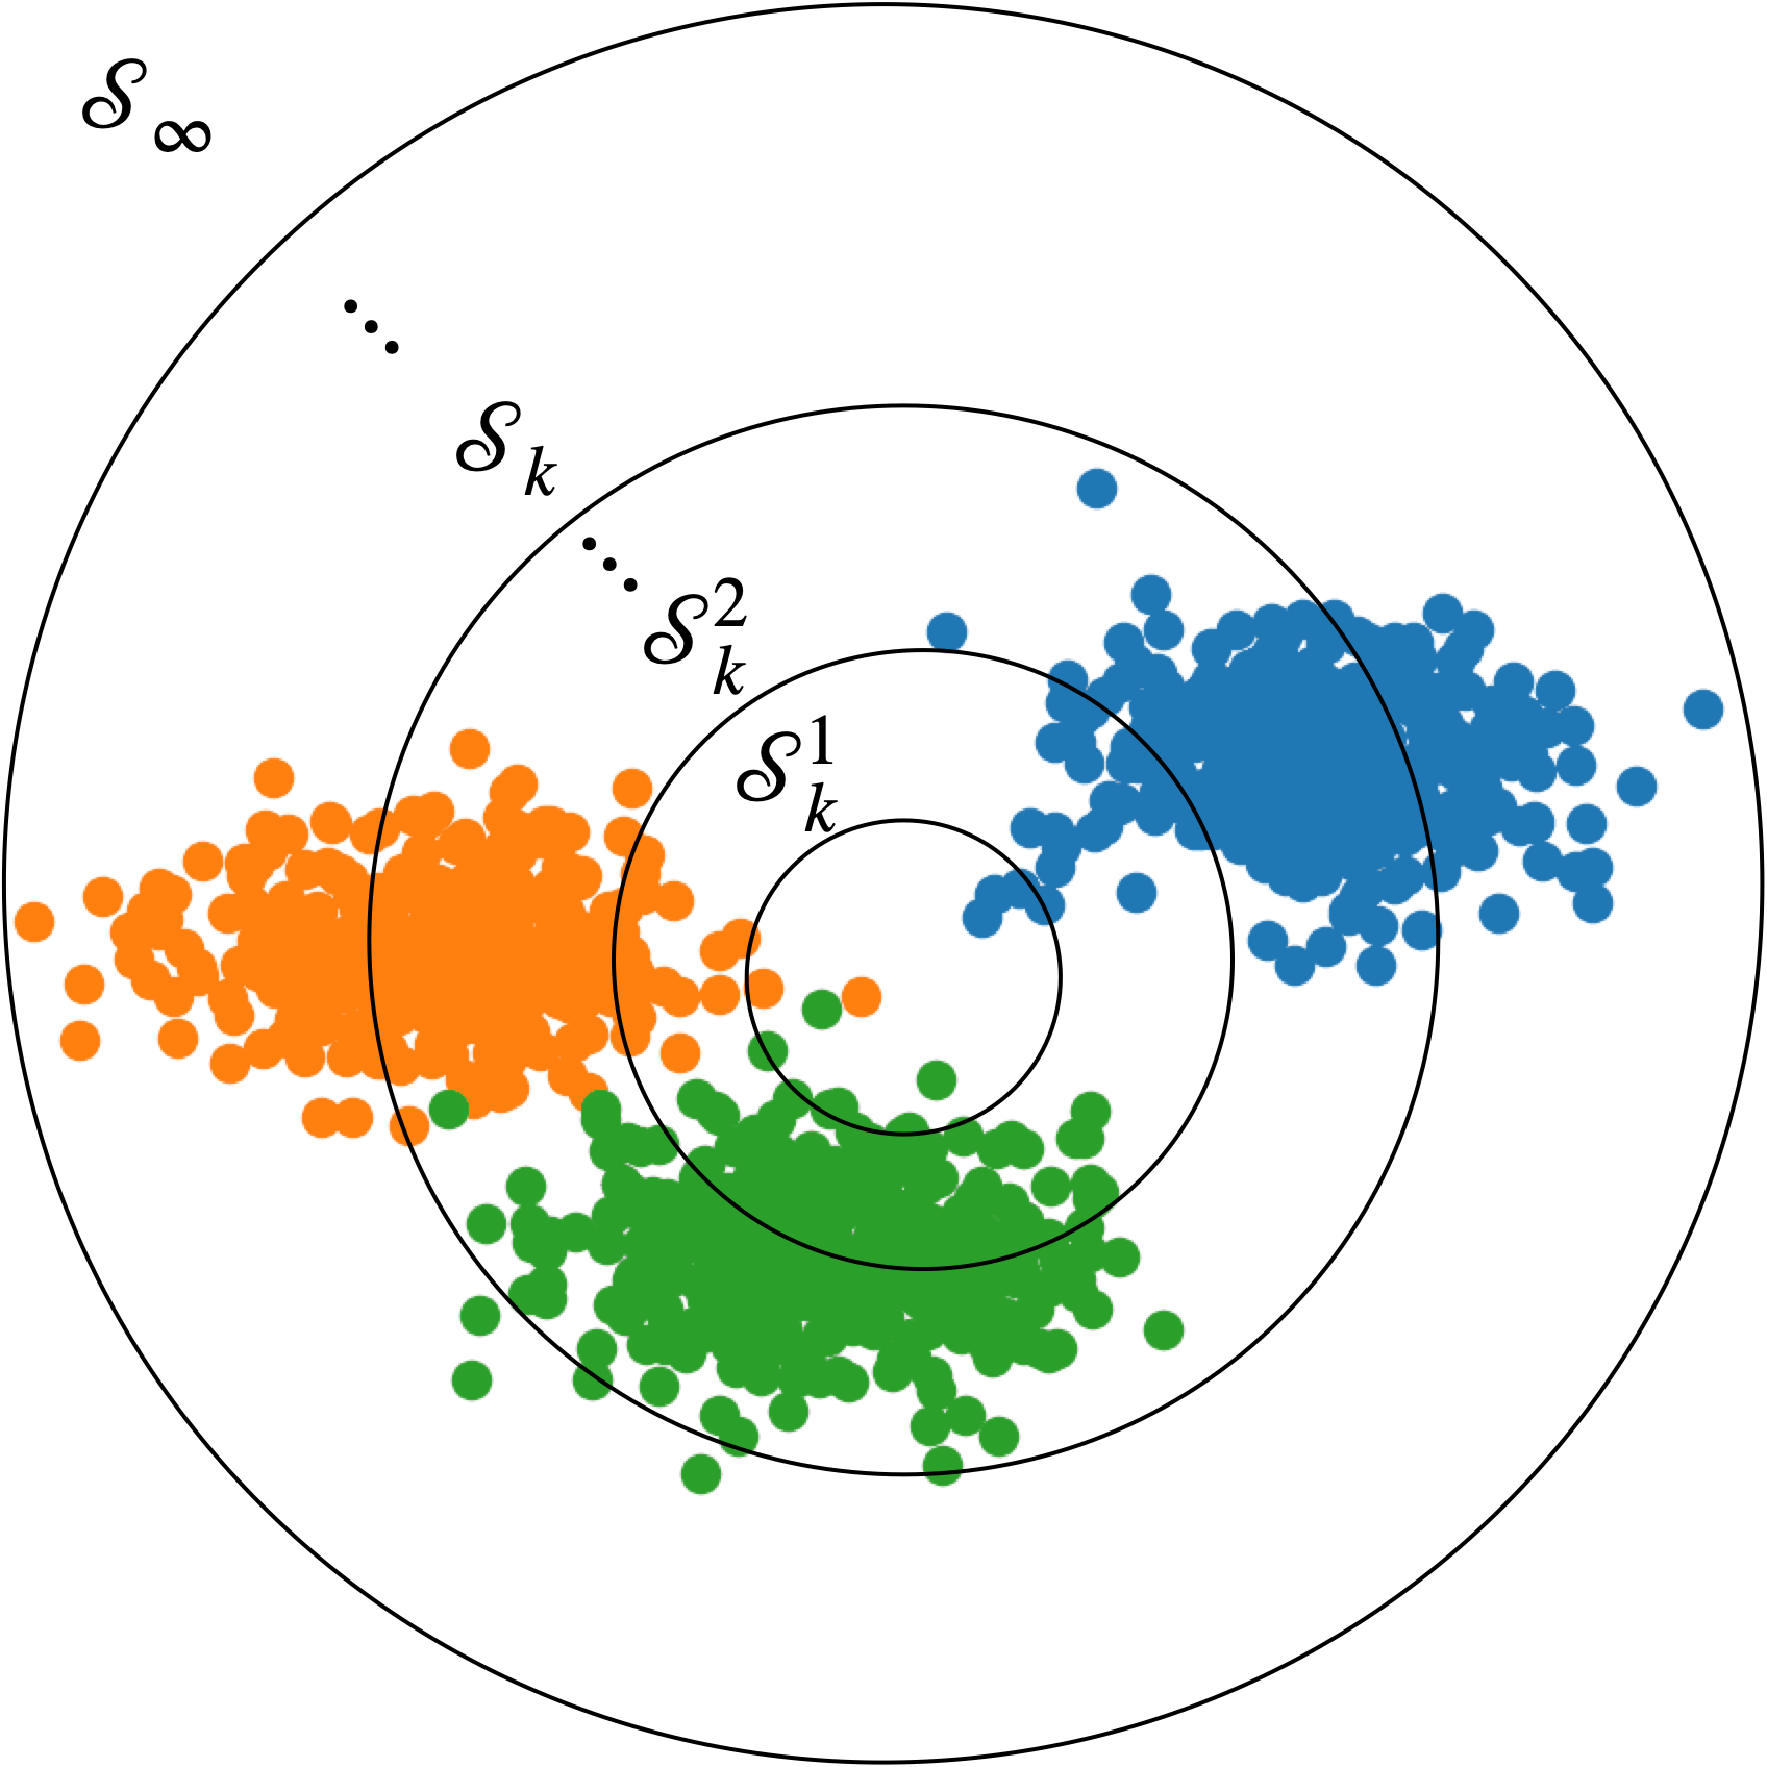
\includegraphics[width=0.9\textwidth]{figures/hierarchy_samples}
%\end{minipage}%






\end{column}

%====================================================
\end{columns}  
\end{frame}
\end{comment}
\begin{comment}
\begin{frame}{(2) Expected risk minimization }
 $$
      \min_{x \in \mathbb{R}^n} \mathbb{E}_P[\mathcal{L}(m_x(z),y)] \quad \text{stochastic problem}
$$
 
 \begin{itemize}
 \item
 Fine level: given $\{(z_i,y_i)\}_{i=1}^m\sim P$
 $$
\tilde f_k(x)=\frac{1}{|\mathcal{S}_k|}\sum_{i\in \mathcal{S}_k}f^{(i)}(x):= \mathcal{L}(m_x(z_i),y_i) \quad x\in\mathbb{R}^n, \quad \alert{|\mathcal{S}_k|\nearrow}
$$

\item Coarse level:
\begin{columns}

%====================================================
\begin{column}{0.48\textwidth}

\fbox{%
\begin{minipage}[t][0.4\textheight][t]{0.95\linewidth}

\centering

\vspace{0.2cm}

{\bf Hierarchy in the variables space at iteration $k$:}

%\vspace{0.2cm}
\vspace{-0.8cm}

%Randomly draw
\begin{small}
\[
\mathcal{V}^0
\subseteq\dots\subseteq
\mathcal{V}^\ell
\subseteq\dots\subseteq
\mathcal{V}^{\ell_{\max}}
\subseteq\mathbb{R}^n
\]
\end{small}

\vspace{-0.6cm}

\begin{align*}
\phi_k^\ell(\alert{x^\ell})
&=
\frac{1}{|\mathcal{S}_k|}
\sum_{i\in\mathcal{S}_k}
f^{(i)}(\alert{x^\ell})
\\
\alert{x^\ell} &\alert{\in \mathcal{V}^{\ell}}
\end{align*}

\end{minipage}%
}

\end{column}

%====================================================
\begin{column}{0.48\textwidth}

\fbox{%
\begin{minipage}[t][0.4\textheight][t]{0.95\linewidth}

\centering

\vspace{0.2cm}

{\bf Hierarchy in the function space:}

%\vspace{0.2cm}
\vspace{-0.8cm}

%Randomly draw
\begin{small}
\[
\mathcal{S}_k^0
\subseteq\dots\subseteq
\mathcal{S}_k^{\ell}
\subseteq\dots\subseteq
\mathcal{S}_k^{\ell_{\max}}
\subseteq\mathcal{S}_k
\]
\end{small}
\vspace{-1cm}

%\vspace{0.2cm}

\begin{align*}
\phi_k^\ell(x)
&=
\frac{1}{|\alert{\mathcal{S}_k^\ell}|}
\sum_{i\in\alert{\mathcal{S}_k^\ell}}
f^{(i)}(x)
\\
x &\in \mathbb{R}^n
\end{align*}

\end{minipage}%
}

\end{column}

%====================================================
\end{columns}  
\end{itemize}\end{frame}



\begin{frame}{Numerical results }

\begin{figure}[h!]
    \centering
    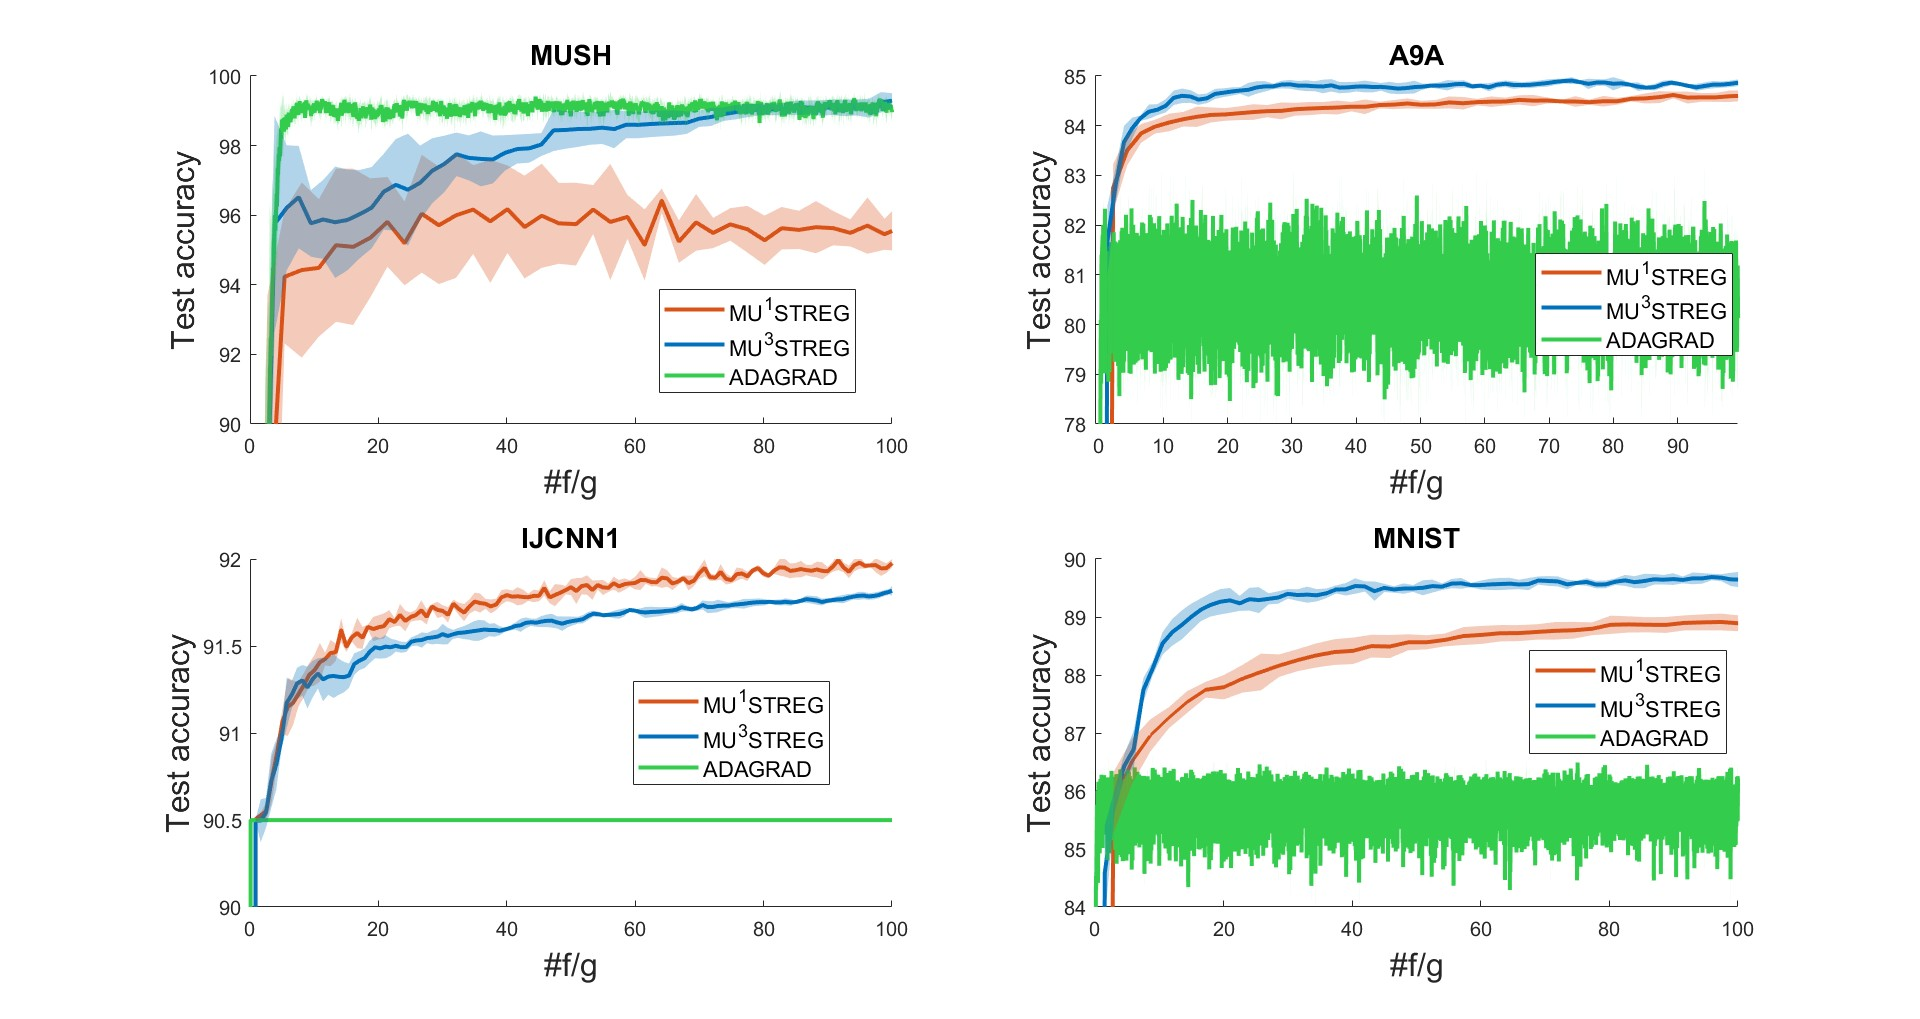
\includegraphics[width=\linewidth]{figures/LEAST-SQUARES_acc_vs_ev_SHADED.jpg}
    \caption{ Test accuracy vs number of  weighted evaluations of gradients and functions.}
    \label{fig: acc vs. ev.}
\end{figure}
	
	\end{frame}


\end{comment}






	
	\part{Exploiting hierarchies  of structured matrices  }
	\frame[plain]{\partpage}
	
	\begin{frame}
\frametitle{Sparse matrix factorization}
Given a dense matrix $A$, find \emph{sparse} factors $S_1, S_2, \ldots, S_J$ s.t.: 
		$$A \approx S_1 S_2 \ldots S_J$$
				\pause 
		





\vspace{-0.2cm}
\begin{itemize}		
			\item    Fast Fourier Transform, Fast Hadamard Transform, etc.
			
	\end{itemize}

	\begin{figure}
		\includegraphics[scale=0.2]{FastFourierTransform.png}
		%\caption{The factorization of the Discrete Fourier Transform.}
	\end{figure}
	\begin{tiny} 
				\textcolor{gray}{[J. W. Cooley, J. W. Tukey, 1965]}
				\end{tiny}




	\begin{tcolorbox}[title = \textbf{Sparse matrix factorization problem}]
		Given a matrix $A$ and $\mathcal{E}_j$ sets of sparse matrices, solve:
		\setlength{\abovedisplayskip}{0pt}
		\begin{equation*}
			%\begin{aligned}
				%\label{eq:sparse_recovery1}
				\underset{S_1, \ldots , S_J}{\min}  \|A - \prod_{j = 1}^J S_j\|_F^2   \;
				\text{ subject to: } \; S_j \in \mc{E}_j,   \forall j \in \{1, \ldots, J\} 
		%	\end{aligned}
		\end{equation*}
	\end{tcolorbox}

			\begin{tiny}
	\textcolor{gray}{[J. Malik,   2017]}, 
	\textcolor{gray}{[S. Foucart, H. Rauhut,  
2013]}
\end{tiny}


\centering A very hard problem! 
\end{frame}






	


\begin{frame}{Two-factors fixed support matrix factorization}
		
	
	%$\rightarrow$ Inheritance from great literature of matrix decomposition problems
			\begin{tcolorbox}
			%\begin{tcolorbox}[title = \text{2) Optimize coefficients inside support}, colframe =  red!70!yellow, colbacktitle= red!70!yellow]
			\setlength{\abovedisplayskip}{0pt}
			\begin{equation*}\tag{FSMF}
				\begin{aligned}
					& \min_{X \in \mb{R}^{m \times r}, Y \in \mb{R}^{n \times r}}
					& &L(X, Y) = \|A - XY^\top\|_F^2&\\
					& \text{Subject to: }
					& &\texttt{supp}(X) \subseteq S_X&\\
					& & &\texttt{supp}(Y) \subseteq S_Y&\\
				\end{aligned}
			\end{equation*}
		\end{tcolorbox}

		%\onslide<3>{\textcolor{red}{$\rightarrow$ It can be seen as a sparse linear neural network of two layers.}}

		
	%	\colorbox{red}{\textcolor{white}{Fixed support matrix factorization}} covers several existing frameworks:
	
				
		\begin{itemize}
					\item Low rank matrix decomposition
			\item LU decomposition
			%\item Hierarchical $\mc{H}$ and BLR matrices
			\item Butterfly factorization
		\end{itemize}
	
		
		
		

		
		\begin{figure}[h]
			\centering
			\includegraphics[scale=0.26]{lmra_lu.png}
			\end{figure}
			\begin{figure}[h]
			\centering
			\includegraphics[scale=0.26]{hadamard}
		\end{figure}
		
		
		\end{frame}
		
		

			
			
     
 
 
 \begin{comment}
 \begin{frame}{Main questions for \textcolor{red}{FSMF}}
		\begin{itemize}
			\item[1)] Is it polynomially tractable?
			
			\item[2)] Otherwise, are there easy instances?
			
			\item[3)] How well does gradient descent tackle the problem of FSMF?
		\end{itemize}
\end{frame}
\end{comment}


%\section{Main Results}
%\frame{\tableofcontents[currentsection]}

\begin{frame}{My contributions}
		
		\begin{enumerate}
				\item The problem is   \textcolor{red}{NP-hard}.
		\vfill
		
		\item The problem has an  \textcolor{red}{essentially unique solution} in the exact case

\vfill

		
		\item \alt<2->{  \fbox{\parbox{0.85\textwidth}{There is a family of \textcolor{red}{polynomially solvable} instances and  an  \textcolor{red}{efficient algorithm} to solve them}}
}{There is a family of \textcolor{red}{polynomially solvable} instances and  an  \textcolor{red}{efficient algorithm} to solve them}
		
		\vfill
		\item Some properties of the \textcolor{red}{landscape} of the function $L(X,Y) = \|A - XY^\top\|^2$ \emph{under the support constraints} are known, which help to understand how well \emph{gradient descent} tackles the problem of FSMF
		
		
		
	\end{enumerate}
			
			\vspace{0.2cm}
		 \footnotesize{ \textcolor{mygreen}{[Zheng, R., Gribonval, SIMODS, 2023]}}, 
 \footnotesize{ \textcolor{mygreen}{[Le, R., Gribonval, SIMAX, 2023] }}
					
	
\end{frame}



\begin{comment}
\begin{frame}{A polynomially solvable instance: unconstrained MF }


	\begin{columns}[c]

\begin{column}{0.48\textwidth}
\[
\min_{X \in \mathbb{R}^{m \times r},\, Y \in \mathbb{R}^{n \times r}}
L(X,Y)
=
\|A-XY^\top\|_F^2
\]
\end{column}

\begin{column}{0.48\textwidth}
\centering
\includegraphics[width=0.8\linewidth]{lowrankapprox.pdf}
\end{column}

\end{columns}	
\vspace{0.3cm}
	$\rightarrow$ \textcolor{red}{Solution: Use Singular Value Decomposition (SVD).}
\pause
	\begin{itemize}
		\item[1)] Decompose the problem:
		\begin{equation*}
			A - XY^\top = A - \sum_{i = 1}^r x_iy_i^\top = A - \sum_{i = 1}^r \underbrace{M_i}_{\text{rank-one}} \quad (M_i := x_iy_i^\top)
		\end{equation*}
		\vspace{-10pt}
		\pause
		\item[2)] Finding the SVD:
		\begin{equation*}
			\begin{aligned}
				&\texttt{bestRankOneApprox}(A) &\to  M_1\\
				&\texttt{bestRankOneApprox}(A - M_1) &\to  M_2\\
				&\cdots&\\
				&\texttt{bestRankOneApprox}(A - M_1 \ldots - M_{r-1}) &\to M_r
			\end{aligned}
		\end{equation*}
	%	\pause
	%	$\rightarrow$ \textcolor{red}{SVD is a greedy algorithm in disguise}
			\end{itemize}
\end{frame}
\end{comment}


\begin{frame}{A greedy SVD algorithm}

    \begin{itemize}

        \item Decompose $XY^\top$:
        \[
            XY^\top
            = \sum_{i=1}^r x_i y_i^\top
            = \sum_{i=1}^r \underbrace{M_i}_{\text{rank-one}}
            \qquad (M_i := x_i y_i^\top)
        \]
         \item Finding the SVD:
        \end{itemize}

\begin{columns}
\begin{column}{0.5\textwidth}

		\begin{equation*}
		\begin{footnotesize}
			\begin{aligned}
				&\texttt{Rank1Approx}(A) &\to  M_1\\
				&\texttt{Rank1Approx}(A - M_1) &\to  M_2\\
				&\cdots&\\
				&\texttt{Rank1Approx}(A - \sum_{i=1}^{r-1}M_i) &\to M_r
			\end{aligned}
			\end{footnotesize}
		\end{equation*}
      

            \end{column}
            \begin{column}{0.5\textwidth}
           
 \begin{figure}
            \foreach \n in {4}{
                \includegraphics[
                    width=0.8\textwidth,
                    page=\n
                ]{rank1contribution.pdf}
            }
                    \end{figure}
            \end{column}
            \end{columns}

\vspace{0.2cm}
       \begin{itemize}
		\item 
		The solution will always \emph{satisfy the constraints}
		\item It may NOT be \emph{optimal}
				\end{itemize}


\end{frame}

\begin{comment}
\begin{frame}{}
\begin{algorithm}[H]
			\centering
\caption{Algorithm for fixed-support matrix factorization}\label{algorithm1}
			\begin{algorithmic}[1]
				\setlength{\belowdisplayskip}{0pt}
				\For {$i \in \{1,\ldots,r\}$}	
				\State $S_i$ $\leftarrow$ $i$-th rank-one support 
								\State $M_i: = $ best rank-one approximation of $(A - \sum_{k = 1}^{i - 1} M_k)\odot S_i$
				\EndFor
			\end{algorithmic}
		\end{algorithm}
		
		\begin{figure}
		\foreach \n in {1,2,3,4}{\includegraphics<beamer|\n>[scale=0.4, 
			page=\n]{algorithmillu.pdf}}
	\end{figure}
		
		
		
\end{frame}
\end{comment}

\begin{frame}{Polynomial solvability characterized by rank-one supports}

	
		
	
	
		If the rank-one supports are \alert{pairwise disjoint or identical} the greedy algorithm gives an \alert{optimal solution}, even in the \emph{non-exact} case 
	

	


\begin{tcolorbox}{Notable case: butterfly matrices}
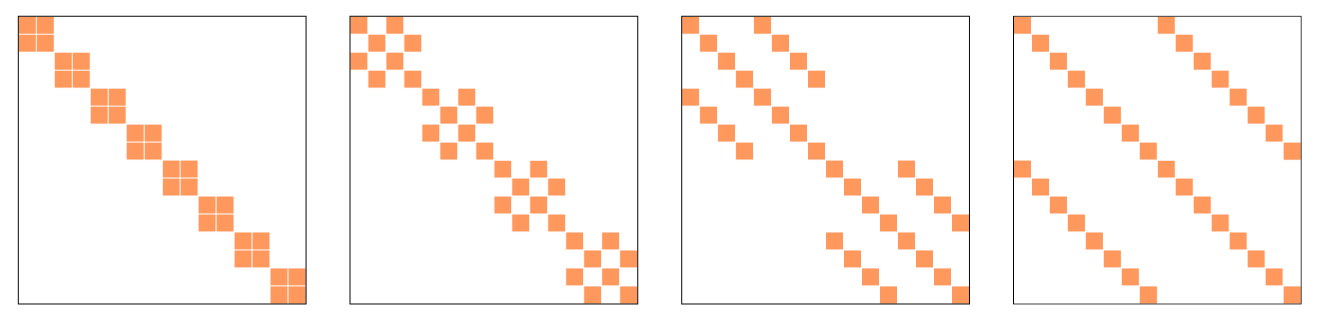
\includegraphics[width=\textwidth]{figures/butterfly_factors}
%\includegraphics[width=0.24\textwidth]{S_2}
%\includegraphics[width=0.24\textwidth]{S_3}
%\includegraphics[width=0.24\textwidth]{S_4}

\begin{itemize}
\item Butterfly matrices are extremely sparse yet highly expressive, they appear in many fast linear transforms
\item {\color{red}Butterfly factorization}: decompose dense $n\times n$ matrix as $B_1 \ldots B_L$, with $L=\log_2 n \Raw \text{matvec in } O(n\log n)$ 
\end{itemize}
\end{tcolorbox}
\end{frame}


\begin{comment}
\begin{frame}{Key property for butterfly factorization}
\begin{itemize}
\item
For any partial product $XY^T$ of consecutive factors
$$
B_1 \ldots B_{j} \underbrace{B_{j+1} \ldots B_{k}}_{X} \underbrace{B_{k+1} \ldots B_{\ell}}_{Y^T} B_{\ell+1} \ldots B_L
$$
\begin{columns}
\begin{column}{0.4\textwidth}
$$
XY^T = \sum_{i=1}^n x_iy_i^T
$$
where the rank-one matrices $x_iy_i^T$ have disjoint support.
\end{column}
\begin{column}{0.7\textwidth}

\includegraphics[width=\textwidth]{first_step1_new.pdf}
\end{column}
\end{columns}


\end{itemize}

\end{frame}
\end{comment}


\begin{frame}{Hierarchical algorithm for butterfly factorization}
	
		
		
		\begin{columns}
		\begin{column}{0.5\textwidth}
		%	Let $\mathbf{A} := \mathbf{X}^{(4)} \mathbf{X}^{(3)} \mathbf{X}^{(2)} \mathbf{X}^{(1)}$ 
			\begin{figure}
				\begin{overprint}
					\onslide<1>\centerline{\includegraphics[width=0.7\textwidth]{tree_partial_1}}
					\onslide<2>\centerline{\includegraphics[width=0.7\textwidth]{tree_partial_2}}
					\onslide<3->\centerline{\includegraphics[width=0.7\textwidth]{tree_3}}
					%\onslide<4->\centerline{\includegraphics[width=0.45\textwidth]{tree_1}}
				\end{overprint}
			\end{figure}
			\end{column}
\begin{column}{0.5\textwidth}

					Solve a sequence of \alert{two-factors} problems  
		
		
		\pause
		
		\onslide<4->{Works also with different kind of trees
		\begin{figure}
		\includegraphics[scale=0.2]{balanced_tree.png}
		\end{figure}}


	\end{column}
		\end{columns}

		\onslide<5->{	 \begin{tcolorbox}[
      title=Theoretical guarantees,
      colback=white,
      colframe=gray!40,
      boxrule=0.4pt,
      arc=4pt,
      left=6pt, right=6pt, top=4pt, bottom=4pt,
    ]
    \begin{columns}
    \begin{column}{0.48\textwidth}
    \begin{tiny}
	\begin{block}{\small Exact setting}
	\begin{itemize}
	\item
	The factorization  is \alert{essentially unique}
	\item The factors can be recovered by the algorithm.
	\end{itemize}

	 \end{block}
	 	 \end{tiny}
	 \end{column}
	 \begin{column}{0.48\textwidth}
	     \begin{tiny}

 \begin{block}{\small Noisy setting}
 \begin{itemize}
	\item The algorithm can approximate \alert{any} matrix by a matrix having the butterfly structure
	%But because this procedure is used in a recursive greedy fashion in Algorithm 3.1, 
	\item Global optimality  is \emph{not guaranteed}
	\end{itemize}
 \end{block}
	 \end{tiny}
 	 \end{column}

	 \end{columns}

 \end{tcolorbox}}
		
		\onslide<5->{ \small{ \textcolor{mygreen}{[Le, Zheng, R., Gribonval, ICASSP, 2022 and SIMAX, 2025]}}}
		  
	\end{frame}
	
\begin{comment}
	\begin{frame}{An important application: the butterfly factorization}
	
	\begin{block}{Theoretical guarantees? }
	In general we cannot guarantee optimality of the solution. 
	\end{block}
	\begin{block}{A special case: the butterfly factorization} 
	Approximate \textbf{any} matrix by a product of $J\geq 2$ \alert{butterfly} factors 
		\end{block}
	
	\vspace{0.5cm}
		
			Let $\mathbf{A} := \mathbf{X}^{(4)} \mathbf{X}^{(3)} \mathbf{X}^{(2)} \mathbf{X}^{(1)}$ such that:
			\begin{figure}
				\centering
				\includegraphics[scale=0.1]{butterfly_constraint}
			\end{figure}
			
			



						
		
		
	\end{frame}
	\end{comment}
	
	
	
	
	%\end{comment}
	


				

	
	
	
	

 
 
	
		

	\begin{comment}
	\begin{frame}\frametitle{Numerical results: 2 factors}
 $A$ the Hadamard matrix of size $2^J \times 2^J$, $J=10$, two different supports 
 % which is known to admit an exact factorization with each of the considered support constraints
%\begin{itemize}
%\item[a)] $I_1 =J_1= \mathbf{1}_{2^a \times 2^a} \otimes \mathbf{I}_{2^b\times 2^b}$;  b) $I_2 = \mathbf{1}_{2 \times 2} \otimes \mathbf{I}_{2^{N - 1}}, J_2 = \mathbf{I}_2 \otimes \mathbf{1}_{2^{N-1} \times 2^{N-1}}$\footnote{ supports used for the hierarchical approximation of a matrix by a product of $N$ butterfly factors} 
%\end{itemize}


\begin{figure}[bhtp]
	\label{fig:experment1}
	\includegraphics[scale=0.25]{hadamardten.png}
		\includegraphics[scale=0.25]{runningtime_size.png}

	%\caption{Evolution of $\log_{10} \|A - XY^\top\|_{F}$ for three variants of gradient descent and \Cref{algorithm3} with support constraints $(I_1,J_1)$ (left) and $(I_2, J_2)$ (right) for $N =10$.}
\end{figure}	

\end{frame}
\end{comment}

\begin{comment}
\begin{frame}\frametitle{Numerical results: DFT by $J=9$ butterfly factors}

\begin{columns}
\begin{column}{0.5\textwidth}
Faster and more accurate in the \alert{noiseless setting}

	
	\begin{figure}
		\centering
		\includegraphics[width=\textwidth]{DFT_exact}
	\end{figure}
	\end{column}
\begin{column}{0.5\textwidth}
Also more robust in the \\\alert{noisy setting}
	
	
	\begin{figure}
		\centering
		\includegraphics[width=\textwidth]{DFT_bruit}
	\end{figure}
	\end{column}
	\end{columns}
	
	 \begin{tcolorbox}[
      title=Practical advantages,
      colback=white,
      colframe=gray!40,
      boxrule=0.4pt,
      arc=4pt,
      left=6pt, right=6pt, top=4pt, bottom=4pt,
    ]
     \begin{columns}
    \begin{column}{0.48\textwidth}
    \begin{tiny}
 \begin{block}{\small Bounded complexity}
 \begin{itemize}
 \item A controlled number of truncated SVDs
 \item Complexity: 
	\alert{ $O(N^2)$}, $N=2^J$ 
	\end{itemize}
	\end{block}
		\end{tiny}

	\end{column}
    \begin{column}{0.48\textwidth}
    	\begin{tiny}

	\begin{block}{\small A direct algorithm}
	\begin{itemize}
	\item
	 No hyper parameters tuning (learning rate or stopping criterion)
	 \item   No 
			 sensitivity to initialization
			 \end{itemize}
	\end{block}
	\end{tiny}
		\end{column}
	\end{columns}

	\end{tcolorbox}
\end{frame}
\end{comment}

\begin{frame}\frametitle{Numerical results: discrete Fourier transform}



	
	\begin{figure}
		\centering
		\includegraphics[width=0.5\textwidth]{DFT_exact}
	\end{figure}
	

	
	 \begin{tcolorbox}[
      title=Practical advantages,
      colback=white,
      colframe=gray!40,
      boxrule=0.4pt,
      arc=4pt,
      left=6pt, right=6pt, top=4pt, bottom=4pt,
    ]
     \begin{columns}
    \begin{column}{0.48\textwidth}
    \begin{tiny}
 \begin{block}{\small Bounded complexity}
 \begin{itemize}
 \item A controlled number of truncated SVDs
 \item Complexity: 
	\alert{$O(N^2)$}, $N=2^J$ 
	\end{itemize}
	\end{block}
		\end{tiny}

	\end{column}
    \begin{column}{0.48\textwidth}
    	\begin{tiny}

	\begin{block}{\small A direct algorithm}
	\begin{itemize}
	\item
	 No hyper parameters tuning (learning rate or stopping criterion)
	 \item   No 
			 sensitivity to initialization
			 \end{itemize}
	\end{block}
	\end{tiny}
		\end{column}
	\end{columns}

	\end{tcolorbox}
\end{frame}






\begin{comment}


\begin{frame}{(2) Quantization of butterfly factors}
$$A \approx \widehat{B}_1\dots\widehat{B}_L$$

\begin{tcolorbox}[
      title=Property,
      colback=white,
      colframe=gray!40,
      boxrule=0.4pt,
      arc=4pt,
      left=6pt, right=6pt, top=4pt, bottom=4pt,
    ]
$$
B_1 \ldots B_{j} \underbrace{B_{j+1} \ldots B_{k}}_{X} \underbrace{B_{k+1} \ldots B_{\ell}}_{Y^T} B_{\ell+1} \ldots B_L, \;
XY^T = \sum_{i=1}^n x_iy_i^T
$$
where the rank-one matrices $x_iy_i^T$ have disjoint support: 
we can optimally quantize two factors $X$ and $Y$ by quantizing each $x_iy_i^T$ optimally and independently
\end{tcolorbox}

\begin{tcolorbox}[
      title=Optimal rank-one quantization,
      colback=white,
      colframe=gray!40,
      boxrule=0.4pt,
      arc=4pt,
      left=6pt, right=6pt, top=4pt, bottom=4pt,
    ]
$$ 
xy^T \rightarrow \xh\yh^T \qquad (x\in\R^m,\ y\in\R^n)
$$ 
where the coefficients of $\xh$, $\yh$ have \alert{$t$ bits of mantissa}
\end{tcolorbox}
\end{frame}

\begin{frame}{Reduction to a scalar problem }
\begin{tcolorbox}[
      title=Scaling invariance,
      colback=white,
      colframe=gray!40,
      boxrule=0.4pt,
      arc=4pt,
      left=6pt, right=6pt, top=4pt, bottom=4pt,
    ]
In exact arithmetic:
$\displaystyle 
xy^T=(\alert{\lambda} x)\left(\frac{1}{\alert{\lambda}}y\right)^T
$

 In floating point arithmetic:
 $$ 
 \round(xy^T)\neq \round(\alert{\lambda} x)\round\left(\frac{1}{\alert{\lambda}}y\right)^T
 $$
 
 \end{tcolorbox}
 
 
\begin{tcolorbox}[
      title=Characterization of the optimum,
      colback=white,
      colframe=gray!40,
      boxrule=0.4pt,
      arc=4pt,
      left=6pt, right=6pt, top=0pt, bottom=4pt,
    ]
\[
\min_{\xh\in\Ft^m, \yh\in\Ft^n} \norm{xy^T-\xh\yh^T} = \min_{\alert{\lambda\in\R}} \norm{xy^T-\round(\lambda x)\round\left(\mu(\lambda) y\right)^T}
\]
The optimal quantization $\xh\yh^T$ is given by
\begin{align*}
\xh = \round(\alert{\lambda} x) &&
\yh =\round(\alert{\mu(\lambda)} y^T), \; \mu(\lambda) = \frac{x^T \xh}{\norm{\xh}^2}.
\end{align*}
\end{tcolorbox}
\end{frame}

\begin{frame}{Solving the scalar problem}
\begin{itemize}
\item Optimal search algorithm based on the geometry of the function: 
\alert{$O(mn2^t)$ complexity} $\Rightarrow$ tractable for large matrices and low precisions\\
\begin{center}
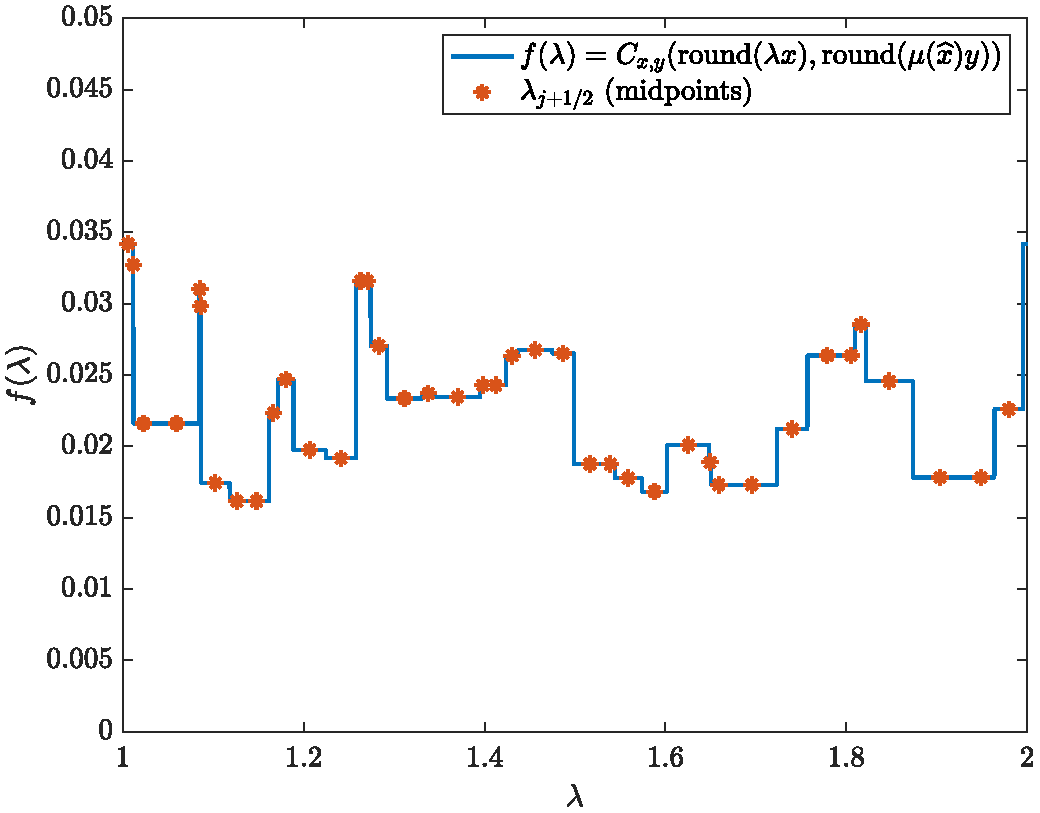
\includegraphics[width=0.4\textwidth]{figures/breakpoints_new.pdf}
\end{center}
\item Approximation of the optimum via (1D) derivative free optimization 
$$
\min_{\lambda\in\R} \norm{xy^T-\round(\lambda x)\round(\mu(\lambda) y)^T}
$$
\end{itemize}

\end{frame}

\begin{frame}{Application to butterfly quantization}
\begin{center}
  \only<1 >{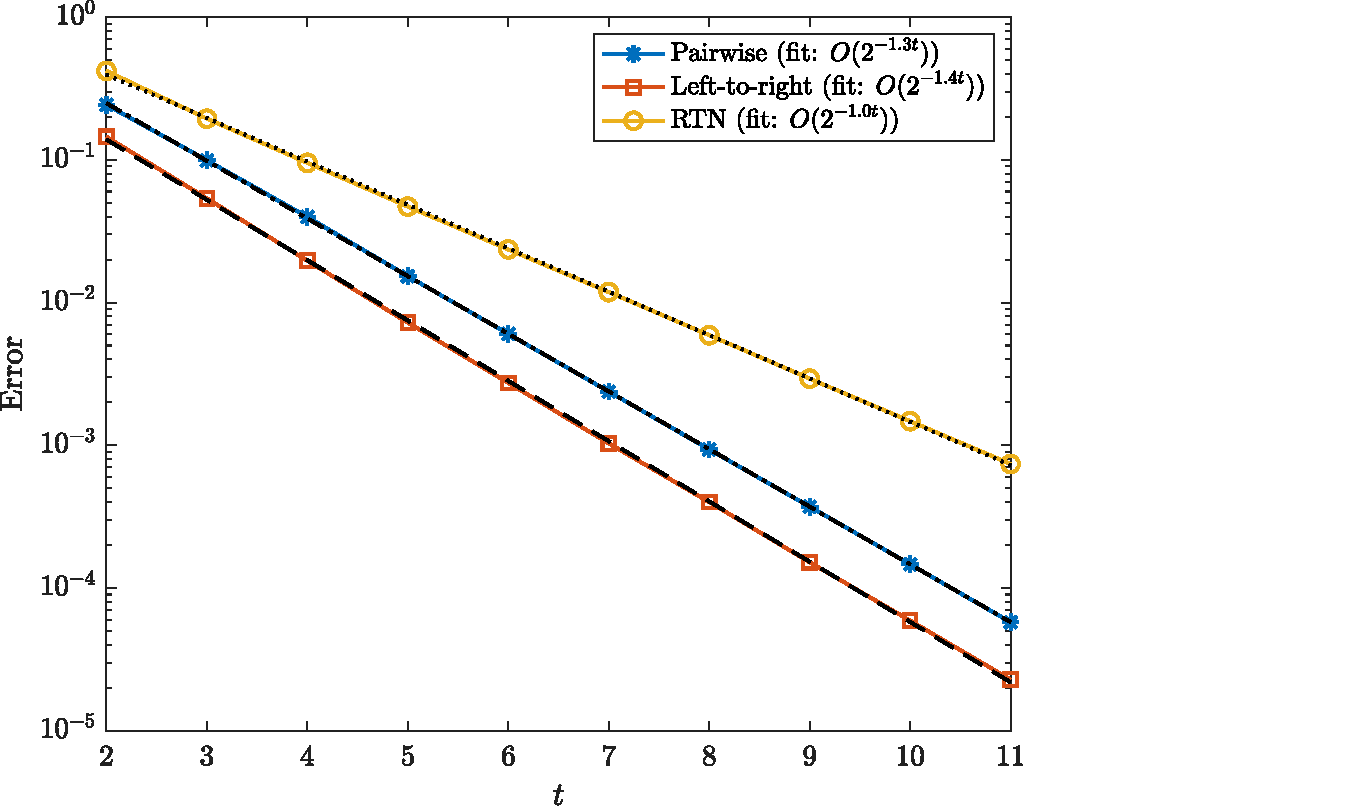
\includegraphics[width=0.7\textwidth]{figures/results_0}}%
  \only<2 >{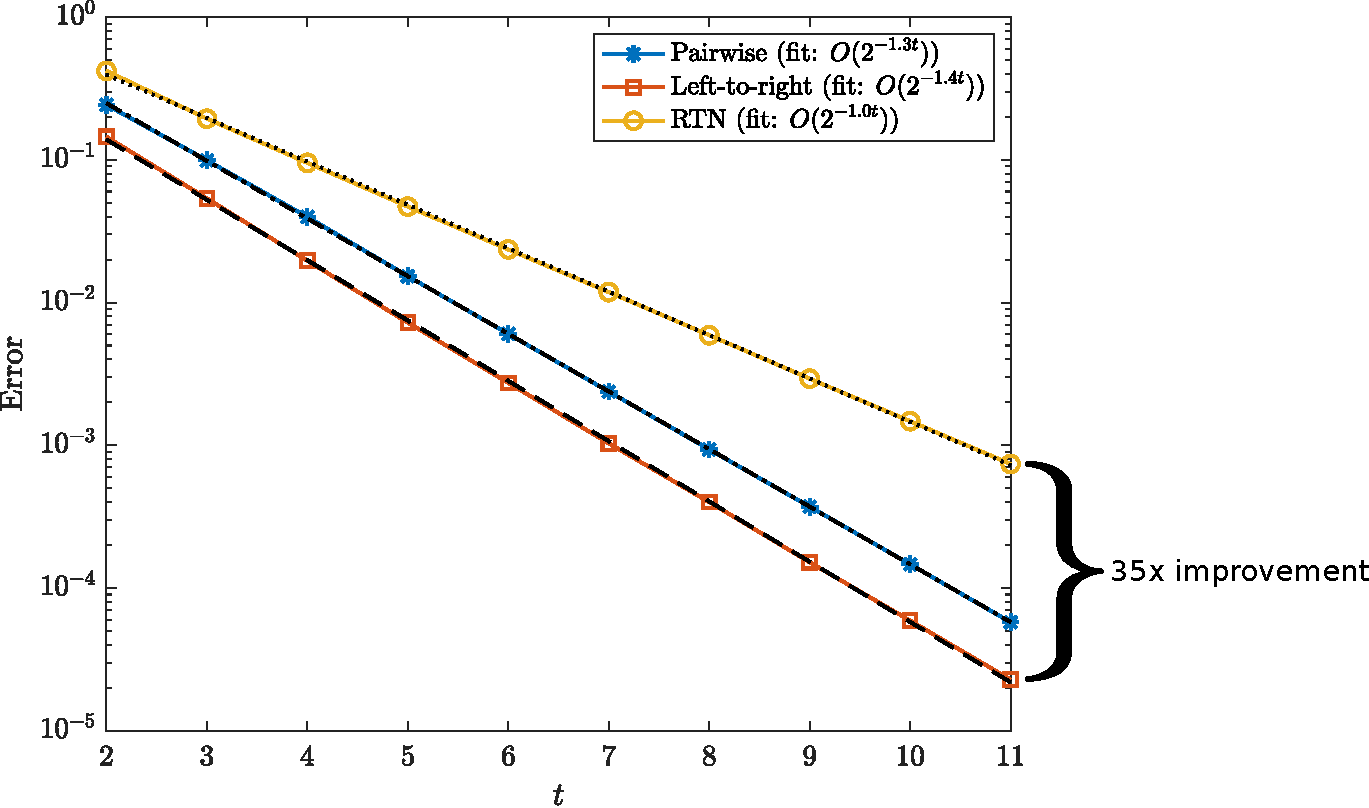
\includegraphics[width=0.7\textwidth]{figures/results_1}}%
  \only<3->{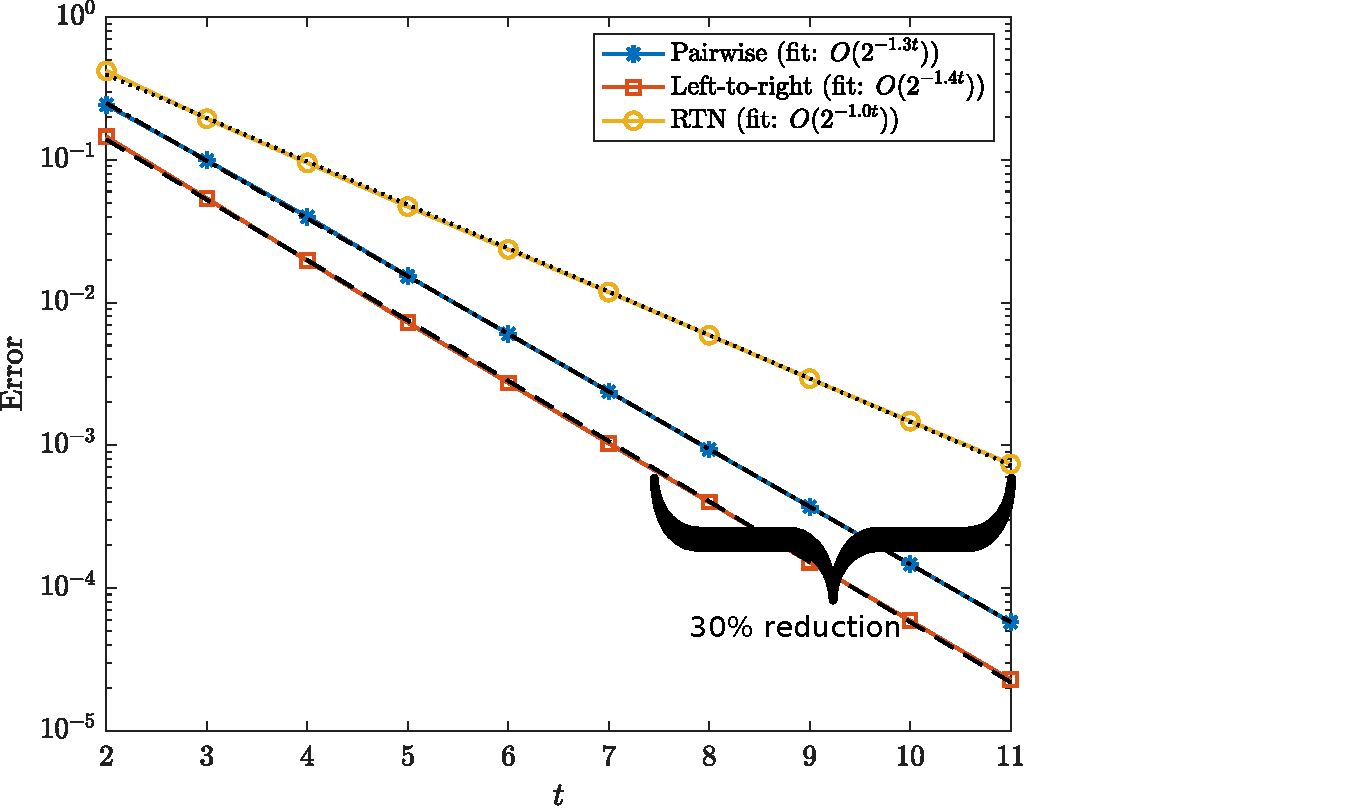
\includegraphics[width=0.7\textwidth]{figures/results_2}}%
\end{center}
\begin{itemize}
\item Randomly generated butterfly factors
\item<2-> Significant accuracy improvement\ldots
\item<3->\ldots or, equivalently, 
\alert{can reduce storage by about $30\%$ with no loss of accuracy}
\end{itemize}
\end{frame}

\end{comment}

	

	
		\part{Exploiting hierarchies of arithmetic precisions  }
	\frame[plain]{\partpage}

	
\begin{frame}{Floating-point arithmetic}

    
  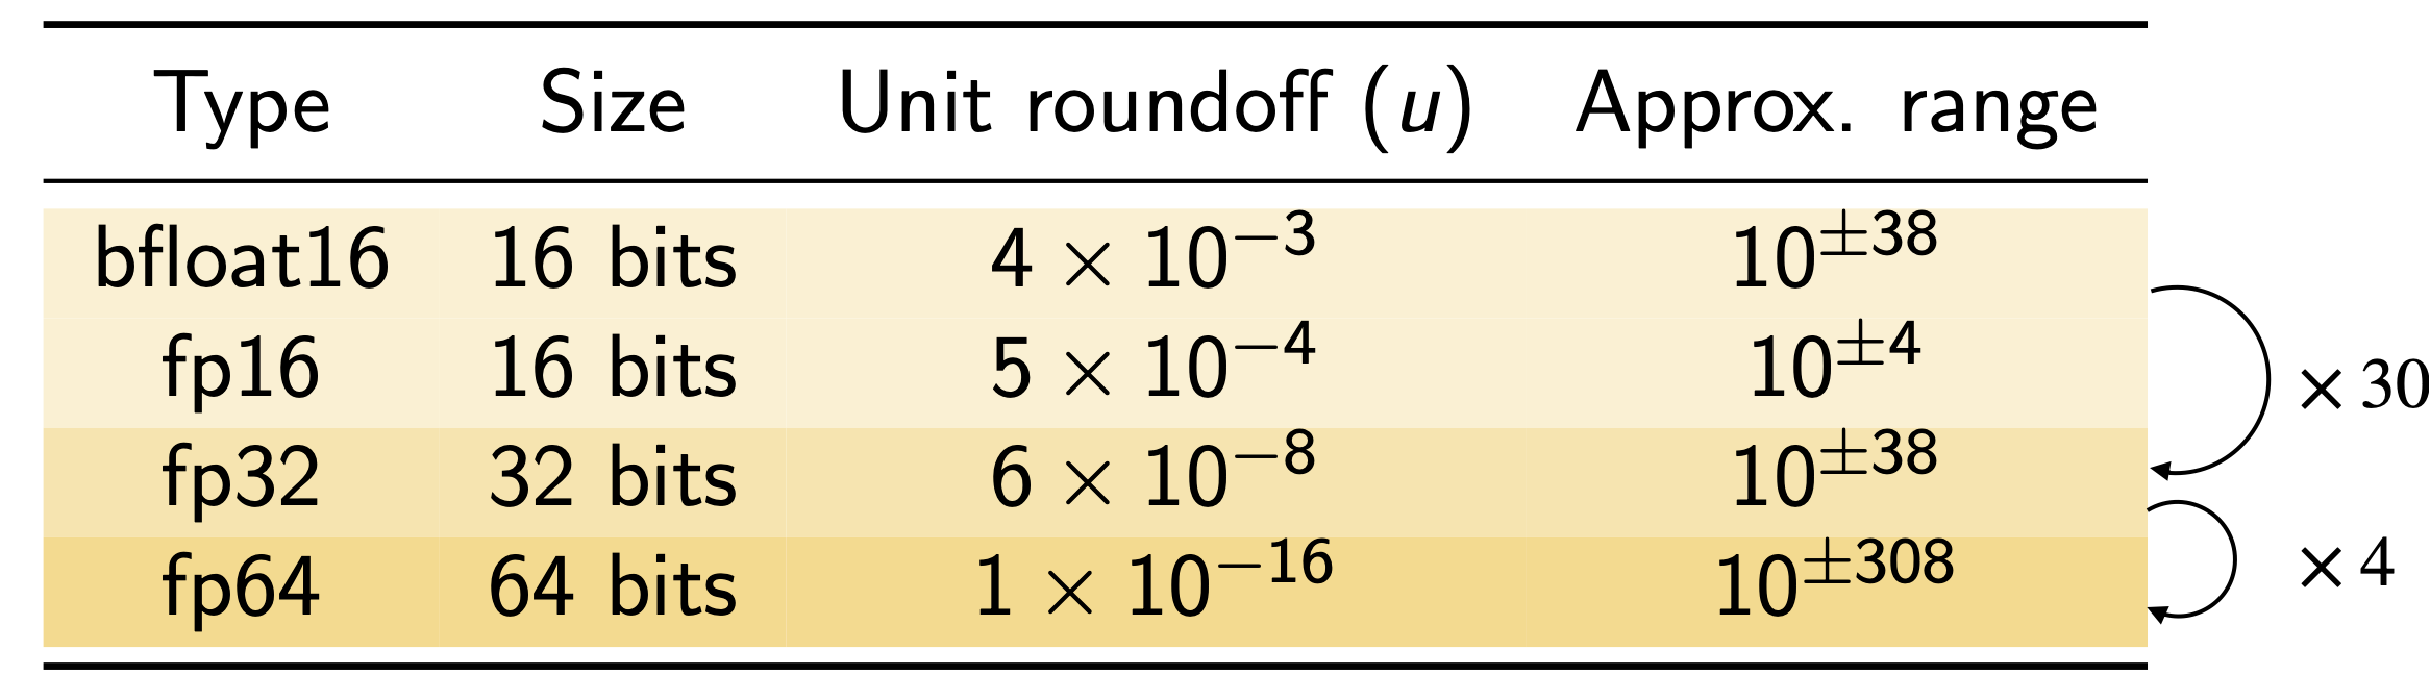
\includegraphics[width=\textwidth]{figures/table_precisions}

\vspace{0.6cm}

\begin{columns}
\begin{column}{0.5\textwidth}
  Low precisions 
  \begin{itemize}
   \item[\textcolor{green}{\faSmile}]  \alert{Reduction} of energy and increased speed 
     \item[\textcolor{red}{\faFrown}]      \alert{Loss} of accuracy
  \end{itemize}
  \end{column}
  \begin{column}{0.5\textwidth}
  $\rightarrow$ Mixed precision
  \begin{itemize}
  \item Forward pass of neural networks \footnotesize{ \textcolor{mygreen}{[El Arar, Filip, Mary, R., IMAJNA, 2026]}}
\item \alt<2->{\fbox{Newton's method}}{Newton's method}
 \end{itemize}
   \end{column}
    \end{columns}
\end{frame}




\begin{comment}
\begin{frame}{My contribution (I): mixed precision inference}
\begin{columns}
\begin{column}{0.5\textwidth}
\begin{center}
\includegraphics[width=\textwidth]{NN_paul_nofrecce.pdf}
\end{center}
\begin{itemize}
\item Forward pass of a network with $L$ layers:
\[
\alert{h_\ell = \phi_\ell(W_\ell h_{\ell-1})}, \quad \ell=1,\ldots,L
\]
where
\begin{itemize}
\item $W_\ell$: weight matrices
\item $\phi_\ell$: activation functions
\item $h_0 = x$: input 
\item $h_L$: output
\end{itemize}
\vspace{0.2cm}
\begin{center}
\includegraphics[width=0.45\textwidth]{layerl.pdf}
\end{center}
\end{itemize}
\end{column}
\begin{column}{0.5\textwidth}
\begin{itemize}
\item \alert{Quantization} stores the weights in reduced precision. 
\item \alert{Accumulation} ($W_\ell h_{\ell-1}$) is often kept in high precision
%\begin{itemize}
%\item Specialized hardware provides efficient high precision accumulators (e.g., NVIDIA tensor cores)
%\item Model accuracy is more sensitive to accumulation precision than storage precision 
%\end{itemize}
\item but 
can significantly improve performance, especially in \alert{resource-limited environments}
\end{itemize}

\end{column}
\end{columns}

\end{frame}






\begin{frame}{Error analysis of the forward pass}

\begin{columns}
\begin{column}{0.7\textwidth}
\begin{tcolorbox}
\begin{small}
The computed output $\hh_\ell$ of any layer $\ell$ satisfies
	\[
	\hh_\ell = h_\ell \circ (\mathbf{1}+\Delta h_\ell), \quad
	\abs{\Delta h_\ell} \le \eps_\ell^h,
	\]
	where $\eps_\ell^h$ satisfies the first-order recurrence
	\[
	\eps_\ell^h \approx \alert{\kappa_{\phi_\ell}}\circ\big(\eps_\ell^W + \norminf{ \eps_{\ell-1}^h}\big) + \eps_\ell^\phi.
	\]
	\end{small}
\end{tcolorbox}
\end{column}
\begin{column}{0.3\textwidth}
 After some simplifications
\begin{align*}
		\norminf{\eps_L^h}\propto \sum_{\ell=1}^L
		\norminf{\alert{\kappa_{\phi_\ell}}  \circ \eps_\ell^W}
\end{align*}
\end{column}
\end{columns}
\pause
\begin{itemize}
\item Large potential variations of condition numbers:

\begin{center}
  \includegraphics[width=0.3\textwidth]{cond_relu}%
  \includegraphics[width=0.3\textwidth]{cond_tanh}
\end{center}

\item[$\Raw$] 
%The components $(\eps_\ell^W)_i$ should be chosen to be \alert{inversely
%proportional} to $(\kappa_\ell)_i := (\kappa_{\phi_\ell}(v_\ell) \circ \kappa_{v_\ell})_i$ $\Raw$ 
mixed precision opportunity!
\end{itemize}

\end{frame}

\begin{frame}{Experimental results: ReLU}
%\begin{columns}
%\begin{column}{0.5\textwidth}
%\rho=
%\end{column}
%\begin{column}{0.5\textwidth}
\centering
\includegraphics[width=0.7\textwidth]{fmnist_mlp5_relu.pdf}
%\end{column}
%\end{columns}

\vspace{0.1cm}
\small{ \textcolor{mygreen}{[El Arar, Filip, Mary, R., IMAJNA, 2026]}}
\end{frame}

\end{comment}


\begin{frame}{Mixed precision Newton's methods}

\begin{tcolorbox}{Newton's method}
 % \begin{align*}
    %  &d_i:= -H(x_i)^{-1}g(x_i)\\
     % &x_{i+1}=x_i+d_i
  %\end{align*}
   \begin{enumerate}
   \item  Compute $g(x_i)$       
    \item  Solve $H(x_i)d_i = -g(x_i)$    
 \item  Update $x_{i+1} = x_i + d_i$ 
  \end{enumerate}
\end{tcolorbox}

\begin{tcolorbox}{Error model}
  \begin{align*}
      &\widehat{d}_i := - \big(H(\widehat{x}_i) + \textcolor{myblue}{E^H_i}\big)^{-1}\big(g(\widehat{x}_i) +\textcolor{red!70!black}{e^g_i}\big), \\
      &\widehat{x}_{i+1} =  \widehat{x}_i + \widehat{d}_i + \textcolor{myyel!70!black}{e^+_i}.
  \end{align*}
\end{tcolorbox}
      
      \pause
 
  \begin{tcolorbox}[
  title={Local convergence analysis},
      colback=white,
      colframe=gray!40,
      boxrule=0.4pt,
      arc=4pt,
      left=6pt, right=6pt, top=4pt, bottom=4pt,
    ]
  \begin{equation*}
      \norm{ \widehat{x}_{i+1} - x^*} \leq
     \alpha_i\norm{\widehat{x}_i - x^*}^2
      +\textcolor{myblue}{\beta_i}\norm{ \widehat{x}_i -x^* }
      +\textcolor{red!70!black}{\limacc},
    \end{equation*}
   
    \end{tcolorbox}
      \small{ \textcolor{mygreen}{[Carrino, Brisebarre, Mary, R., submitted to COAP, 2026]}}

    \end{frame}
    
    \begin{frame}{Floating point Newton's method}
   
   
  \begin{tcolorbox}[
      colback=white,
      colframe=gray!40,
      boxrule=0.4pt,
      arc=4pt,
      left=1pt, right=1pt, top=1pt, bottom=1pt,
    ]
  \begin{enumerate}
   \item  Compute $g(x_i)$        in \textcolor{gray!70!black}{$u_g$} \\
 \item  Solve $H(x_i)d_i \approx -g(x_i)$     in \textcolor{myblue!70!black}{$u_H$} \\
 \item  Update $x_{i+1} = x_i + d_i$  in \textcolor{myyel!70!black}{$u$} \\
  \end{enumerate}
  \end{tcolorbox}
  
  \begin{itemize}
  \item 
  The setting of interest is (precision $\propto 1/u$)
  \begin{equation*}
    \tikz[remember picture, baseline=(ug.base)]{\node[inner sep=1pt] (ug) {$u_g$};}
    \;\leq\;
    \tikz[remember picture, baseline=(u.base)]{\node[inner sep=1pt] (u) {$u$};}
    \;\leq\;
    \tikz[remember picture, baseline=(uH.base)]{\node[inner sep=1pt] (uH) {$u_H$};}
  \end{equation*}
  \pause
  
 \item Inexact Newton: 
            $
\norm{H(x_i)d_i+g(x_i)}\leq \eta \norm{g(x_i)}.
$

Error on the Hessian:
$
O( u_H) + O(\eta)
$
%where $\zeta_i = \norm{H(\widehat{x}_i)}\norm{\widehat{d}_i}/\norm{g(\widehat{x}_i)}$
\begin{center}
  %  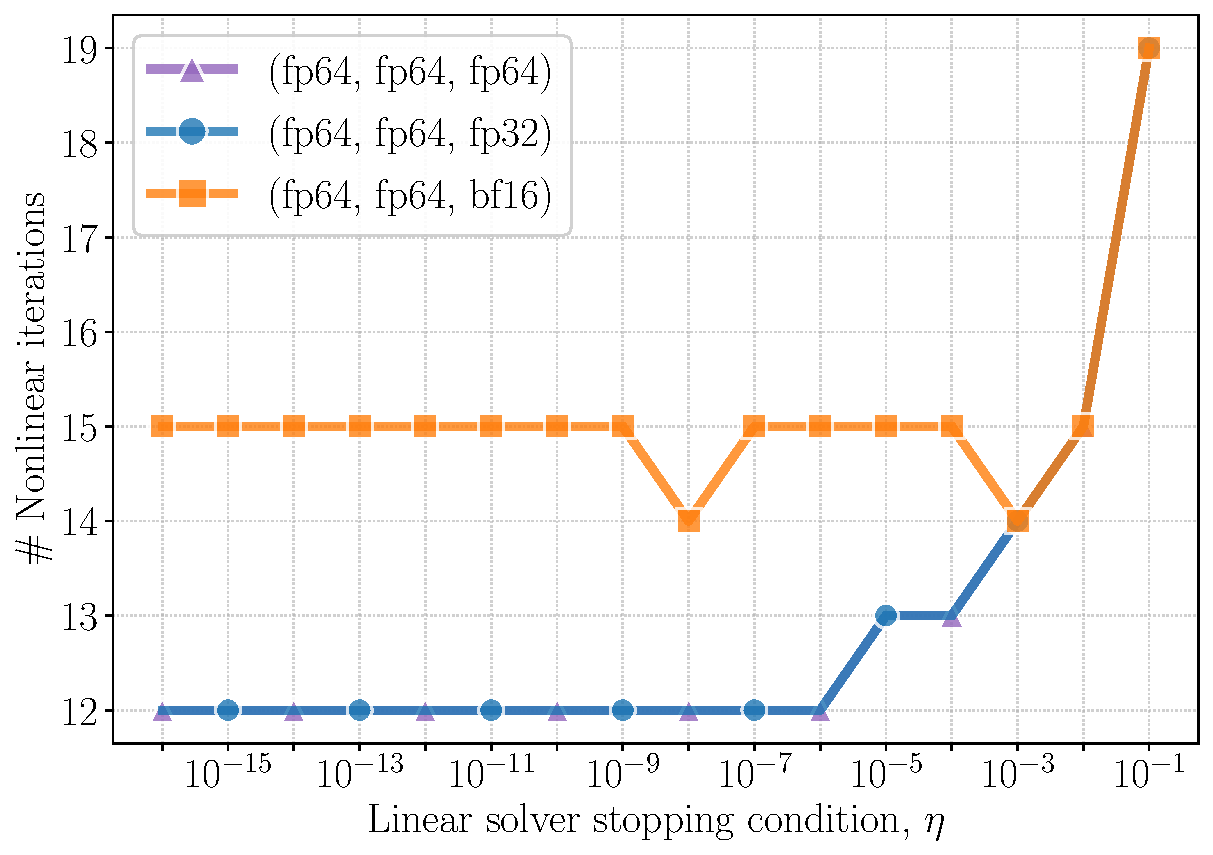
\includegraphics[width=.5\linewidth]{figures/Newton_MULTIPLE_ETA.pdf}
        \includegraphics[width=.5\linewidth]{figures/in_etas_2.png}

\end{center}
\end{itemize}
  
\end{frame}

\begin{comment}
\begin{frame}{Floating-point arithmetic Newton's method}
\begin{columns}
\begin{column}{0.5\textwidth}
\begin{tcolorbox}[
      colback=white,
      colframe=gray!40,
      boxrule=0.4pt,
      arc=4pt,
      left=1pt, right=1pt, top=1pt, bottom=1pt,
    ]
  \begin{enumerate}
   \item  Compute $g_i = g(x_i)$        in \textcolor{gray!70!black}{$u_g$} \\
 \item  Solve $H(x_i)d_i = -g_i$     in \textcolor{myblue!70!black}{$u_H$} \\
 \item  Update $x_{i+1} = x_i + d_i$  in \textcolor{myyel!70!black}{$u$} \\
  \end{enumerate}
  \end{tcolorbox}
  The setting of interest is
  \begin{equation*}
    \tikz[remember picture, baseline=(ug.base)]{\node[inner sep=1pt] (ug) {$u_g$};}
    \;\leq\;
    \tikz[remember picture, baseline=(u.base)]{\node[inner sep=1pt] (u) {$u$};}
    \;\leq\;
    \tikz[remember picture, baseline=(uH.base)]{\node[inner sep=1pt] (uH) {$u_H$};}
  \end{equation*}

  \begin{itemize}
    \item<2-> \textcolor{myyel!70!black}{\textbf{Target precision}}
        \item<3-> \textcolor{myblue!70!black}{\textbf{Reduced precision linear solver}} ($u_H$ large): reduced cost per iteration.
    \item<4-> \textcolor{gray!70!black}{\textbf{Accurate gradient}} ($u_g$ small): better limiting accuracy $\limacc$.
  \end{itemize}
  
  

  \begin{tikzpicture}[overlay, remember picture]
    \only<2->{
      \draw[rounded corners=3pt, thick, color=myyel!70!black, fill=myyel!10, fill opacity=0.3]
        ([xshift=-2pt, yshift=2pt]u.north west) rectangle
        ([xshift=2pt,  yshift=-2pt]u.south east);
    }
    \only<4->{
      \draw[rounded corners=3pt, thick, color=gray!70!black, fill=gray!10, fill opacity=0.3]
        ([xshift=-2pt, yshift=2pt]ug.north west) rectangle
        ([xshift=2pt,  yshift=-2pt]ug.south east);
    }
    \only<3->{
      \draw[rounded corners=3pt, thick, color=myblue!70!black, fill=myblue!10, fill opacity=0.3]
        ([xshift=-2pt, yshift=2pt]uH.north west) rectangle
        ([xshift=2pt,  yshift=-2pt]uH.south east);
    }
  \end{tikzpicture}
\end{column}

\begin{column}{0.5\textwidth}
    \begin{tcolorbox}[
    title=  Error model,
      colback=white,
      colframe=gray!40,
      boxrule=0.4pt,
      arc=4pt,
      left=1pt, right=1pt, top=1pt, bottom=1pt,
    ]
    \begin{tiny}
      \begin{align*}
        &\widehat{d}_i := - \big(H(\widehat{x}_i) + \tikz[remember picture, baseline=(EHm.base)]{\node[inner sep=1pt] (EHm) {$E^H_i$};}\big)^{-1}\big(g(\widehat{x}_i) + \tikz[remember picture, baseline=(Egm.base)]{\node[inner sep=1pt] (Egm) {$e^g_i$};}\big), \\
        &\widehat{x}_{i+1} =  \widehat{x}_i + \widehat{d}_i + \tikz[remember picture, baseline=(Epm.base)]{\node[inner sep=1pt] (Epm) {$e^+_i$};}.
      \end{align*}
      \end{tiny}
    \end{tcolorbox}
  \begin{itemize}
    \item<2-> \textcolor{myyel!70!black}{$\tikz[remember picture, baseline=(Ep2.base)]{\node[inner sep=1pt] (Ep2) {$\norm{e^+_i}$};}  \lesssim u$}
        \item<3-> \textcolor{myblue!70!black}{$\tikz[remember picture, baseline=(EH2.base)]{\node[inner sep=1pt] (EH2) {$\norm{E^H_i}$};} \approx O(u_H)$}, if linear system is solved with a backward stable method can take into account \alert{quasi-Newton} and \alert{inexact Newton} errors;
    \item<4-> \textcolor{gray!70!black}{$\tikz[remember picture, baseline=(Eg2.base)]{\node[inner sep=1pt] (Eg2) {$\norm{e^g_i}$};} \approx O(u_g)$}.
  \end{itemize}

  \begin{tikzpicture}[overlay, remember picture]
    \only<2->{
      \draw[rounded corners=3pt, thick, color=myyel!70!black, fill=orange!10, fill opacity=0.3]
        ([xshift=-2pt, yshift=2pt]Ep2.north west) rectangle
        ([xshift=2pt,  yshift=-2pt]Ep2.south east);
      \draw[rounded corners=3pt, thick, color=myyel!70!black, fill=myyel!10, fill opacity=0.3]
        ([xshift=-2pt, yshift=2pt]Epm.north west) rectangle
        ([xshift=2pt,  yshift=-2pt]Epm.south east);
    }
    \only<3->{
      \draw[rounded corners=3pt, thick, color=myblue!70!black, fill=myblue!10, fill opacity=0.3]
        ([xshift=-2pt, yshift=2pt]EH2.north west) rectangle
        ([xshift=2pt,  yshift=-2pt]EH2.south east);
      \draw[rounded corners=3pt, thick, color=myblue!70!black, fill=myblue!10, fill opacity=0.3]
        ([xshift=-2pt, yshift=2pt]EHm.north west) rectangle
        ([xshift=2pt,  yshift=-2pt]EHm.south east);
    }
    \only<4->{
      \draw[rounded corners=3pt, thick, color=gray!70!black, fill=gray!10, fill opacity=0.3]
        ([xshift=-2pt, yshift=2pt]Eg2.north west) rectangle
        ([xshift=2pt,  yshift=-2pt]Eg2.south east);
      \draw[rounded corners=3pt, thick, color=gray!70!black, fill=gray!10, fill opacity=0.3]
        ([xshift=-2pt, yshift=2pt]Egm.north west) rectangle
        ([xshift=2pt,  yshift=-2pt]Egm.south east);
    }
  \end{tikzpicture}
  \end{column}

  \end{columns}
  \begin{tcolorbox}[
      colback=white,
      colframe=gray!40,
      boxrule=0.4pt,
      arc=4pt,
      left=1pt, right=1pt, top=1pt, bottom=1pt,
    ]
  \begin{enumerate}
   \item  Compute $g_i = g(x_i)$        in \textcolor{gray!70!black}{$u_g$} \\
 \item  Solve $H(x_i)d_i = -g_i$     in \textcolor{myblue!70!black}{$u_H$} \\
 \item  Update $x_{i+1} = x_i + d_i$  in \textcolor{myyel!70!black}{$u$} \\
  \end{enumerate}
  \end{tcolorbox}
  The setting of interest is
  \begin{equation*}
    \tikz[remember picture, baseline=(ug.base)]{\node[inner sep=1pt] (ug) {$u_g$};}
    \;\leq\;
    \tikz[remember picture, baseline=(u.base)]{\node[inner sep=1pt] (u) {$u$};}
    \;\leq\;
    \tikz[remember picture, baseline=(uH.base)]{\node[inner sep=1pt] (uH) {$u_H$};}
  \end{equation*}
\end{frame}
\end{comment}

\begin{comment}
\begin{frame}{Floating-point arithmetic Newton's method}

\begin{tcolorbox}[
      colback=white,
      colframe=gray!40,
      boxrule=0.4pt,
      arc=4pt,
      left=1pt, right=1pt, top=1pt, bottom=1pt,
    ]
  \begin{enumerate}
   \item  Compute $g_i = g(x_i)$        in \textcolor{gray!70!black}{$u_g$} \\
 \item  Solve $H(x_i)d_i = -g_i$     in \textcolor{myblue!70!black}{$u_H$} \\
 \item  Update $x_{i+1} = x_i + d_i$  in \textcolor{myyel!70!black}{$u$} \\
  \end{enumerate}
  \end{tcolorbox}
  The setting of interest is
  \begin{equation*}
    \tikz[remember picture, baseline=(ug.base)]{\node[inner sep=1pt] (ug) {$u_g$};}
    \;\leq\;
    \tikz[remember picture, baseline=(u.base)]{\node[inner sep=1pt] (u) {$u$};}
    \;\leq\;
    \tikz[remember picture, baseline=(uH.base)]{\node[inner sep=1pt] (uH) {$u_H$};}
  \end{equation*}

  \begin{itemize}
    \item<2-> \textcolor{myyel!70!black}{\textbf{Target precision}}
        \item<3-> \textcolor{myblue!70!black}{\textbf{Reduced precision linear solver}} ($u_H$ large): reduced cost per iteration.
    \item<4-> \textcolor{gray!70!black}{\textbf{Accurate gradient}} ($u_g$ small): better limiting accuracy $\limacc$.
  \end{itemize}
  
  

  \begin{tikzpicture}[overlay, remember picture]
    \only<2->{
      \draw[rounded corners=3pt, thick, color=myyel!70!black, fill=myyel!10, fill opacity=0.3]
        ([xshift=-2pt, yshift=2pt]u.north west) rectangle
        ([xshift=2pt,  yshift=-2pt]u.south east);
    }
    \only<4->{
      \draw[rounded corners=3pt, thick, color=gray!70!black, fill=gray!10, fill opacity=0.3]
        ([xshift=-2pt, yshift=2pt]ug.north west) rectangle
        ([xshift=2pt,  yshift=-2pt]ug.south east);
    }
    \only<3->{
      \draw[rounded corners=3pt, thick, color=myblue!70!black, fill=myblue!10, fill opacity=0.3]
        ([xshift=-2pt, yshift=2pt]uH.north west) rectangle
        ([xshift=2pt,  yshift=-2pt]uH.south east);
    }
  \end{tikzpicture}

\end{frame}
\end{comment}

\begin{comment}
\begin{frame}{Numerical results: mixed precision Newton}
    \begin{center}
Precision sets: $(u_g, u, u_H)$
   
 \only<1>{   \includegraphics[width=0.55\linewidth]{figures/exp1.pdf}}
     \only<2>{     \includegraphics[width=0.55\linewidth]{figures/exp2.pdf}}

  \end{center}
  \vfill
  
\end{frame}
\end{comment}





\begin{frame}[plain]
    \centering
    \vfill
    {\usebeamerfont{part title}\usebeamercolor[fg]{part title}\Huge Conclusion\par}
    \vfill
\end{frame}

\begin{frame}{Other important topics}
\begin{itemize}
\item \alert{Rescaling invariant} quantization and neural networks representations \small{ \textcolor{mygreen}{ [Gribonval, Mary, R., SISC, 2026], [Chaumette, Gribonval, R., submitted, 2026], [Gonon, Brisebarre, R., Gribonval, ICLR 2024 and ICML 2025]}}
\item Link between \alert{BCD and multiresolution methods} \small{ \textcolor{mygreen}{[Lauga, Riccietti, Briceño-Arias, Pustelnik, Gonçalves, 2025], [Desainte-Maréville, Foare, Gonçalves, Pustelnik, R., Eusipco, 2026]}}
\item Multilevel \alert{Plug and Play}  \small{ \textcolor{mygreen}{[Laurent, Tachella, R., Pustelnik, TCI, 2025]}}
\item \alert{Sparse neural networks} \small{ \textcolor{mygreen}{[Le, R., Gribonval, NeurIPS, 2023], [Gribonval, R., Le, Zheng, IEEE SPM, 2025]}}
\end{itemize}
\end{frame}



\begin{frame}{Take-aways}
\begin{itemize}
\item Structured
hierarchies constitute a \alert{powerful and versatile paradigm}
\item Important to \alert{leverage} structure when present to \alert{improve accuracy or accelerate convergence}
\item Structure provides \alert{unifying lens} through which seemingly different problems can be approached with common tools
\item Leveraging structure in practice is \alert{challenging} ! 
\end{itemize}
\end{frame}


	
\begin{frame}{Some perspectives }
    \includegraphics[width=\linewidth]{figures/perspectives4.pdf}

\end{frame}	
		
		

         


\begin{frame}[t]
\frametitle{Team work!}
\vfill
%[trim={left bottom right top},clip]
\begin{center}
\begin{tabular}{ccc}
\includegraphics[trim={9cm 0cm  9cm 0cm},clip, height=2.5cm]{photos/giuseppe.jpeg}&
\includegraphics[trim={9cm 0cm  9cm 0cm},clip, height=2.5cm]{photos/edgar.jpeg}&
\includegraphics[trim={9cm 0cm  9cm 0cm},clip, height=2.5cm]{photos/mael.jpeg}\\
\includegraphics[trim={0cm 0cm  0cm 0cm},clip, height=2.5cm]{photos/filippo.jpeg}&
\includegraphics[trim={0cm 0cm  0cm 0cm},clip, height=2.5cm]{photos/valentin.png}&
\includegraphics[trim={20cm 0cm  20cm 0cm},clip, height=2.5cm]{photos/tung2.jpeg}\\
\includegraphics[trim={9cm 0cm  9cm 0cm},clip, height=2.5cm]{photos/leon.jpeg}&
\includegraphics[trim={0cm 0 0cm 0cm},clip, height=2.5cm]{photos/antoine.jpeg}&
\includegraphics[trim={0 0  0cm 0cm},clip, height=2.5cm]{photos/lauga.jpg}
\end{tabular}
\end{center}
\end{frame}


\begin{frame}{STOP workshop}
\begin{center}
\includegraphics[scale=0.3]{../../loghi_firme/ENS_foto.jpeg}\\
\alert{ST}ructured \alert{OP}timization for inverse and learning problems\\
29 september - 01 october 2026\\
ENS Lyon, site monod\\
\url{https://stop.sciencesconf.org}\\
Starts tomorrow \alert{8:50} in \alert{Amphi B}, third floor  
\end{center}
\vspace{0.5cm}
 %\pause
 \begin{center}
    \alert{\Large{ \textit{Thank you for your attention!}}}
\end{center} 
\end{frame}

\appendix
\begin{frame}{Numerical results - Finite sum minimization}

\begin{figure}[h!]
    \centering
    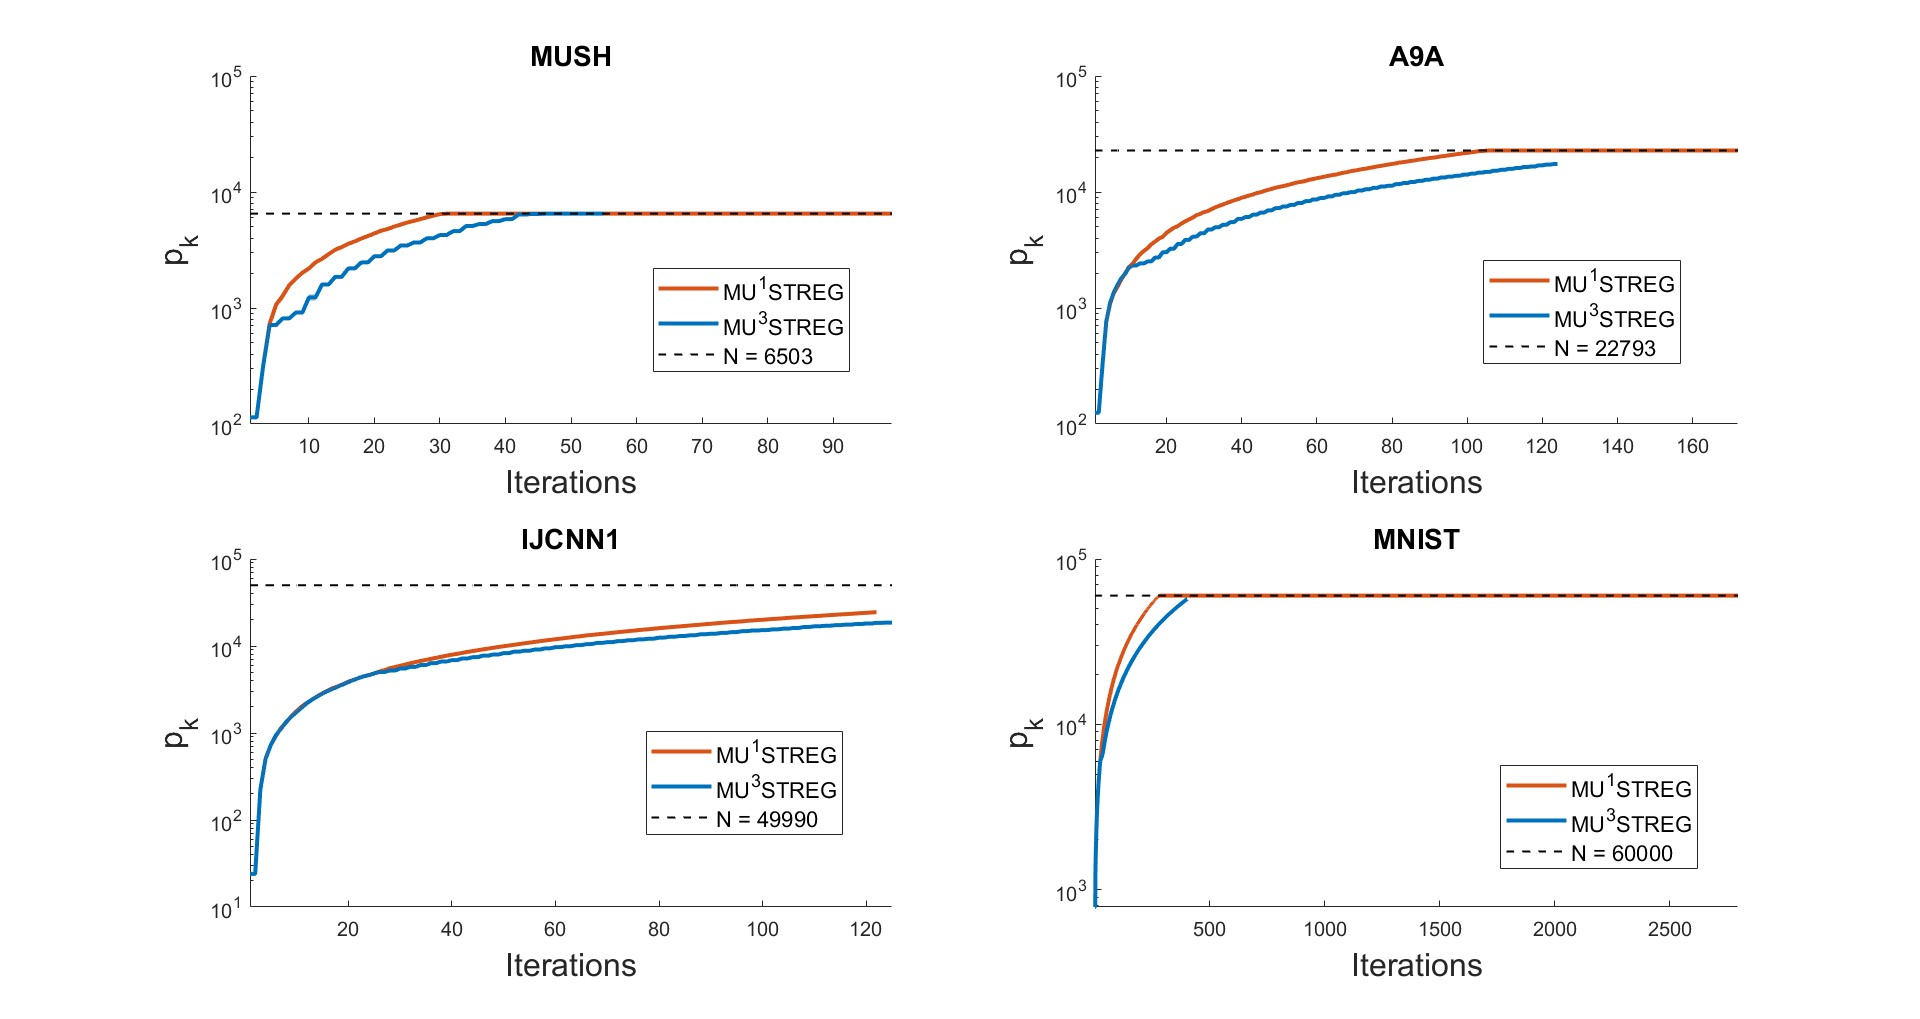
\includegraphics[width=\linewidth]{figures/LEAST-SQUARES_p_k_vs_ev_SHADED.jpg}
    \caption{Cardinality of the sample set at the finest level and the full size $N$ along the iterations. $\lvert\mathcal{S}_k^{\ell_{\max}}\rvert=p_k:=\min\{N,\max\{100k+n+2, \alert{\lambda_k^2\}}\}$ }
    \label{fig: pk vs. ev.}
\end{figure}
	\end{frame}


%\begin{frame}{SVRG update}
%$$x_{k+1}=x_k-\alert{\alpha}\quadre{\frac{1}{b}\sum_{i_k\in I_k}\nabla f^{i_k}(x_k) +\textcolor{blue}{ \tonde{\nabla f(\tilde{x}_0)-\frac{1}{b}\sum_{i_k\in I_k}\nabla f^{i_k}(\tilde{x}_0)}}},$$ 
%where $\tilde{x}_0$ is updated every $m$ iterations, when the full gradient is re-evaluated. 
%\end{frame}

\begin{frame}{The theory - assumptions}
Let $\mathcal{F}^{M\, F}_{k-1/2}$ be
 the $\sigma$-algebra generated by $M_0,\dots,M_{k}$
and $F_0,\dots,F_{k-1}$ and  $\mathcal{F}^{M\, F}_{k-1}$ be
 the $\sigma$-algebra generated by $M_0,\dots,M_{k-1}$
and $F_0,\dots,F_{k-1}$.


\begin{itemize}
\item 
	 $f:\mathbb{R}^n\rightarrow\mathbb{R}$ and $\coarse_k:\mathbb{R}^{n_c}\rightarrow\mathbb{R}$ with $n\geq n_c$ have Lipschitz continuous gradients 

  %  In the setting of finite sum minimization, cf. Example 1, the assumption is satisfied if all the $f^{(i)}$ are smooth, which is quite a common assumption in this context \cite{garrigos2023handbook}. 
  \item $M_k$ \alert{$\alpha$-probabilistically $\kappa$-fully linear models}: $
\mathbb{P}(I_k|\mathcal{F}^{M\, F}_{k-1}) \geq \alpha,
$ $
I_k = \{M_k \text{ is a } \kappa\text{ -fully linear model of } f \text{ around } X_k\} 
$
\item $F_k$ \alert{$\beta$-probabilistically $\epsilon_f$-accurate estimates}: $\mathbb{P}(J_k|\mathcal{F}^{M\, F}_{k-1/2}) \geq \beta$, 
$
J_k = \{F_k,F_k^s \text{ are } \epsilon_f\text{-accurate estimates of } f(x_k) \text{ and } f(x_k+s_k), \text{ respectively, around } X_k\} 
$ $$
  \lvert f_k-f(x_k)\rvert\leq \frac{\epsilon_f}{\lambda_k^2} \text{ and } \lvert f_k^s-f(x_k+s_k)\rvert\leq \frac{\epsilon_f}{\lambda_k^2}.
  $$
  


\end{itemize}

		\end{frame}


\begin{frame}{Convergence theory: definitions}
\begin{block}{Definition 1}
Suppose that $\nabla f$ is Lipschitz continuous. Given $\lambda_k>0$, a function $m$ is a \textcolor{red}{$\kappa$-fully linear model} of $f$ around the iterate $x_k$ provided for $\kappa = (\kappa_f , \kappa_g)$, that for all $y$ in a neighborhood of $x_k$:
\begin{align*}
\|\nabla_x f (y) - \nabla_x m(y)\|\leq \frac{\kappa_g}{\lambda_k}, \\
|f (y) - m(y)| \leq \frac{\kappa_f}{\lambda_k^2}.
\end{align*}    
\end{block}   
\begin{block}{Definition 2}
A sequence of random models $\{M_k\}$ is said to be \textcolor{red}{$\alpha$-probabilistically $\kappa$-fully linear} with respect to the corresponding sequence $\{X_k,\Lambda_k\}$ 
if the events
$$
I_k = \{M_k \text{ is a } \kappa\text{ -fully linear model of } f \text{ around } X_k\} 
$$
satisfy the condition
$$
\mathbb{P}(I_k|\mathcal{F}^{M\cdot F}_{k-1}) \geq \alpha.
$$
where $\mathcal{F}^{M\, F}_{k-1}$
is the $\sigma$-algebra generated by $M_0,\dots,M_{k-1}$
and $F_0,\dots,F_{k-1}$
\end{block}
\end{frame}
\begin{frame}{Convergence theory: definitions}
\begin{block}{Definition 3}
The estimates $f_k$ and $f_k^s$ are said to be \textcolor{red}{$\epsilon_f$-accurate} estimates of $f(x_k)$ and $f(x_k+s_k)$ respectively, for a given $\lambda_k$ if 
  $$
  \lvert f_k-f(x_k)\rvert\leq \frac{\epsilon_f}{\lambda_k^2} \text{ and } \lvert f_k^s-f(x_k+s_k)\rvert\leq \frac{\epsilon_f}{\lambda_k^2}.
  $$
    
\end{block}
\begin{block}{Definition 4}
A sequence of random estimates $\{F_k,F_k^s\}$ is said to be \textcolor{red}{$\beta$-probabilistically $\epsilon_f$-accurate} with respect to the corresponding sequence $\{X_k,\Lambda_k,S_k\}$
if the events
\begin{align*}
J_k =& \{F_k,F_k^s \text{ are } \epsilon_f\text{-accurate estimates of } f(x_k) \\
& \text{ and } f(x_k+s_k), \text{ respectively, around } X_k\}
\end{align*}
 

satisfy the condition
$$
\mathbb{P}(J_k|\mathcal{F}^{M\cdot F}_{k-1/2}) \geq \beta,
$$
where $\epsilon_f$ is a fixed constant.    
\end{block}
    
\end{frame}




\begin{frame}{Data sets}
    The data sets are divided into a training set and a testing set as specified in Table below.
\begin{table}[h!]
    \centering
    \begin{tabular}{llll}
    Data set        & nr. of features ($n$)   & Training set size ($N$)& Testing set size ($N_t$) \\ \hline
    MNIST  & 784                     & 60000                  & 10000 \\
MUSH  & 112                     & 6503                   & 1621\\
    A9A    & 123                     & 22793                  & 9768\\
    IJCNN1 & 22                      & 49990                  & 91701\\
    \end{tabular}
    \caption{Data sets with number of features $n$ and number of instances of the training set $N$ and the testing set $N_t$.}
    \label{tab: datasets}
\end{table}
\end{frame}



%%%%% PINNs
\begin{frame}{Numerical results: MSE vs iterations}

{\bf Problem:} Heat equation
\begin{columns}
\begin{column}{0.4\textwidth}
\begin{equation*}
\begin{tiny}
  \left\{
  \begin{aligned}
      &\frac{\partial u(z,t)}{\partial t} = \frac{1}{(\alert{\omega}\pi)^2}\frac{\partial^2 u(z,t)}{\partial z^2},\\   
      &u(z,0)= \sin(\alert{\omega}\pi z), \;z \in [0,1], \\
      &u(0,t)= u(1,t)= 0, \;t \in [0,1],\\
  \end{aligned}
  \right.
  \end{tiny}
\end{equation*}

\end{column}
\begin{column}{0.6\textwidth}
\begin{figure}
\includegraphics[width=\linewidth]{images/heat_graph}
\end{figure}
\end{column}
    \end{columns}


    


\end{frame}



%%%%% STOCH 


		\begin{frame}{Proposed stochastic multilevel method (2 levels)}
	Mu$^\ell$STREG: First order \alert{adaptive regularization method}
	$$m_k(x_k+s)=\varphi_k(s)+\frac{\lambda_k\|g_k\|}{2}\|s\|^2$$
	\begin{itemize}
	\item  Fine level: $$\varphi_k(s)=f_k+g_k^Ts \quad \alert{f_k\approx f(x_k), \; g_k\approx \nabla f(x_k)}$$ 
	\item Coarse level: 
	\begin{subequations}\label{reg_taylor_model}
$$
\varphi_k(s)=  \coarse_k(\alert{R}x_k+s)+\underbrace{(R\gk-\nabla\coarse_k(Rx_k))^Ts}_{\text{first-order \,coherence}}
$$
    \end{subequations}
    \end{itemize}
	\end{frame}
	
	


	\begin{frame}{The theory - what are we interested in? }
	\begin{center}
	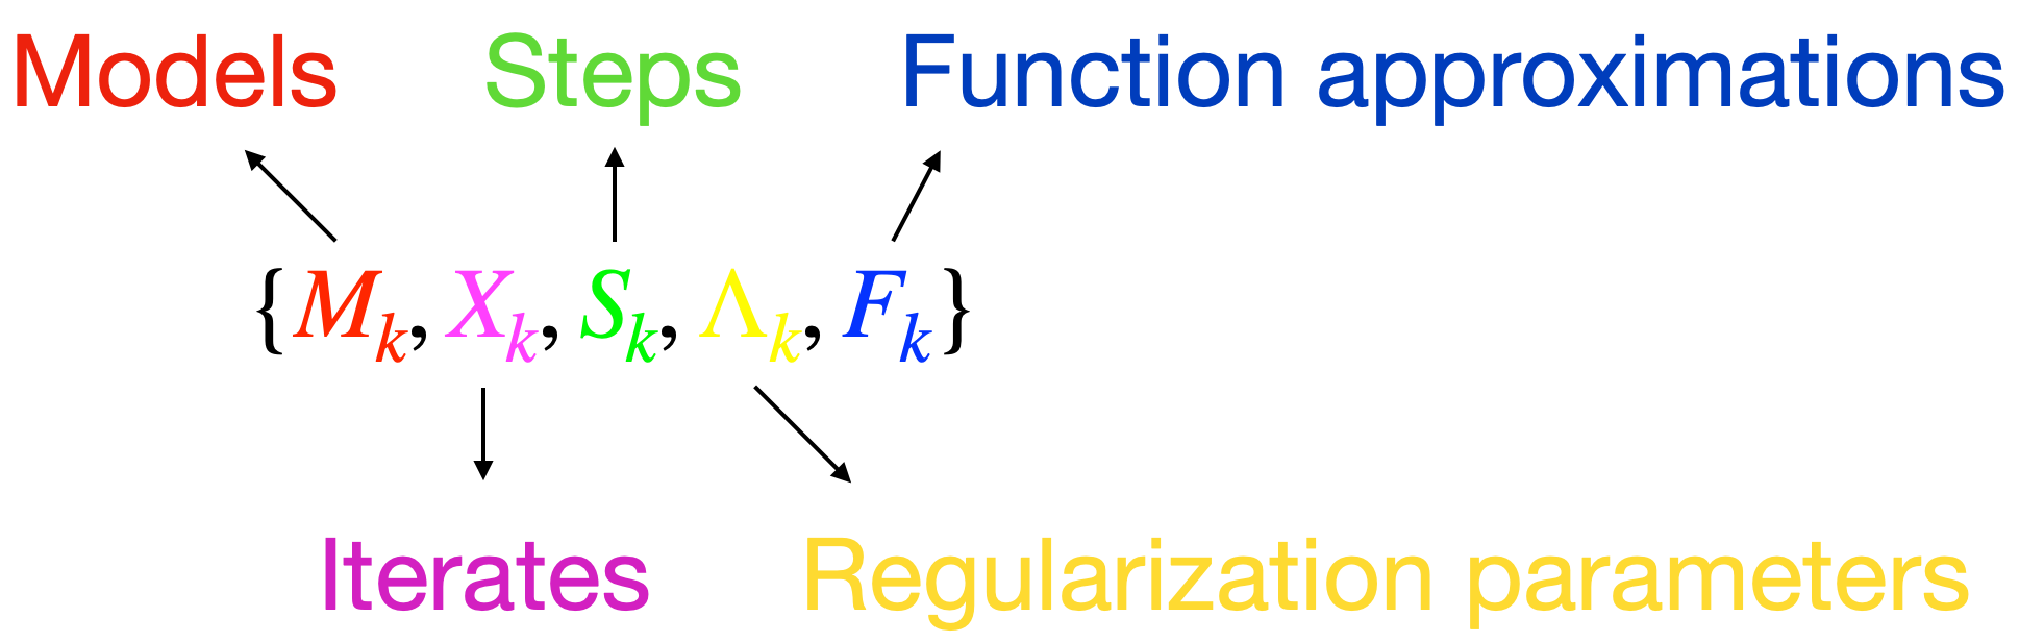
\includegraphics[scale=0.2]{figures/process}
	\end{center}
	\vspace{0.5cm}
	The stochastic process $\{M_k, X_k, S_k, \Lambda_k, F_k\}$, under certain conditions
on the sequences $\{M_k\}$ and $\{F_k\}$
 has desirable convergence
properties with \alert{probability one}. 

	\end{frame}
\begin{frame}{The theory - assumptions [simplified]}



\begin{itemize}
\item 
	 $f:\mathbb{R}^n\rightarrow\mathbb{R}$ and $\coarse_k:\mathbb{R}^{n_c}\rightarrow\mathbb{R}$ with $n\geq n_c$ have Lipschitz continuous gradients 

  %  In the setting of finite sum minimization, cf. Example 1, the assumption is satisfied if all the $f^{(i)}$ are smooth, which is quite a common assumption in this context \cite{garrigos2023handbook}. 
  \item The model $M_k$  to be \alert{$\kappa$-fully linear} around $X_k$ with probability $\alpha$  (\underline{only at fine level!}) 

\item The function approximations $F_k$ to be \alert{sufficiently accurate} ($\epsilon_f$) with probability $\beta$ 
  


\end{itemize}

		\end{frame}
	
	

	
	
		
	

	
\begin{frame}{The theory - results}
  Under suitable choices for           $\epsilon_f$,
     $\alpha$ and $\beta$ can be chosen so that, if the assumptions hold for these values, then the sequence of regularization parameters $\{\Lambda_k\}$ satisfies
     $$
\sum_{k=0}^{\infty}\frac{1}{\Lambda_k^2}<\infty
     $$
     and the sequence of iterates  $\{X_k\}$ satisfy
$$
\lim_{k\rightarrow\infty}\|\nabla_x f(X_k)\|=0
$$
     almost surely.
\end{frame}

\begin{frame}{Numerical results - Finite sum minimization}
\begin{block}{The problem}
\begin{equation*}
    \min_{x \in  \mathbb{R}^n}  F(x) =  \frac{1}{2N}\sum_{i=1}^N (y_i - \frac{1}{1 + \text{exp}(-y_ix^Tz_i)})^2,
\end{equation*}
with $(z_i,y_i)\in \mathbb{R}^n \times \{0,1\}$, for every $i=1,\dots,N$. 
\end{block}
\vspace{0.3cm}
\begin{block}{The methods}
\begin{itemize}
\item MU$^1$STREG: one level ($\approx$ STORM [Chen, et all. 2018])
\item MU$^3$STREG: three levels
\item Adagrad [J. Duchi, E. Hazan, and Y. Singer. (2011)]
\item SVRG [R. Johnson and T. Zhang. (2013)]
\end{itemize}
$$x_{k+1}=x_k-\alpha\left[\frac{1}{b}\sum_{i_k\in I_k}\nabla f^{i_k}(x_k) +\textcolor{blue}{ \left(\nabla f(\tilde{x}_0)-\frac{1}{b}\sum_{i_k\in I_k}\nabla f^{i_k}(\tilde{x}_0)\right)}\right],$$ 
where $\tilde{x}_0$ is updated every $m$ iterations 
\end{block}
	\end{frame}


	\begin{frame}{Results: comparison against  MU$^1$STREG{} and SVRG}
	 \begin{table}[h!]
\centering
\tiny
\begin{tabular}{|lccc|}
\hline
\multicolumn{4}{|c|}{MUSH}\\  
\hline
 & \multicolumn{1}{|c|}{SVRG }                   & \multicolumn{1}{c|}{MU$^1$STREG} & MU$^3$STREG \\\hline
\rowcolor{yellow}
\multicolumn{1}{|l|}{\textbf{Avg. \%tA}}               & \multicolumn{1}{c|}{98.69}                                                   & \multicolumn{1}{c|}{97.68}                                                    & 97.74                                                    \\
\multicolumn{1}{|l|}{\textbf{StD \%tA}}                & \multicolumn{1}{c|}{0.25}                                                         & \multicolumn{1}{c|}{0.50}                                                     & 0.48                                                     \\
\rowcolor{lightgray}
\multicolumn{1}{|l|}{\textbf{Avg. \#f/g}}              & \multicolumn{1}{c|}{341.89}                                                         & \multicolumn{1}{c|}{216.78}                                                   & 35.48                                                    \\

\multicolumn{1}{|l|}{\textbf{StD \#f/g}}               & \multicolumn{1}{c|}{722.65}                                                  & \multicolumn{1}{c|}{30.69}                                                    & 9.95                                                     \\ \hline
\multicolumn{4}{|c|}{A9A}                                                                                                                                                                                                                                                                                     \\ \hline
 & \multicolumn{1}{|c|}{SVRG }                   & \multicolumn{1}{c|}{MU$^1$STREG} & MU$^3$STREG \\\hline
\rowcolor{yellow}
\multicolumn{1}{|l|}{\textbf{Avg. \%tA}}               & \multicolumn{1}{c|}{85.00}                                                       & \multicolumn{1}{c|}{84.65}                                                    & 84.83                                                    \\
\multicolumn{1}{|l|}{\textbf{StD \%tA}}                & \multicolumn{1}{c|}{0.05}                                                          & \multicolumn{1}{c|}{0.04}                                                     & 0.07                                                     \\
\rowcolor{lightgray}
\multicolumn{1}{|l|}{\textbf{Avg. \#f/g}}              & \multicolumn{1}{c|}{840.77}                                                & \multicolumn{1}{c|}{207.68}                                                   & 90.87                                                    \\
\multicolumn{1}{|l|}{\textbf{StD \#f/g}}               & \multicolumn{1}{c|}{300.51}                                                    & \multicolumn{1}{c|}{53.97}                                                    & 30.31                                                    \\ \hline
\multicolumn{4}{|c|}{IJCNN1}                                                                                                                                                                                                                                                                                  \\ \hline
& \multicolumn{1}{|c|}{SVRG }                   & \multicolumn{1}{c|}{MU$^1$STREG} & MU$^3$STREG \\\hline
\rowcolor{yellow}
\multicolumn{1}{|l|}{\textbf{Avg. \%tA}}               & \multicolumn{1}{c|}{91.68}                                                       & \multicolumn{1}{c|}{91.10}                                                    & 91.13                                                    \\
\multicolumn{1}{|l|}{\textbf{StD \%tA}}                & \multicolumn{1}{c|}{0.00}                                                           & \multicolumn{1}{c|}{0.25}                                                     & 0.09                                                     \\
\rowcolor{lightgray}
\multicolumn{1}{|l|}{\textbf{Avg. \#f/g}}              & \multicolumn{1}{c|}{553.87}                                                       & \multicolumn{1}{c|}{6.20}                                                     & 7.09                                                     \\

\multicolumn{1}{|l|}{\textbf{StD \#f/g}}               & \multicolumn{1}{c|}{1.64}                                                              & \multicolumn{1}{c|}{0.97}                                                     & 0.64                                                     \\ \hline
\multicolumn{4}{|c|}{MNIST}                                                                                                                                                                                                                                                                                   \\ \hline
 & \multicolumn{1}{|c|}{SVRG }                   & \multicolumn{1}{c|}{MU$^1$STREG} & MU$^3$STREG \\\hline
\rowcolor{yellow}
\multicolumn{1}{|l|}{\textbf{Avg. \%tA}}               & \multicolumn{1}{c|}{90.43}                                               & \multicolumn{1}{c|}{89.80}                                                    & 89.82                                                    \\
\multicolumn{1}{|l|}{\textbf{StD \%tA}}                & \multicolumn{1}{c|}{0.13}                                                     & \multicolumn{1}{c|}{0.04}                                                     & 0.05                                                     \\
\rowcolor{lightgray}
\multicolumn{1}{|l|}{\textbf{Avg. \#f/g}}              & \multicolumn{1}{c|}{17843.40}                                                     & \multicolumn{1}{c|}{2923.02}                                                  & 414.15                                                   \\
\multicolumn{1}{|l|}{\textbf{StD \#f/g}}               & \multicolumn{1}{c|}{6336.56}                                                  & \multicolumn{1}{c|}{497.15}                                                   & 16.37   \\ \hline                                                
\end{tabular}
\caption{Comparison between MU$^1$STREG{}, MU$^3$STREG{} and SVRG. Average of maximum classification accuracy reached and number of evaluations, with corresponding standard deviation. }
\end{table}

\end{frame}


\begin{frame}{Results: comparison against  MU$^1$STREG{} and Adagrad}

\begin{figure}[h!]
    \centering
    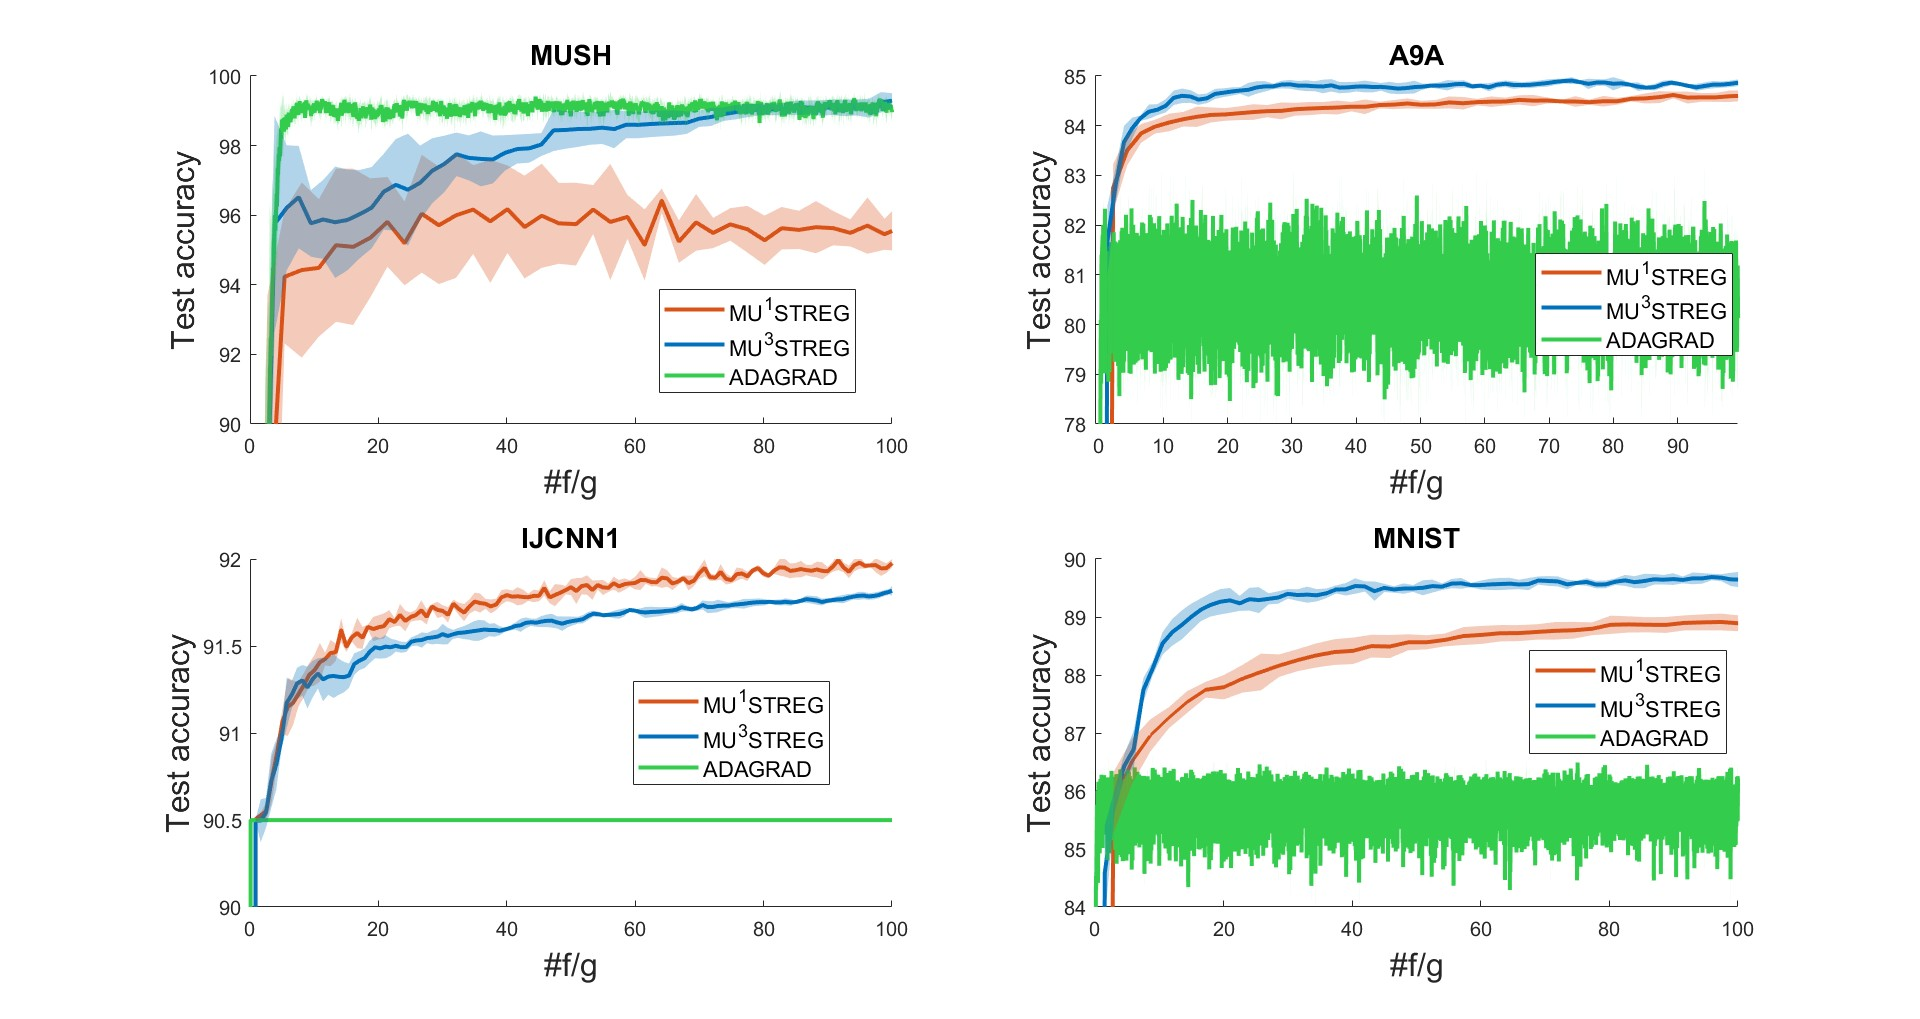
\includegraphics[width=\linewidth]{figures/LEAST-SQUARES_acc_vs_ev_SHADED.jpg}
    \caption{ Classification accuracy on the testing set along the number of  weighted evaluations of gradients and functions.}
    \label{fig: acc vs. ev.}
\end{figure}
	
	\end{frame}
	

			
\end{document}